\input{header}

\begin{document}
\begin{figure}
	\centering
		
\includegraphics[width=1.00\textwidth]{pics/Logo_Deckblatt.pdf}
	\label{fig:logo}
\end{figure}

\setcounter{tocdepth}{3}

\begin{titlepage}

	\begin{center}
	\textcolor{white}{.}
		\vspace{70pt}
		
		\Large{\bfseries{\sffamily{Simulation von infrastrukturellen Umfelderfassungsl�sungen zur Systemkonzeptbewertung}}}
		
		\vspace{15pt}

		\sffamily{Masterarbeit}\\
		\vspace{10pt}
		\normalsize{\sffamily{erstellt von cand. mach. Viviane Bremer}}\\
		\normalsize{\sffamily{Braunschweig, der \today}}
		
		\vspace{18pt}
		\end{center}
	
	\vspace{100pt}
	{\sffamily{Technische Universit�t Braunschweig}}\\
  	{\sffamily{Institut f�r Fahrzeugtechnik}}\\
	{\sffamily{Direktor: Prof. Dr.-Ing. Ferit K���kay}}\\
	{\sffamily{Betreuer: Adrian Sonka}}\\
\end{titlepage}

\newpage
\thispagestyle{empty}~
\thispagestyle{empty}~ 


Aufgabenstellung (Original bzw. Kopie)

\newpage
\renewcommand{\thepage}{\Roman{page}}
\section*{Sperrklausel}
Die Ausgabe der vorliegenden Masterarbeit mit dem Titel "`Simulation von infrastrukturellen Umfelderfassungsl�sungen zur Systemkonzeptbewertung"' ist ausschlie�lich unter Genehmigung der Institutsleitung zul�ssig.

Braunschweig, den \today

\section*{Eidesstattliche Erkl�rung}
Ich versichere an Eides statt, dass ich die vorliegende Bachelor/Master/Studien/Projektarbeit mit dem Titel, ohne unerlaubte fremde Hilfe oder Beratung und nur unter Verwendung der angegebenen wissenschaftlichen Hilfsmittel angefertigt habe.\\
\vspace{10pt}
\begin{table}[htbp]
		\begin{tabular}{l c}
		Ort bei Unterschrift, den Datum bei Unterschrift & \hrulefill \\
		& \textcolor{white}{...............}Name des Autors \textcolor{white}{...............}	\\
		\end{tabular}
\end{table}


\section*{Kurzfassung}
%Inhalt der Kurzfassung

\tableofcontents

\listoffigures
\listoftables
\setcounter{secnumdepth}{-1}
\section{Abk�rzungsverzeichnis}
\setcounter{secnumdepth}{3}

\begin{acronym}[GUIDE]
	\acro{ACC}{Adaptive Cruise Control}
	\acro{ADAC}{Allgemeiner Deutscher Automobil-Club e.V.}
	\acrodefplural{ADAC}[ADAC]{Allgemeine Deutsche Automobil-Club e.V.}
	\acro{CMS}{Collision Mitigation Sys\-tem}
	\acrodefplural{CMS}[CMS]{Collision Mitigation Sys\-teme}
	\acro{IfF}{Institut f�r Fahrzeugtechnik}
\end{acronym}
\setcounter{secnumdepth}{-1}
\section{Symbolverzeichnis}
\setcounter{secnumdepth}{3}
\begin{tabbing}
\hspace{3cm}\=\hspace{2cm}\=\kill
	  %$\mathrm{\Delta h_{ax}}$ \> [m/$\mathrm{s^{2}}$] \> �berschwingweite \\
		$a, c$ \> - \> empirische Koeffizienten\\
		$B$ \> [\unit{m}] \> Breite\\
		$b$ \> [\unit{mm}] \> Basisbreite\\
		$c_L$ \> [\unitfrac{m}{s} \> Lichtgeschwindigkeit\\
		$c_S$ \> [\unitfrac{m}{s}] \> Schallgeschwindigkeit\\
		$D$ \> [\unit{m}] \> Abstand \\
		$d$ \> - \> Disparit�t\\
		$f$ \> [\unit{mm}] \> Brennweite\\
		$f_{Chirp}$ \> [\unitfrac{1}{s}] \> Chirpfrequenz\\
		$f_{Doppler}$ \> [\unitfrac{1}{s}] \> Dopplerfrequenz\\
		$f_0$ \> [\unitfrac{1}{s}] \> Tr�gerfrequenz\\
		$G$ \> - \> Beobachtungsmatrix\\
		$H$ \> [\unit{m}] \> H�he\\
		$I_S$ \> [\unit{W}] \> Schallintensit�t\\
		$k$ \> - \> Zeitschritt\\
		$L$ \> [\unit{m}] \> L�nge\\
		$m_{\omega}$ \> -	\> Treppensteigung der Momentanfrequenz\\
		$P_V$ \> - \> Kovarianz des Beobachtungsrauschens\\
		$P_k$ \> - \> Kovarianzmatrix\\
		$p$ \> - \> Wahrscheinlichkeitsdichte\\
		$p_{Abstand}$ \> [\unit{\%}] \> Erkennungswahrscheinlichkeit des Objektabstandes\\
		$p_{Algorithmus}$ \> [\unit{\%}] \> Erkennungswahrscheinlichkeit des Algorithmus\\
		$p_{Gesamt}$ \> [\unit{\%}] \> Gesamterkennungswahrscheinlichkeit\\
		$p_{Regen}$ \> [\unit{\%}] \> Erkennungswahrscheinlichkeit bei Regen\\
		$p_{Tag}$ \> [\unit{\%}] \> Erkennungswahrscheinlichkeit der Tageszeit\\
		$p_{Witterung}$ \> [\unit{\%}] \> Erkennungswahrscheinlichkeit der Witterung\\
		$R$ \> [\unitfrac{mm}{h}] \> Regenrate\\
		$R_{max}$ \> [\unit{m}] \> maximale Reichweite\\
		$R_{min}$ \> [\unit{m}] \> minimale Reichweite\\
		$S$ \> - \> stochastisches Systemrauschen\\
		$s$ \> [\unit{m}] \> Senderabstand\\
		$s_k$ \> - \> Realisierung des stochastischen Systemrauschens\\
		$s_p$ \> [\unit{$\mu$m}] \> Gr��e des Bildpunktes\\
		$T_{Mess}$ \> [\unit{ms}] \> Messlatenz\\
		$V$ \> - \> stochastisches Beobachtungsrauschen\\
		$v_k$ \> - \> Realisierung des stochastischen Beobachtungsrauschen\\
		$W^{i}_{k}$ \> - \> Gewicht\\
		$X_k$ \> - \> zu sch�tzende Gr��en\\
		$X_l$ \> - \> Bildpunkt links\\
		$X_r$ \> - \> Bildpunkt rechts\\
		$X_W$ \> - \> Weltpunkt\\
		$x, y, z$ \> - \> Raumkoordinaten\\
		$x_0, y_0, z_0$ \> - \> Koordinatenursprung\\
		$Y_k$ \> - \> Beobachtungen\\
		$z_C$ \> [\unit{m}] \> Abstand zwischen Bildebene und Weltpunkt\\
		$\alpha$ \> [\unit{�}] \> horizontaler Ausrichtungswinkel\\
		$\beta$ \> [\unit{�}] \> vertikaler Ausrichtungswinkel\\
		$\Delta T_{Delay_{Min}}$ \> [\unit{ms}] \> Zeitversatz zwischen Realit�t und Modell\\
		$\Delta t$ \> [\unit{s}] \> Laufzeit\\
		$\Delta \phi$ \> [\unit{�}] \> Winkelaufl�sung\\
		$\rho_L$ \> [\unit{\%}] \> Reflexionsgrad des Lichts\\
		$\rho_S$ \> [\unit{\%}]	\> Reflexionsgrad des Schalls\\
		$\pi$ \> - \> Kreiszahl\\
		$\phi$ \> [\unit{�}] \> �ffnungswinkel\\
		$\phi_h$ \> [\unit{�}] \> horizontaler �ffnungswinkel\\		
		$\phi_v$ \> [\unit{�}] \> vertikaler �ffnungswinkel\\
		$\omega_{obj}$ \> [\unitfrac{1}{s}] \> Objektkreisfrequenz\\
		$\omega_0$ \> [\unitfrac{1}{s}] \> Eigenkreisfrequenz\\
\end{tabbing}
%\begin{tabularx}{{\textwidth}{p{2cm}p{2cm}X}
		%$D$ & [\unit{m}] & Abstand \\
		%$c_S$ & [\unitfrac{m}{s}] & Schallgeschwindigkeit\\
		%$\Delta t$ & [\unit{s}] & Laufzeit\\
		%$d$ & [\unit{m}] & Senderabstand\\
		%$I_S$ & [\unit{W}] & Schallintensit�t\\
		%$\rho_S$ & -	& Reflexionsgrad des Schalls\\
		%$m_{\omega}$ & -	& Treppensteigung der Momentanfrequenz\\
		%$c_L$ & [\unitfrac{m}{s} & Lichtgeschwindigkeit\\
		%$r$ & [\unit{m} & Abstand\\
		%$f_{Doppler}$ & [\unitfrac{1}{s}] & Dopplerfrequenz\\
		%$f_{Chirp}$ & [\unitfrac{1}{s}] & Chirpfrequenz\\
		%$f_0$ & [\unitfrac{1}{s}] & Tr�gerfrequenz\\
		%$\rho_L$ & - & Reflexionsgrad des Lichts\\
		%$X_W$ & - & Weltpunkt\\
		%$X_l$ & - & Bildpunkt links\\
		%$X_r$ & - & Bildpunkt rechts\\
		%$b$ & [\unit{m}] & Basisbreite\\
		%$d$ & - & Disparit�t\\
		%$s_p$ & [\unit{m}] & Gr��e des Bildpunktes\\
		%$z_C$ & [\unit{m}] & Abstand\\
		%$Y_k$ & - & Beobachtungen\\
		%$X_k$ & - & zu sch�tzende Gr��en\\
		%$k$ & - & Zeitschritte\\
		%$S$ & - & stochastisches Systemrauschen\\
		%$s_k$ & - & Realisierung des stochastischen Systemrauschens\\
		%$V$ & - & stochastisches Beobachtungsrauschen\\
		%$v_k$ & - & Realisierung des stochastischen Beobachtungsrauschen\\
		%$p$ & - & Wahrscheinlichkeitsdichte\\
		%$P_k$ & - & Kovarianzmatrix\\
		%$G$ & - & Beobachtungsmatrix\\
		%$P_V$ & - & Kovarianz des Beobachtungsrauschens\\
		%$W^{i}_{k}$ & - & Gewicht\\
		%$\Delta T_{Delay_{Min}}$ & [\unit{ms}] & Zeitversatz zwischen Realit�t und Modell\\
		%$T_{Mess}$ & [\unit{ms}] & Messlatenz\\
		%$\Phi$ & [\unit{�}] & �ffnungswinkel\\
		%$\Phi_v$ & [\unit{�}] & vertikaler �ffnungswinkel\\
		%$\Phi_h$ & [\unit{�}] & horizontaler �ffnungswinkel\\
		%$R_{max}$ & [\unit{m}] & maximale Reichweite\\
		%$R_{min}$ & [\unit{m}] & minimale Reichweite\\
		%$x, y, z$ & - & Raumkoordinaten\\
		%$x_0, y_0, z_0$ & - & Koordinatenursprung\\
		%$L$ & [\unit{m}] & L�nge\\
		%$B$ & [\unit{m}] & Breite\\
		%$H$ & [\unit{m}] & H�he\\
		%$\pi$ & - & Kreiszahl\\
		%$\alpha$ & [\unit{�}] & horizontaler Ausrichtungswinkel\\
		%$\beta$ & [\unit{�}] & vertikaler Ausrichtungswinkel\\
		%$\Delta \Phi$ & [\unit{�}] & Winkelaufl�sung\\
		%$p_{Gesamt}$ & - & Gesamterkennungswahrscheinlichkeit\\
		%$p_{Algorithmus}$ & - & Erkennungswahrscheinlichkeit des Algorithmus\\
		%$p_{Witterung}$ & - & Erkennungswahrscheinlichkeit der Witterung\\
		%$p_{Regen}$ & - & Erkennungswahrscheinlichkeit bei Regen\\
		%$p_{Tag}$ & - & Erkennungswahrscheinlichkeit der Tageszeit\\
		%$p_{Abstand}$ & - & Erkennungswahrscheinlichkeit des Objektabstandes\\
		%$R$ & [\unitfrac{mm}{h}] & Regenrate\\
		%$a, c$ & - & empirische Koeffizienten\\
%\end{tabularx}


\renewcommand{\thepage}{\arabic{page}}
\setcounter{page}{1}
\section{Einleitung}
\label{chap:Einleitung}
Seit �ber 10 Jahren besteht ein gro�es Aktivit�tsfeld im Bereich des vernetzten und automatisierten Fahrens. Das Ziel ist die Automatisierung des Verkehrs, um die Mobilit�t energieeffizient, komfortabel, sicher und verkehrseffizient zu gestalten \cite{Bengler.2018}.

Um dies zu erreichen, werden verschiedene Konzepte erarbeitet, bei denen Fahrzeuge und Infrastruktur mit Sensorik zur Umfelderfassung ausgestattet werden, wie z.B. in \cite{Vivacqua.2017} und \cite{Dotzauer2017}. Diese Konzepte sollen f�r die drahtlose Informationsweitergabe des so erfassten fahrzeugspezifischen Lagebildes zwischen den Verkehrsteilnehmern genutzt werden \cite{Bengler.2018}. Dadurch entstehen generelle Fragestellungen bez�glich des Aufbaus und der Architektur der entstehenden L�sungen. Um diese Systemkonzepte noch vor ihrem Einsatz zu analysieren, wird ein Auslegungstool ben�tigt.

Ziel dieser Arbeit ist die Erstellung eines Simulations-Tools, um Systemkonzepte zielgerichtet auszulegen, zu analysieren und zu bewerten. Hierf�r m�ssen die einzelnen Sensoreigenschaften herausgearbeitet und systematisch abgebildet werden.

Kapitel\,\ref{chap:Grundlagen} erl�utert zun�chst die Funktionsweisen und Eigenschaften der Umfelderfassungssensoren Ultraschall, Radar, Lidar und Kamera. Anschlie�end wird auf die Datenverarbeitung eingegangen. Hierzu geh�rt die Objekterkennung, das Tracking und die Sensordatenfusion. In Kapitel\,\ref{chap:Einsatz} werden bestehende Systemkonzepte bei Fahrzeugen und in der Infrastruktur vorgestellt. Anschlie�end werden in Kapitel\,\ref{chap:Anforderungen} die Anforderungen an ein Simulations-Tool zur Systemkonzeptbewertung herausgearbeitet. Die Umsetzung des Tools wird in Kapitel\,\ref{chap:Software-Tool} vorgestellt. Kapitel\,\ref{chap:Anwendung} umfasst die Anwendung des Tools f�r verschiedene Systemkonzepte. In Kapitel\,\ref{chap:Zusammenfassung} werden m�gliche Erweiterungen des Tools, die im Rahmen dieser Arbeit nicht implementiert worden sind, vorgestellt.

 %mit Hilfe von Daten der Forschungskreuzung in Braunschweig.

\section{Umfelderfassung}
\label{sec:TechnikStand}
Dieses Kapitel stellt zun�chst Sensoren zur Umfelderfassung vor und erl�utert deren Funktionsprinzipien. Anschlie�end wird auf die Sensordatenverarbeitung eingangen. Dazu geh�ren die Datenfusion, die Objekterkennung und das Tracking. Auf diesen Grundlagen aufbauend werden in den Abschnitten \ref{sec:KFZSensor} und \ref{sec:InfraSensor} Anwendungen im Fahrzeug und in der Infrastruktur erl�utert.

\subsection{Sensoren zur Umfelderfassung}
\label{sec:Sensoren}
Die Sensoren zur Umfelderfassung werden in entfernungsgebende und bildgebende Sensoren unterschieden. Zu ersterem geh�ren der Ultraschall, das Radar und ddas Lidar. Zu letzterem die Kamera mit dem sichtbaren und dem Infrarotspektrum. Im Folgenden werden die einzelnen Sensorprinzipien erl�utert.

\subsubsection{Ultraschall}
\label{sec:Ultraschall}

Als Ultraschall werden die Schallfrequenzen ab \unit{20}{kHz} bezeichnet. Sie sind f�r das menschliche Ohr nicht h�rbar. Die Messung mit Ultraschall geh�rt zu den Laufzeitmessungen. Ein Sender emittiert Schallwellen, die von Objekten reflektiert werden. Zur Schallerzeugung und -empfang wird bei Ultraschallsensoren eine Membran aus einer Piezokeramik eingesetzt \cite{Winner.2015}. Zum Aussenden der Schallwellen wird die Membran aktiv in Schwingung versetzt und nach einer festgelegten Sendedauer wieder zur Ruhe gebracht. Die Laufzeit $\Delta t$ bis der reflektierte Schall die Membran wieder zur Schwingung anregt wird gemessen. Diese wird zusammen mit der Schallgeschwindigkeit $c_S$ genutzt um den Abstand $D$ zu bestimmen \cite{Trankler.2014}:
\begin{equation}
D = \dfrac{c_S}{2} \Delta t.
\label{eq:AbstandU}
\end{equation}

Da die Strecke zwischen Sender und Objekt zweimal durchlaufen wird, muss sie halbiert werden um den tats�chlichen Abstand zu erhalten. Neben der reinen Abstandsmessung kann mit Hilfe von zwei Sendern, deren Erfassungsbereiche �berlappen, auch eine Positionsbestimmung durchgef�hrt werden. Hierzu wird das Trilaterationsverfahren genutzt. F�r ein rundes Objekt ist dies in Abbildung \ref{fig:Trilateration} dargestellt. Der Abstand $D$ berechnet mittels der Direktechos DE und des Satzes von Pythagoras:
\begin{equation}
D = \sqrt{\text{DE1}^2 - \dfrac{\left(d^2 + \text{DE1}^2-\text{DE2}^2\right)^2}{4d^2}}
\label{eq:PosD}
\end{equation}

\begin{figure}%
\centering
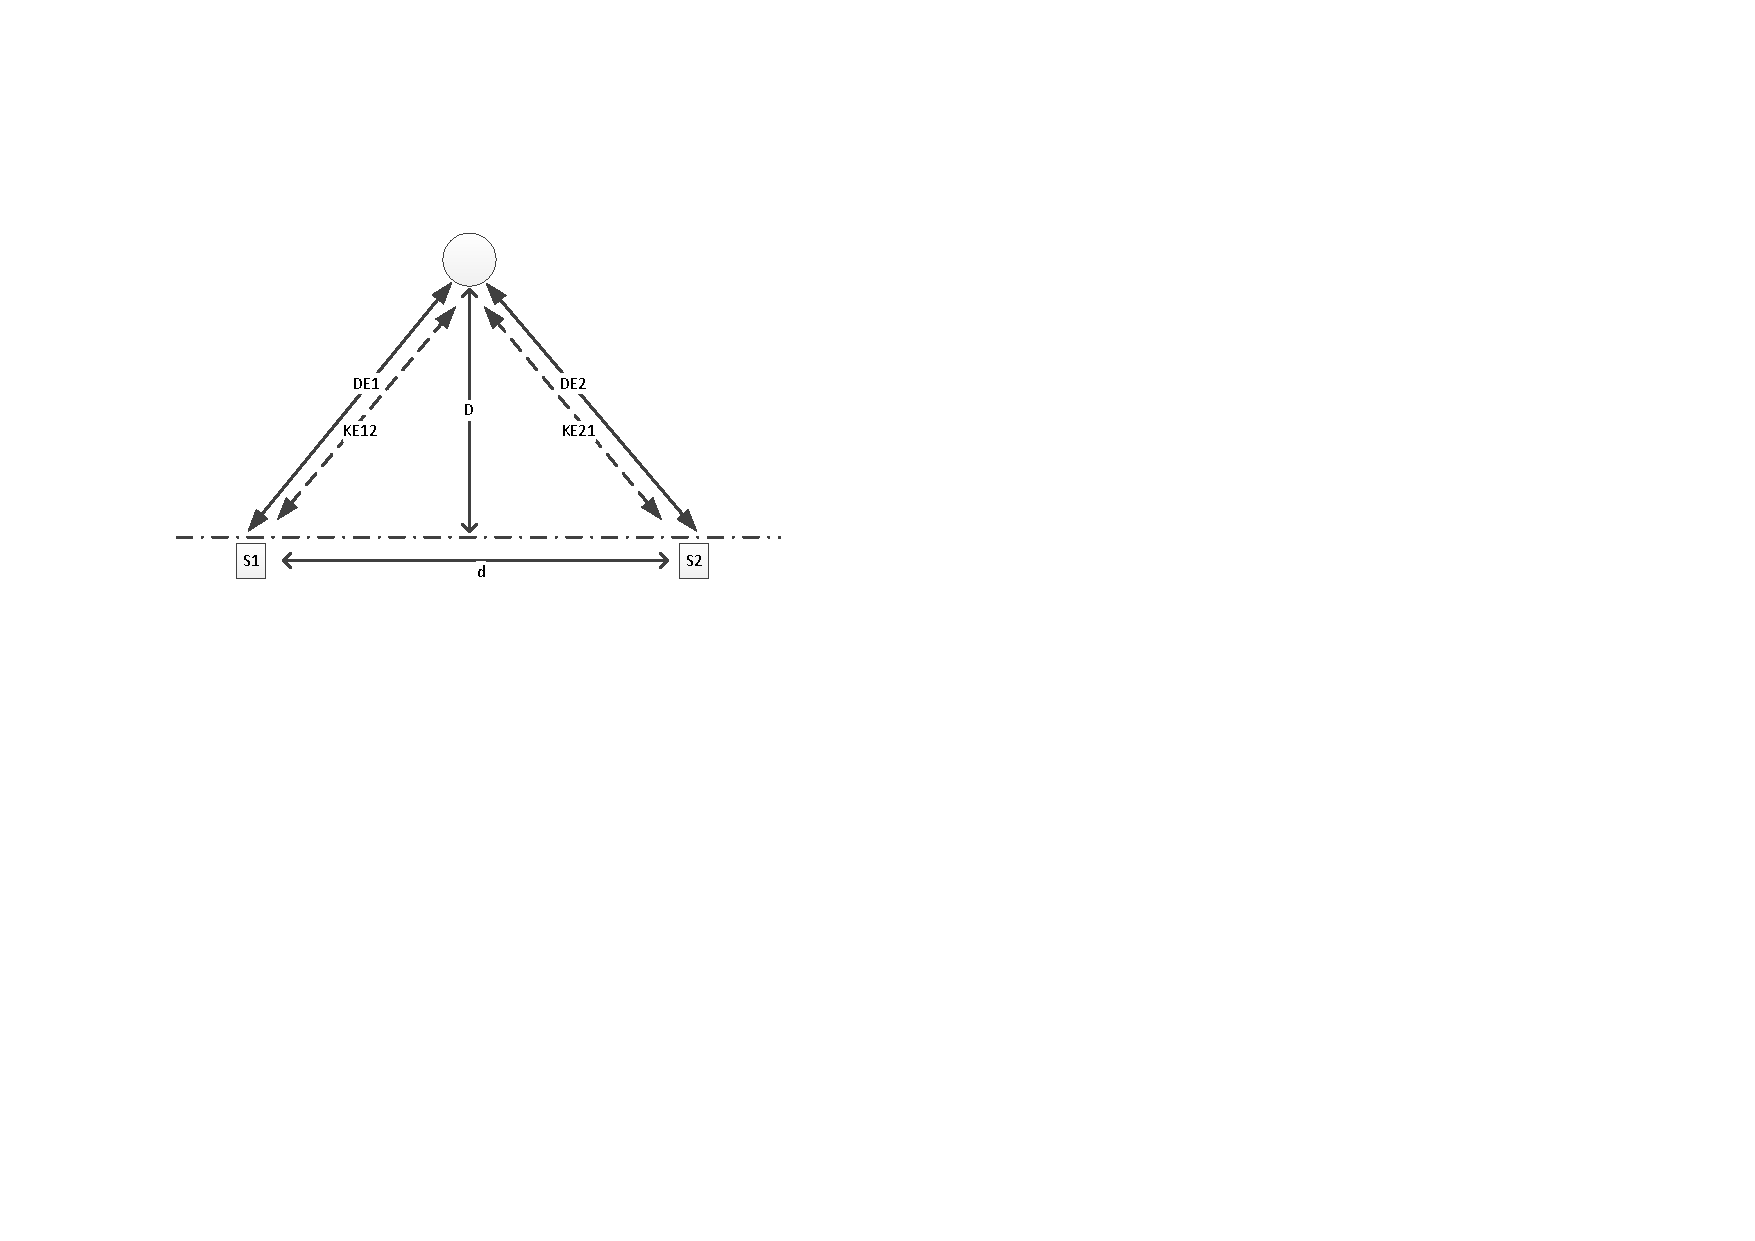
\includegraphics[width=0.6\textwidth,trim={2cm 11cm 16cm 3.5cm},clip]{pics/Position_Ultraschall.pdf}%
\caption{Veranschaulichung des Trilaterationsprinzips f�r ein rundes Objekt}%
\label{fig:Trilateration}%
\end{figure}

Mit Hilfe des Kreuzechos KE kann des Weiteren bestimmt werden, ob es sich um ein rundes Objekt handelt oder um eine Wand. F�r ein rundes Objekt ergibt sich das Kreuzecho KE zu
\begin{equation}
\text{KE}_{rund} = \dfrac{\text{DE1} + \text{DE2}}{2}
\label{eq:KE_rund}
\end{equation}

und f�r eine Wand zu
\begin{equation}
\text{KE}_{Wand} = \sqrt{\dfrac{d^2}{4} + \text{DE1} \times \text{DE2}}.
\label{eq:KE_Wand}
\end{equation}

Die Reichweite des Ultraschallsensors ist abh�ngig von der ausgesendeten Schallintensit�t $I_S$, die in Abh�ngigkeit von der Entfernung $D$ des gemessenen Objektes abnimmt. Somit ergibt sich mit der effektiven Reflexionsfl�che $\sigma$ und bezogen auf den Normabstand $D_1$ die reflektierte Schallintensit�t 
\begin{equation}
I_{refl}=\sigma I_s \left(\dfrac{D_1}{2D}\right)^2.
\label{eq:Irefl}
\end{equation}

Des Weiteren verringern der Reflexionsgrad $\rho_S$ und die Impedanz der Atmosph�re die Schallintensit�t bei der Reflexion. Als untere Grenze zur Objektmessung muss die Schallintensit�t des Empfangssignals oberhalb des Messrauschens liegen, d.h. \unit{$\geq$10}{dB} sein.

\subsubsection{Radar}
\label{sec:Radar}

Die Radarmessung (Radio Detection And Ranging) geh�rt zu den ber�hrungslosen Messverfahren und wird insbesondere bei anspruchsvollen Umgebungsbedingungen eingesetzt \cite{Trankler.2014}. Bei diesem Verfahren werden elektromagnetische Wellen im Mikrowellenbereich eingesetzt, welche kaum anf�llig gegen�ber Temperaturschwankungen und Nebel sind. F�r den Automobilbereich sind die Frequenzen \unit{24}{GHz} und \unit{77}{GHz} reserviert \cite{Winner.2015}. Das \unit{24}{GHz}-Band wird f�r das Short Range Radar (SRR) genutzt und das \unit{77}{GHz}-Band f�r das Long Range Radar (LRR).

Zur Abstands- und Geschwindigkeitsmessung finden zwei verschiedene Ans�tze Verwendung, die sich in der Frequenzmodulation unterscheiden: Das Dauerstrichradar (FMCW -- Frequency Modulated Continous Wave) und die Chirp Frequence Modulation. Die Frequenzverl�ufe der beiden Modulationsverfahren sind in Abbildung \ref{fig:RadarFrequenzverlauf} dargestellt.

\begin{figure}[h]%
\centering
\subfigure[\label{fig:RadarFMCW}]{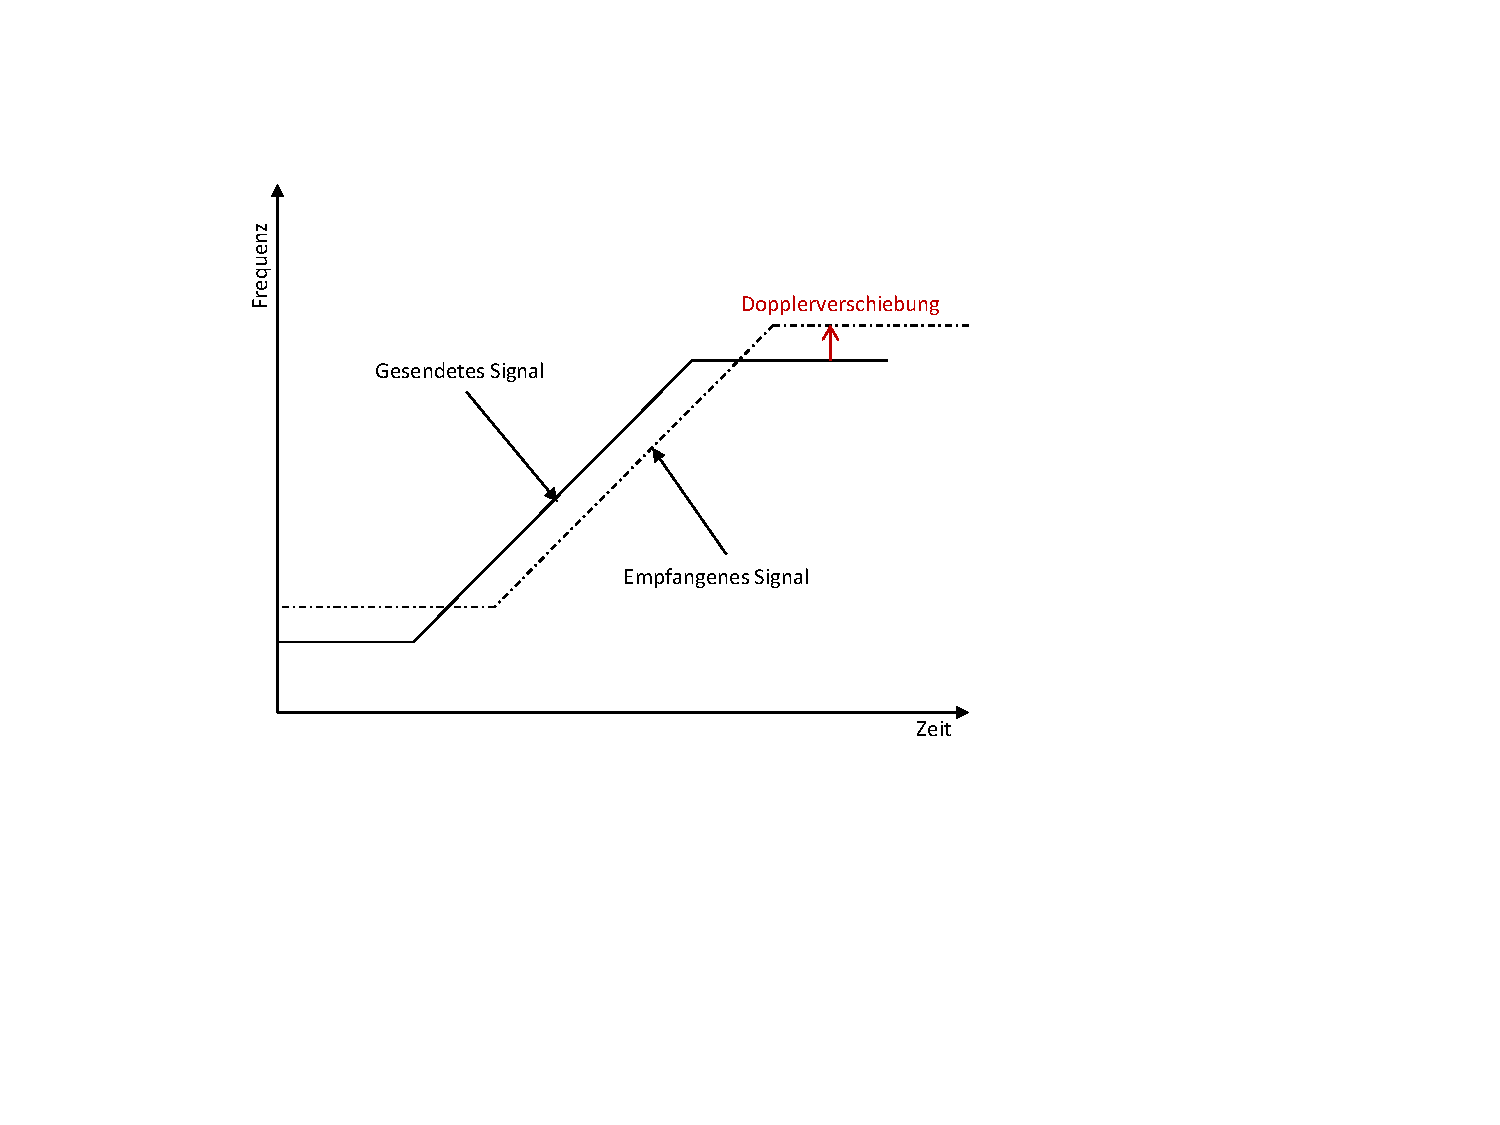
\includegraphics[page=1,width=0.48\textwidth,trim={4cm 6.5cm 8cm 3cm},clip]{pics/Radarsignale.pdf}}
    \subfigure[\label{fig:RadarChirp}]{\includegraphics[page=2,width=0.48\textwidth,trim={4cm 6.5cm 8cm 3cm},clip]{pics/RadarSignale.pdf}}
\caption{Beispielhafter Frequenzverlauf von FMCW (a) und Chirp Frequence Modulation (b) \cite{Winner.2015}}%
\label{fig:RadarFrequenzverlauf}
\end{figure}

Das Dauerstrichradar erzeugt durch die kontinuierliche und rampenf�rmige Ver�nderung der Momentanfrequenz mit der Treppensteigung $m_{\omega}$ eine konstante Phasenverschiebung von $+(2r/c)^2m_{\omega}$. Der Abstand und die Geschwindigkeit wird bei diesem Verfahren mithilfe der Frequenzverschiebung bestimmt:
\begin{align}
	r &= \dfrac{c}{2} \cdot \dfrac{\omega_{obj,1}-\omega_{obj,2}}{m_{\omega,1} - m_{\omega,2}},\\
	\dot{r} &= \dfrac{c}{2 \omega_0} \cdot \dfrac{m_{\omega,1}\omega_{obj,1}-m_{\omega,2}\omega_{obj,2}}{m_{\omega,1} - m_{\omega,2}}.
	\end{align}
	
Mit der Startkreisfrequenz $\omega_0$ und der Kreisfrequenz $\omega_{obj}=\dfrac{2}{c}\left(m_{\omega}r + \omega_0 \dot{r}\right)$.

Bei der Chirp Frequence Modulation wird ein S�gezahnsignal mit einem Hub von $f_{chirp}=30...300\,\text{MHz}$ erzeugt. Die Dopplerfrequenz bestimmt hierbei die Wiederholrate und sollte etwa \unit{80}{kHz} betragen, um Mehrdeutigkeiten zu vermeiden. Der Abstand $r$ wird mit dem Puls-Doppler-Verfahren mit der Laufzeit $t_{of}=t_{PC}-t_S$, bezogen auf die Pulsmitte $t_{PC}$, und der Lichtgeschwindigkeit $c_L$ bestimmt. F�r die Geschwindigkeit $\dot{r}$ wird die Dopplerfrequenz $f_{Doppler}$ und die Tr�gerfrequenz $f_0$ genutzt.
\begin{align}
	r &= \dfrac{1}{2}c_L t_{of}\\
	\dot{r} &= - \dfrac{c_L}{2} \dfrac{f_{Doppler}}{f_0}
\end{align}

Der Doppler-Effekt besagt, dass sich die Frequenz bei der Reflexion in Abh�ngigkeit von der �nderung des Abstandes $\dot{r}$ �ndert. Diese Frequenz wird Dopplerfrequenz $f_{Doppler}$ genannt. Beim Ann�hern ($\dot{r}<0$) ist diese Frequenz positiv und beim Entfernen negativ.

Die Reichweite des Radars ist abh�ngig von der Sendeleistung und der Richtcharakteristik der Antenne. Je nach Richtcharakteristik ergibt sich der Antennengewinn $G$, der Einfluss auf die Reichweite nimmt. So ergibt sich die Empfangsleistung f�r ein reflektiertes Radarsignal zu
\begin{equation}
P_R = \dfrac{10^{-2kr/1000}  \sigma  \lambda^2  G^2  V_{mp}^2  P_{total}}{(4\pi)^3 r^4}
\label{eq:Empfangsleistung}
\end{equation}

mit dem R�ckstreuquerschnitt des Objektes
\begin{equation}
\sigma_{plate} = 4\pi \dfrac{A^2}{\lambda^2}.
\label{eq:Rueckstreuquerschnitt}
\end{equation}

Gleichung \ref{eq:Empfangsleistung} ber�cksichtigt au�erdem sogenannte Signalleistungssch�ttler mit dem Faktor $V_{mp}^2$, $0 \leq V_{mp} \leq 2$.

F�r die Winkelbestimmung kommen zwei verschiedene Verfahren zum Einsatz. Das erste Verfahren ist das mechanische Scanning, bei dem eine Strahlablenkeinheit oder eine Planarantenne mechanisch geschwenkt wird. Dabei rotiert die Radarkeule mit einer Schrittweite von etwa \unit{1}{�}, siehe Abbildung \ref{fig:RadarScan}.

Das zweite Verfahren ist das Monopuls-Verfahren. Hierbei erzeugt eine separate Antenne einen Sendestrahl, der von einer Doppelantennen-Anordnung empfangen wird, siehe Abbildung \ref{fig:RadarMonopuls}. Eine Verbesserung dieses Verfahrens wird durch die Verwendung von Mehrstrahlern mit bis zu vier Antennen erm�glicht.

\begin{figure}[h]%
\centering
\subfigure[\label{fig:RadarScan}]{\includegraphics[page=1,width=0.4\textwidth,trim={6.5cm 5cm 8cm 4cm},clip]{pics/RadarFoV.pdf}}
    \subfigure[\label{fig:RadarMonopuls}]{\includegraphics[page=2,width=0.4\textwidth,trim={6.5cm 5cm 8cm 4cm},clip]{pics/RadarFoV.pdf}}
\caption{Schematische Darstellung des Scanning Verfahrens (a) und des Monopuls Verfahrens (b) \cite{Winner.2015}}%
\end{figure}

\subsubsection{Lidar}
\label{sec:Lidar}

Light Detection and Ranging, kurz Lidar, geh�rt zu den optischen Messverfahren und nutzt UV-, IR-Strahlen oder Strahlen aus dem sichtbaren Spektrum \cite{Winner.2015}. F�r die Abstandsmessung wird die Pulslaufzeitmessung genutzt, bei dem kurze Lichtblitze hoher Leistung, meist Laser-Pulse, gesendet und die Laufzeit gemessen wird \cite{Trankler.2014}. Der Abstand wird analog zum Ultraschall bestimmt:
\begin{equation}
d = \dfrac{c_L \Delta t}{2}
\label{eq:AbstandL}
\end{equation}

Mit der Lichtgeschwindigkeit $c_L$. Die Reichweite beim Lidar ist durch die Lichtintensit�t, welche den Laserschutzvorschriften gen�gen muss, beschr�nkt. Des Weiteren beeinflusst auch der Reflexionsgrad $\rho_L$ die Reichweite. Dieser ist insbesondere von der Oberfl�che des Objektes abh�ngig, aber auch von seiner Gr��e. So ergibt sich f�r die reflektierte Lichtintensit�t $P_{r,gro�}$ f�r ein gro�es bzw. nahes Objekt die folgende Gleichung:
\begin{equation}
P_{r,gro�} = \dfrac{\rho_L \cdot A_t \cdot H \cdot T^2 \cdot P_t}{\pi^2 \cdot R^3 \cdot (Q_v/4)(\Phi/2)^2}
	\label{eq:Pgross}
\end{equation}

F�r ein Objekt, das -- aufgrund der Entfernung -- kleiner ist als der Lichtpunkt, �ndert sich Gleichung \ref{eq:Pgross} zu:
\begin{equation}
P_{r,klein} = \dfrac{\rho_L \cdot A_t \cdot H \cdot T^2 \cdot P_t}{\pi^2 \cdot R^4 \cdot (Q_v Q_h/4)(\Phi/2)^2}. 
\label{eq:Pklein}
\end{equation}

Hierbei ist $\Phi$ der Winkel der Objektreflexion, $H$ die Objektbreite, $A_t$ die Empfangslinsenfl�che, $T$ die Transmission der Atmosph�re, $Q_v$ und $Q_h$ die vertikale bzw. horizontale Strahldivergenz und $P_t$ die Laserleistung.

Das Sichtfeld kann von dem eindimensionalen Fall mit einem Strahl in nur eine Richtung auch horizontal und vertikal beliebig erweitert werden. Daf�r gibt es zwei verschiedene Ans�tze. Ein Ansatz ist der Einsatz eines schwenkbaren Spiegels, der den Laserstrahl umlenkt. Hierdurch ist ein horizontaler �ffnungswinkel von bis zu \unit{360}{�} und ein vertikaler �ffnungswinkel von bis zu \unit{120}{�} m�glich. Der zweite Ansatz nutzt ein Array aus Laserdioden, die mittels Multiplexverfahren angesteuert werden. Der horizontale �ffnungswinkel bei dieser Variante betr�gt bis zu \unit{110}{�}. Der vertikale �ffnungswinkel ist von der Strahlbreite abh�ngig und betr�gt in etwa \unit{2}{�} bis \unit{5}{�}.

\subsubsection{Kamera}
\label{sec:Kamera}
Die Kamera geh�rt zu den bildgebenden Sensoren und besitzt dadurch den Vorteil, �hnliche Informationen wie das menschliche Auge zu produzieren \cite{Winner.2015}. Somit k�nnen Objekte mit einer hohen Genauigkeit identifiziert werden. Die Entfernungsmessung mit einer einzelnen Kamera ist hingegen ungenau, da nur anhand der Aufl�sung gesch�tzt werden kann. Auch der Sichtbereich und die Reichweite sind von der Aufl�sung abh�ngig. Letzteres wird durch den Bereich des scharfen Abbildens begrenzt \cite{Hering.2016}. Die untere Grenze $a_v$ der Reichweite liegt vor und die obere Grenze $a_h$ hinter der Objektebene. Sie ergeben sich mit
\begin{align}
a_v &= \dfrac{a f'^2}{f'^2 - u'k(a+f')}\\
a_h &= \dfrac{a f'^2}{f'^2 + u'k(a+f')}.
\label{eq:a_vh}
\end{align}

Dabei ist $k$ die Blendenzahl, $a$ der Abstand zwischen Objektebene und Eintrittspupille, $f'$ die Brennweite und $u'$ der Durchmesser des Unsch�rfekreises, der sich folgenderma�en bestimmen l�sst:
\begin{equation}
u' = \dfrac{\text{Formatdiagonale}}{1000}
\label{eq:u'}
\end{equation}

Neben dem sichtbaren Spektrum k�nnen einige Kameras auch das Infrarotspektrum abbilden. Dadurch ist der Einsatz in der Nacht bzw. Dunkelheit m�glich. Es gibt zwei verschiedene Ans�tze hierbei, die unterschiedliche Infrarotbereiche nutzen \cite{Winner.2015}. Eine M�glichkeit ist das Nahinfrarot (NIR). Hierbei wird die Szene mit NIR-Strahlung ausgeleuchtet, dessen Reflexion von der Kamera erkannt wird. Die andere M�glichkeit ist der Einsatz von Ferninfrarot (FIR). In diesem Spektrum liegt die W�rmestrahlung von Objekten, die von speziellen W�rmebildkameras erfasst werden kann. Ein aktives Beleuchten der Szene enf�llt somit.

%\subsubsection{Sensorvergleich}
%\label{sec:Sensorvergleich}
%
%
%\begin{table}[hb]%
%\centering
%\begin{tabularx}{\textwidth}{lp{2.5cm}p{2.5cm}p{2cm}p{2cm}}
 %& \textbf{Ultraschall} & \textbf{Radar} & \textbf{Lidar} & \textbf{Kamera}\\ \toprule
%\textbf{hor. �ffnungswinkel} & \unit{120}{�} -- \unit{140}{�}& \unit{12}{�} -- \unit{150}{�} & \unit{10}{�}--\unit{360}{�} & \unit{40}{�}--\unit{180}{�}\\ \midrule
%\textbf{ver. �ffnungswinkel} &\unit{60}{�} -- \unit{70}{�}& \unit{4}{�} -- \unit{36}{�}&\unit{2}{�} -- \unit{70}{�}&\unit{6.7}{�} -- \unit{54}{�}\\ \midrule
%\textbf{min. Reichweite} &\unit{0.15}{m}&\unit{0.5}{m}&\unit{0}{m}&--\\ \midrule
%\textbf{max. Reichweite} &\unit{5.5}{m}&\unit{350}{m}&\unit{300}{m}&\unit{3390}{m}\\ \midrule
%\textbf{Geschwindigkeit} & -- & \unitfrac[--400]{km}{h}\newline \unitfrac[+200]{km}{h} & -- & -- \\\midrule
%\textbf{Aufl�sung} & gering & \unit{0.5}{m} -- \unit{1}{m} \newline \unit{3.3}{�} -- \unit{6.}{�} \newline \unitfrac[0.1]{m}{s} -- \unitfrac[1.4]{m}{s}&\unit{0.1}{m}\newline \unit{0.25}{�}& \unit{320x240}{Pixel}\newline \unit{6576x4384}{Pixel}\\ \midrule
%\textbf{Genauigkeit} & -- &\unit{$\pm$0.25}{m}&\unit{$\pm$0.04}{m}& \unit{5.5x5.5}{$\mu$m}\\ \midrule
%\textbf{Messdauer} & \unit{1}{ms}&\unit{50}{s}& \unit{40}{Hz}& \unit{30}{Hz}\\ \bottomrule
%\end{tabularx}
%\caption{Vergleich der Parameter der Sensortypen}
%\label{tab:Sensorparameter}
%\end{table}

\subsection{Datenverarbeitung}
\label{sec:Datenverarbeitung}

Im folgenden Abschnitt wird auf die Datenverarbeitung genauer eingegangen. Sie unterteilt sich in die Objekterkennung und das Objekttracking, welche durch eine Datenfusion erweitert werden k�nnen. Der Ablauf der Datenverarbeitung ist in Abbildung \ref{fig:Datenverarbeitung} schematisch dargestellt.

\begin{figure}[h]
	\centering
		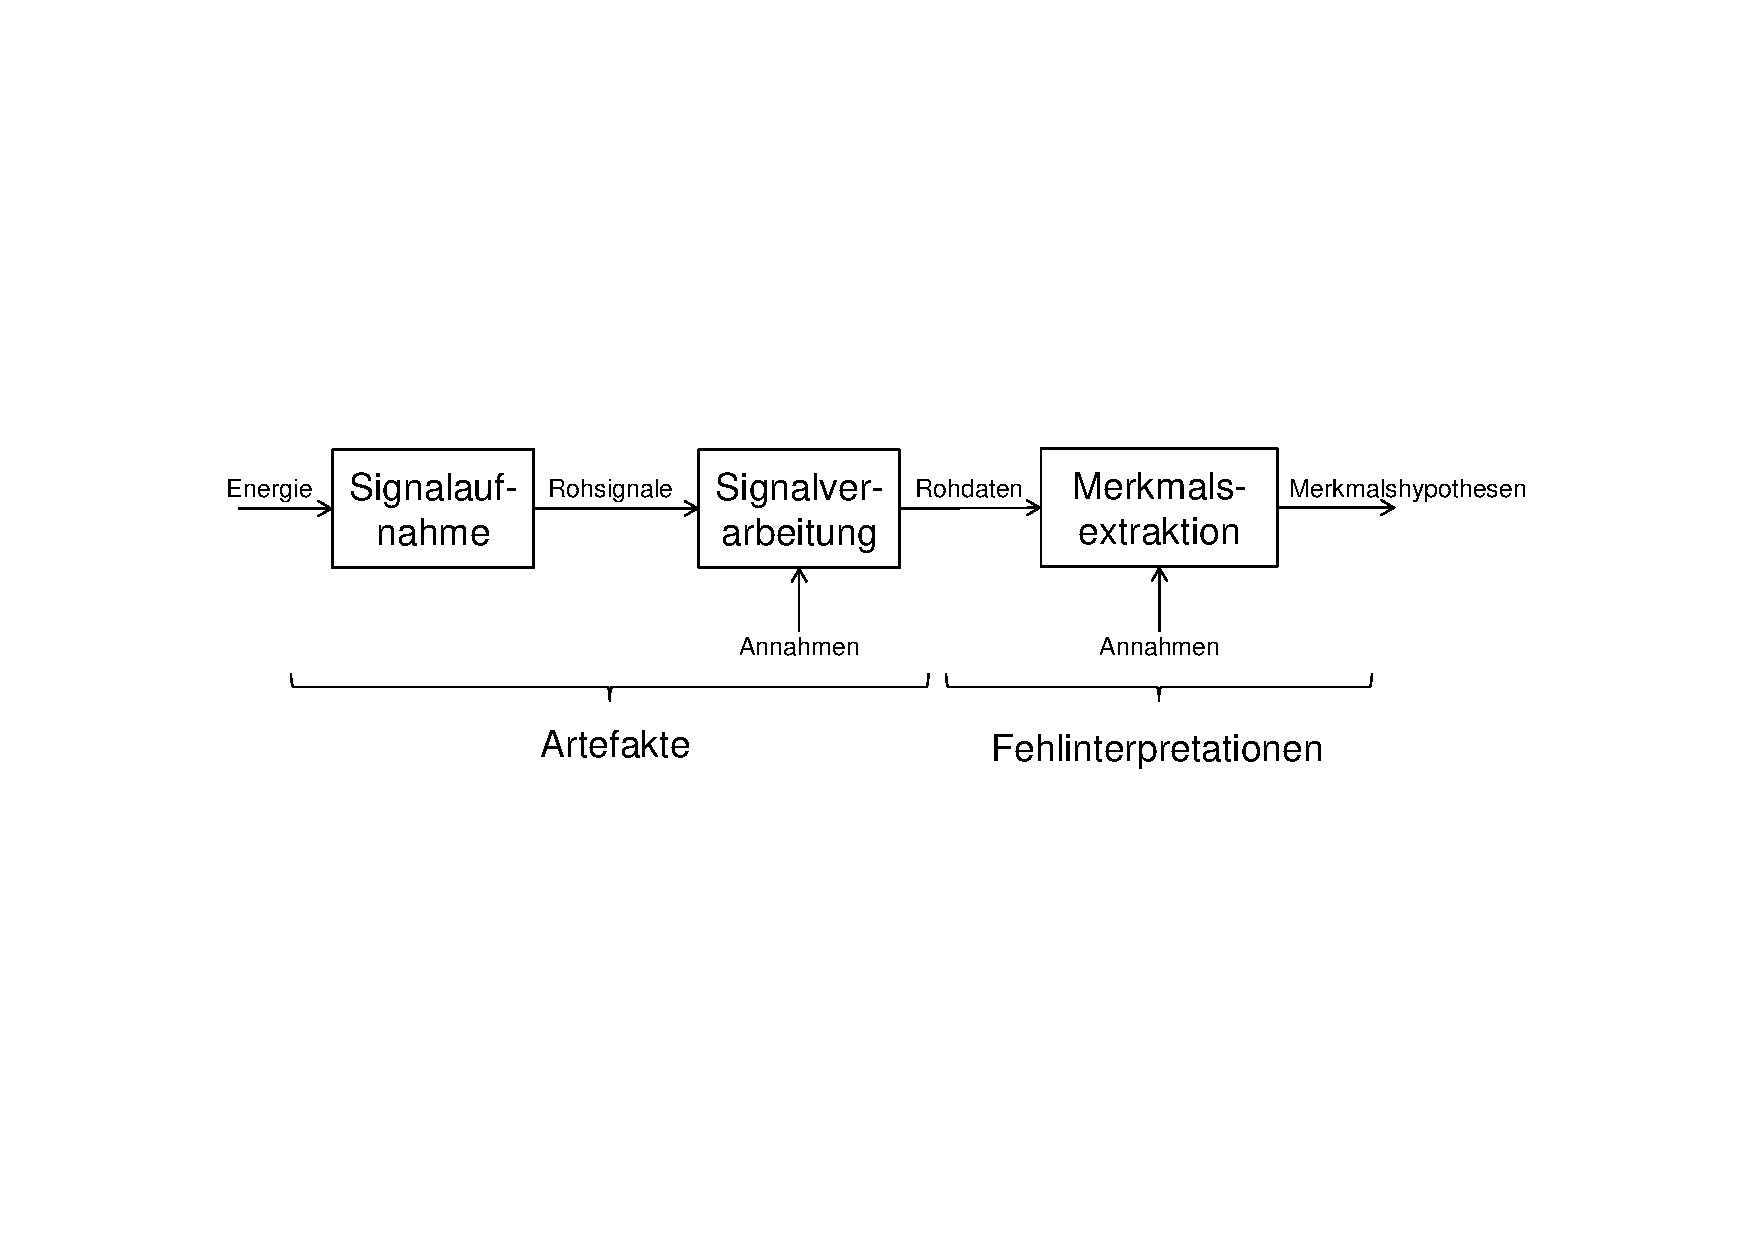
\includegraphics[width=\textwidth,trim={3cm 8cm 3cm 7cm},clip]{pics/Datenverarbeitung.pdf}
	\caption{Schematischer Ablauf der Datenverarbeitung \cite{Winner.2015}}
	\label{fig:Datenverarbeitung}
\end{figure}

Als erstes wird die Signalaufnahme mittels des Sensors durchgef�hrt. Dem schlie�t sich sich eine Signalverarbeitung der Rohsignale an. Danach werden mit Hilfe einer Merkmalsextraktion Merkmals- bzw. Objekthypothesen aufgestellt. Fehlerquellen sind hierbei Artefakte durch Verletzung von physikalischen Annahmen in der Signalverarbeitung und Fehlinterpretationen durch Annahmen in der Merkmalsextraktion.

\subsubsection{Objekterkennung}
\label{sec:Objekterkennung}
Bei der Objekterkennung ist die Wahl des Verfahrens ma�geblich abh�ngig vom Sensortyp. So werden f�r Radar und Lidar z.B. Segmentierungsverfahren eingesetzt und f�r Kamera Gradientenverfahren.

Radar und Lidar erzeugen bei der Messung Punktwolken. Um in diesen Punktwolken Objekte zu identifizieren, werden Segmentierungsverfahren eingesetzt. Die Annahme bei diesem Verfahren ist, dass Messrohpunkte eines Objektes in enger Nachbarschaft liegen. So werden diese Punkte mittels Region-Growing oder Linienextraktion gruppiert bzw. verbunden, siehe Abbildung \ref{fig:RegionGrowingLinie}. Nach diesem Schritt werden die Segmente in I- und L-Formen unterschieden. Unter Verwendung der Segmentabmessungen kann schlie�lich die Objektklasse bestimmt werden \cite{Walchshausl.2008}.

\begin{figure}[h]%
\centering
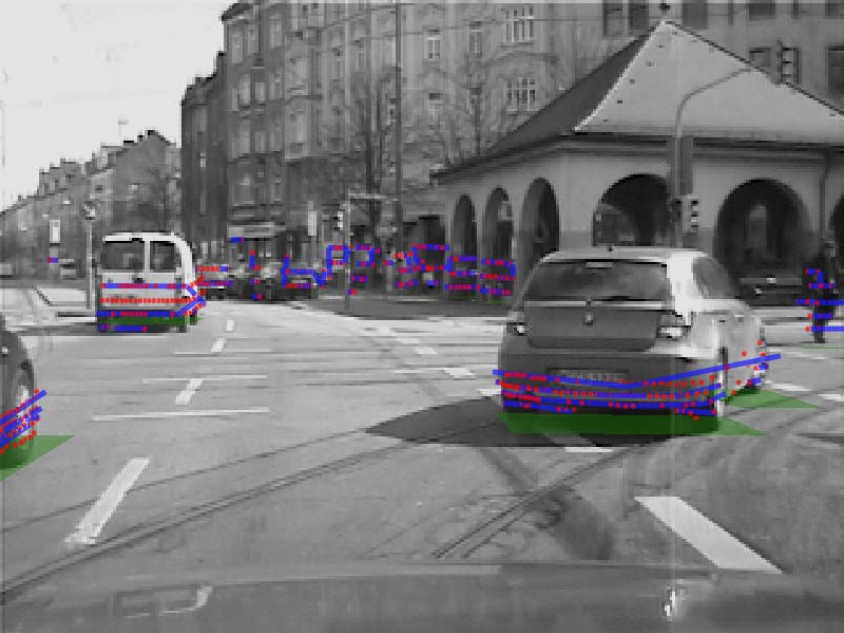
\includegraphics[width=0.6\textwidth]{pics/RegionGrowingVSLinie.PNG}%
\caption{Beispiel f�r den Vergleich von Region-Growing (gr�n) und Linienextraktion (blau). Die roten Punkte sind die Laserscannerrohdaten \cite{Walchshausl.2008}}%
\label{fig:RegionGrowingLinie}%
\end{figure}

Bei der Kamera werden Gradientenverfahren und Matching Verfahren zur Merkmalsextraktion eingesetzt \cite{Winner.2015}. Die wichtigsten Merkmale beim Kamerabild sind Kanten und Ecken. Diese f�hren zu einer deutlichen �nderung des Bildsignals, welche mathematisch durch Gradienten beschrieben wird. Diese k�nnen in Histogramme der Gradientenrichtung �berf�hrt werden, siehe Abbildung \ref{fig:Bildgradienten}. 

\begin{figure}[h]%
\centering
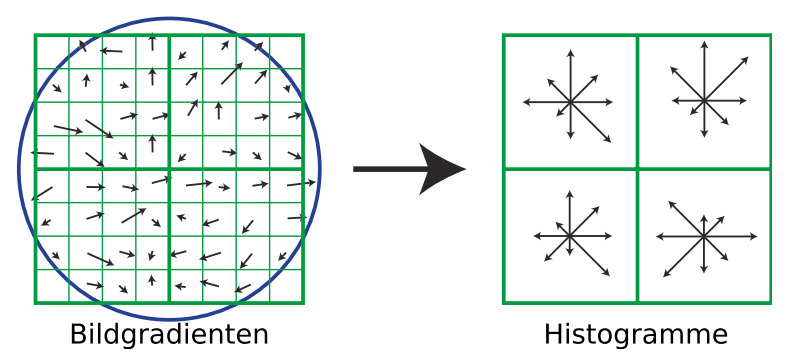
\includegraphics[width=0.6\textwidth]{pics/Gradientenverfahren.PNG}%
\caption{Beispielhafte Darstellung der Bildgradienten (links) und der Histogramme der Gradientenrichtung (rechts) \cite{Winner.2015}}%
\label{fig:Bildgradienten}%
\end{figure}

Beim Matching Verfahren wird eine kleine Region um einen Bildpunkt herum mit den entsprechenden Punkten im n�chsten Bild verglichen. Um nicht den gesamten Bildraum abzusuchen, wird das Verfahren auf Ecken und Kanten im Bild angewendet.

\subsubsection{Tracking}
\label{sec:Tracking}
F�r das Tracking werden insbesondere drei verschiedene Verfahren eingesetzt. Das sind der Bayes-Filter, der Kalman-Filter und der Partikelfilter \cite{Winner.2015}. Die Aufgabe dieser Verfolgungsverfahren ist, aus den Beobachtungen $Y_k$ die zu sch�tzenden Gr��en $X_k$ zu bestimmen. Dies geschieht zu diskreten Zeitschritten $k=1,\, 2,...$. Die Systemgleichung 
\begin{equation}
X_k = f_k\left(X_{k-1},s_k\right)
\label{eq:ZustandXk}
\end{equation}

beschreibt die Dynamik des Zustandes $X_k$. Hierbei wird das stochastische Systemrauschen $S$ mit Hilfe von $s_k$ realisiert. Die erzeugten Beobachtungen $Y_k$ werden mittels der Beobachtungsgleichung
\begin{equation}
Y_k = g_k\left(X_k,v_k\right)
\label{eq:BeobachtungYk}
\end{equation}

beschrieben. $v_k$ ist dabei die Realisierung des stochastischen Beobachtungsrauschens $V$. Mit Hilfe dieser Gleichungen wird die Wahrscheinlichkeitsdichte $p\left(X_k|Y_0...Y_k\right)$ f�r den aktuellen Zustand gesch�tzt.

Der Bayes-Filter ist ein allgemeing�ltiges Verfolgungsverfahren. Es sch�tzt aus der Beobachtung die neue m�gliche Position. Die Beobachtung findet im Zustandsraum statt und gibt eine Wahrscheinlichkeitsdichte f�r den aktuellen Zustand heraus unter Ber�cksichtigung aller vorigen Beobachtungen. Die rekursive Gleichung f�r die Wahrscheinlichkeitsdichte des Bayes-Filters lautet folgenderma�en:
\begin{equation}
p\left(X_k|Y_0,...,Y_{k-1}\right)= c \cdot p\left(Y_k|X_k\right)\cdot \int p\left(X_k|X_{k-1}\right)p\left(X_{k-1}|Y_0,...,Y_{k-1}\right) dX_{k-1}
\label{eq:Bayes}
\end{equation}

Der Kalman-Filter sch�tzt die Zust�nde aufgrund von redundanten Daten. Somit wird zu jedem Zeitpunkt $k$ die Normalverteilung mit Hilfe ihres Mittelwertes $\hat{X_k}$ und der Kovarianzmatrix $P_k$ bestimmt. Die  Sch�tzung aus dem vorigen Schritt $\hat{X}_{k-1}$, $P_{k-1}$ wird f�r die n�chste Position auf den aktuellen Zeitschritt projiziert:
\begin{align}
\hat{X}^{-}_{k}&=F\hat{X}_{k-1}\\
\hat{P}^{-}_{k}&=F\hat{P}_{k-1}F^T+P_S
\end{align}

Dabei ist $F$ die Dynamikmatrix und $P_S$ die Kovarianzmatrix des Systemrauschens. Danach wird schlie�lich die neueste Beobachtung $Y_k$ mit der Beobachtungsmatrix $G$ und der Kovarianzmatrix des Beobachtungsrauschens $P_V$ ber�cksichtigt.
\begin{align}
\hat{X}_{k}&=\hat{X}^{-}_{k} + \hat{P}^{-}_{k}G^T\left(P_V + G\hat{P}^{-}_{k}G^T\right)^{-1} \left(Y_k - GF\hat{X}_{k-1}\right)\\
\hat{P}_{k}&=\hat{P}^{-}_{k}-\hat{P}^{-}_{k}G^T \left(P_V + G\hat{P}^{-}_{k}G^T\right)^{-1}G\hat{P}^{-}_{k}
\end{align}

Beim Partikelfilter wird die Wahscheinlichkeitsdichte durch die endliche Summe von Diracst��en mit Gewichten $w^{i}_{k}p\left(X_k|Y_0,...,Y_k\right)\approx \sum w^{i}_{k}\delta\left(X_k - X^{i}_{k}\right)$ approximiert. Die Paare aus Gewicht $W^{i}_{k}$ und Zustand $X^{i}_{k}$ werden als Partikel betrachtet. Nach jedem Innovationsschritt werden schlie�lich die Gewichte aktualisiert.

\subsubsection{Sensordatenfusion}
\label{sec:Fusion}

Die Sensordatenfusion wird genutzt, um die Genauigkeit zu erh�hen bzw. mehr Informationen zu erhalten. Dies ist davon abh�ngig, welche Sensoren und wie sie eingesetzt werden. Im Allgemeinen werden die Ans�tze in komplement�r, konkurrierend und kooperativ unterschieden. Die Bedeutung f�r den Sensoreinbau ist in Abbildung \ref{fig:Fusionsansaetze} dargestellt. Werden Sensoren komplement�r genutzt, so erg�nzen sich deren einzelne Sichtfelder zu einem gro�en. Sind Sensoren konkurrierend verbaut, sind sie entweder redundant, d.h. es wird die gleiche Information generiert, oder kontr�r, d.h. es werden gegens�tzliche Informationen erzeugt. Der letzte Ansatz ist der kooperative Einsatz von unterschiedlichen Sensoren, die zusammen einen h�heren Informationsgehalt erzeugen \cite{Dietmayer2005}.

\begin{figure}[h]
	\centering
		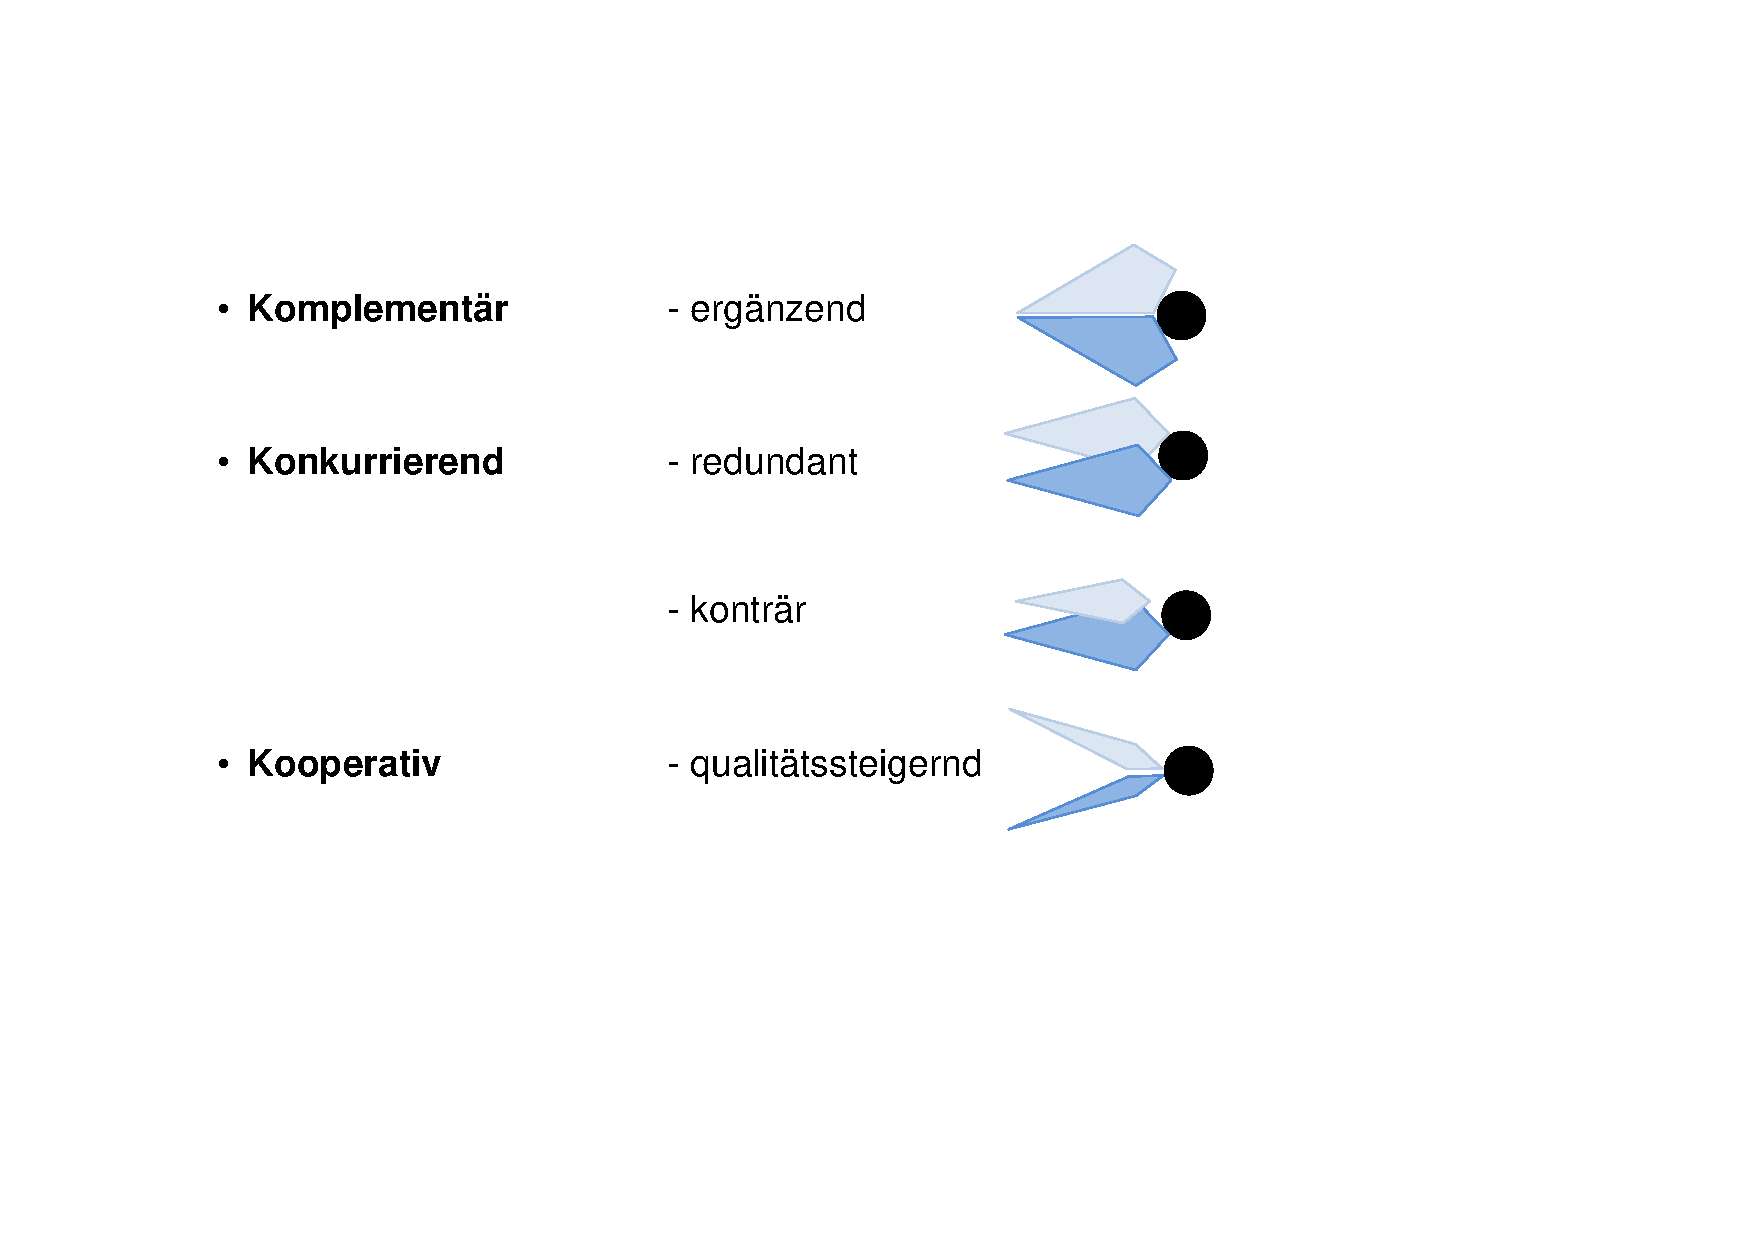
\includegraphics[width=0.6\textwidth,trim={3cm 6.5cm 9cm 4cm},clip]{pics/Fusionsansaetze.pdf}
	\caption{Ans�tze der Datenaufnahme f�r die Datenfusion}
	\label{fig:Fusionsansaetze}
\end{figure}

F�r die Sensordatenfusion gibt es zwei wesentliche Ans�tze, siehe Abbildungen \ref{fig:ImpliziteFusion} und \ref{fig:ExpliziteFusion}. Entweder werden die Daten implizit oder explizit fusioniert. Bei der impliziten Fusion werden die Sensordaten zeitlich nacheinander eingebracht. Dadurch wird eine zeitlich konsistente Datenverarbeitung n�tig. Au�erdem muss eine zeitliche Filterung durchgef�hrt werden, wenn die Messdaten vorliegen. Es wird jedoch schon eine Assoziation auf dem sensorspezifischen Abstraktionslevel durchgef�hrt, die bei der Fusion abgeglichen wird. Vorteilhaft bei der impliziten Fusion ist, dass keine Synchronisierung der Sensoren durchgef�hrt werden muss.

Werden asynchrone Sensoren bei der Datenfusion verwendet, m�ssen die Daten sequentiell eingebracht werden. Somit ist der Algorithmus nicht deterministisch. Zudem k�nnen Quantisierungsfehler auftreten. Insbesondere wenn die Daten des Sensors mit der kleinsten Latenz kurz nach denen vom Sensor mit der gr��ten Latenz eingebracht werden. Dann k�nnen diese Informationen nicht mehr in die Assoziation mitber�cksichtigt werden. Je �hnlicher die Latenzzeiten der einzelnen Sensoren sind, desto geringer wird schlie�lich auch der Fehler der Sch�tzung. 

\begin{figure}[h]
	\centering
		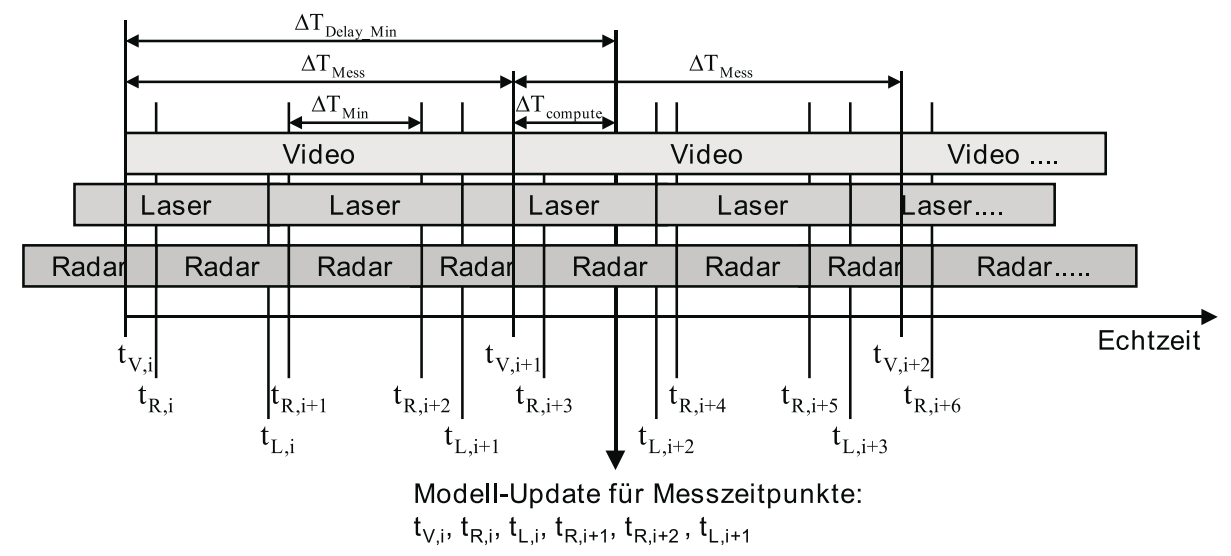
\includegraphics[width=0.9\textwidth]{pics/ImpliziteFusion.PNG}
	\caption{Implizite Sensordatenfusion mit asynchronen Sensoren \cite{Dietmayer2005}}
	\label{fig:ImpliziteFusion}
\end{figure}

Bei der expliziten Fusion wird abgewartet, bis alle Messdaten vorliegen und dann erst fusioniert. Somit findet eine zeitliche Filterung in einem festen Zeitraster statt und die Assoziation findet auf einem gemeinsamen Abstraktionslevel statt. Hierbei m�ssen die Messdaten jedoch synchronisierbar sein.

Die Datenfusion mit synchronen Sensoren f�hrt zu einer sicheren und zuverl�ssigen Assoziation. Da jedoch der Sensor mit der l�ngsten Akquisitionszeit den zeitlichen Versatz zwischen Messung und Assoziation bestimmt, ist der Algorithmus streng deterministisch und es kommt zu einem hohen Verzug zwischen Realwelt und Modell $\Delta T_{Delay_Min}$. Die Arbeit mit synchronisierten Sensoren bietet jedoch neben der sicheren Assoziation eine einfache Erweiterbarkeit um weitere Sensoren.

\begin{figure}[h]
	\centering
		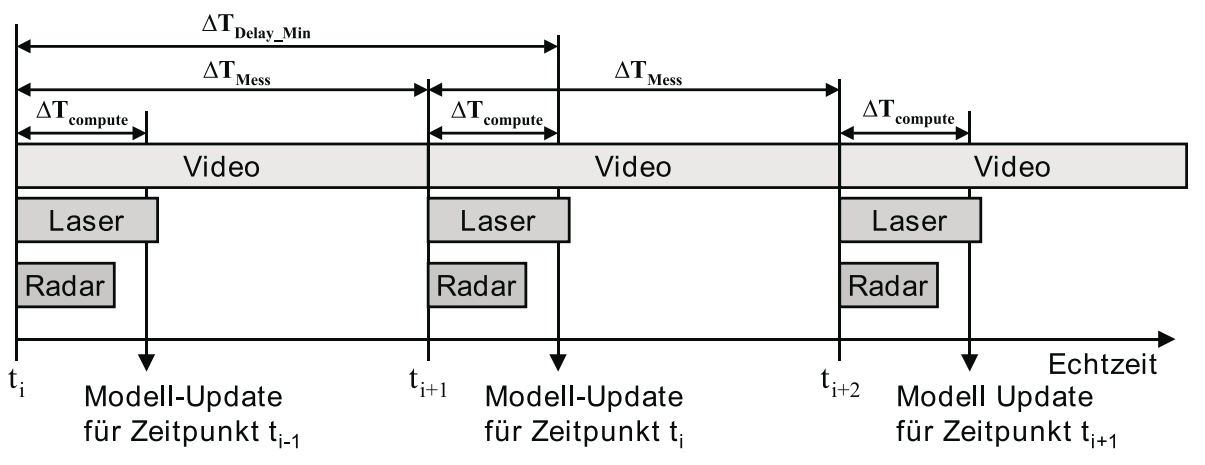
\includegraphics[width=0.9\textwidth]{pics/ExpliziteFusion.PNG}
	\caption{Explizite Sensordatenfusion mit synchronen Sensoren \cite{Dietmayer2005}}
	\label{fig:ExpliziteFusion}
\end{figure}

\subsection{Sensoreinsatz}
\label{sec:Einsatz}
Die in Abschnitt \ref{sec:Sensoren} vorgestellten Sensoren werden im automotiven Kontext f�r die Automatisierung des Verkehrs genutzt. Das Ziel ist die Mobilit�t energieeffizient, komfortabel, sicher und verkehrseffizient zu gestalten \cite{Bengler.2018}. Wie sie in den Fahrzeugen und in der Infrastruktur eingesetzt werden, um dies zu erreichen, wird in den folgenden Abschnitten erl�utert.

\subsubsection{Im Fahrzeug}
\label{sec:KFZSensor}
Die Automatisierung des Fahrzeugs erfolgt schrittweise. Hierf�r unterscheidet die Bundesanstalt f�r Stra�enwesen in f�nf Automatisierungsgrade \cite{TomM.Gasseret.al..}. Diese sind in Abbildung \ref{fig:Automatisierungsgrade} dargestellt. Um die letzte Stufe, das autonome Fahren, zu erreichen, muss das Fahrzeug seine Umgebung vollst�ndig erfassen und bewerten k�nnen. Nur so kann selbstst�ndig ein Man�ver ausgew�hlt und durchgef�hrt werden.

\begin{figure}[h]%
\centering
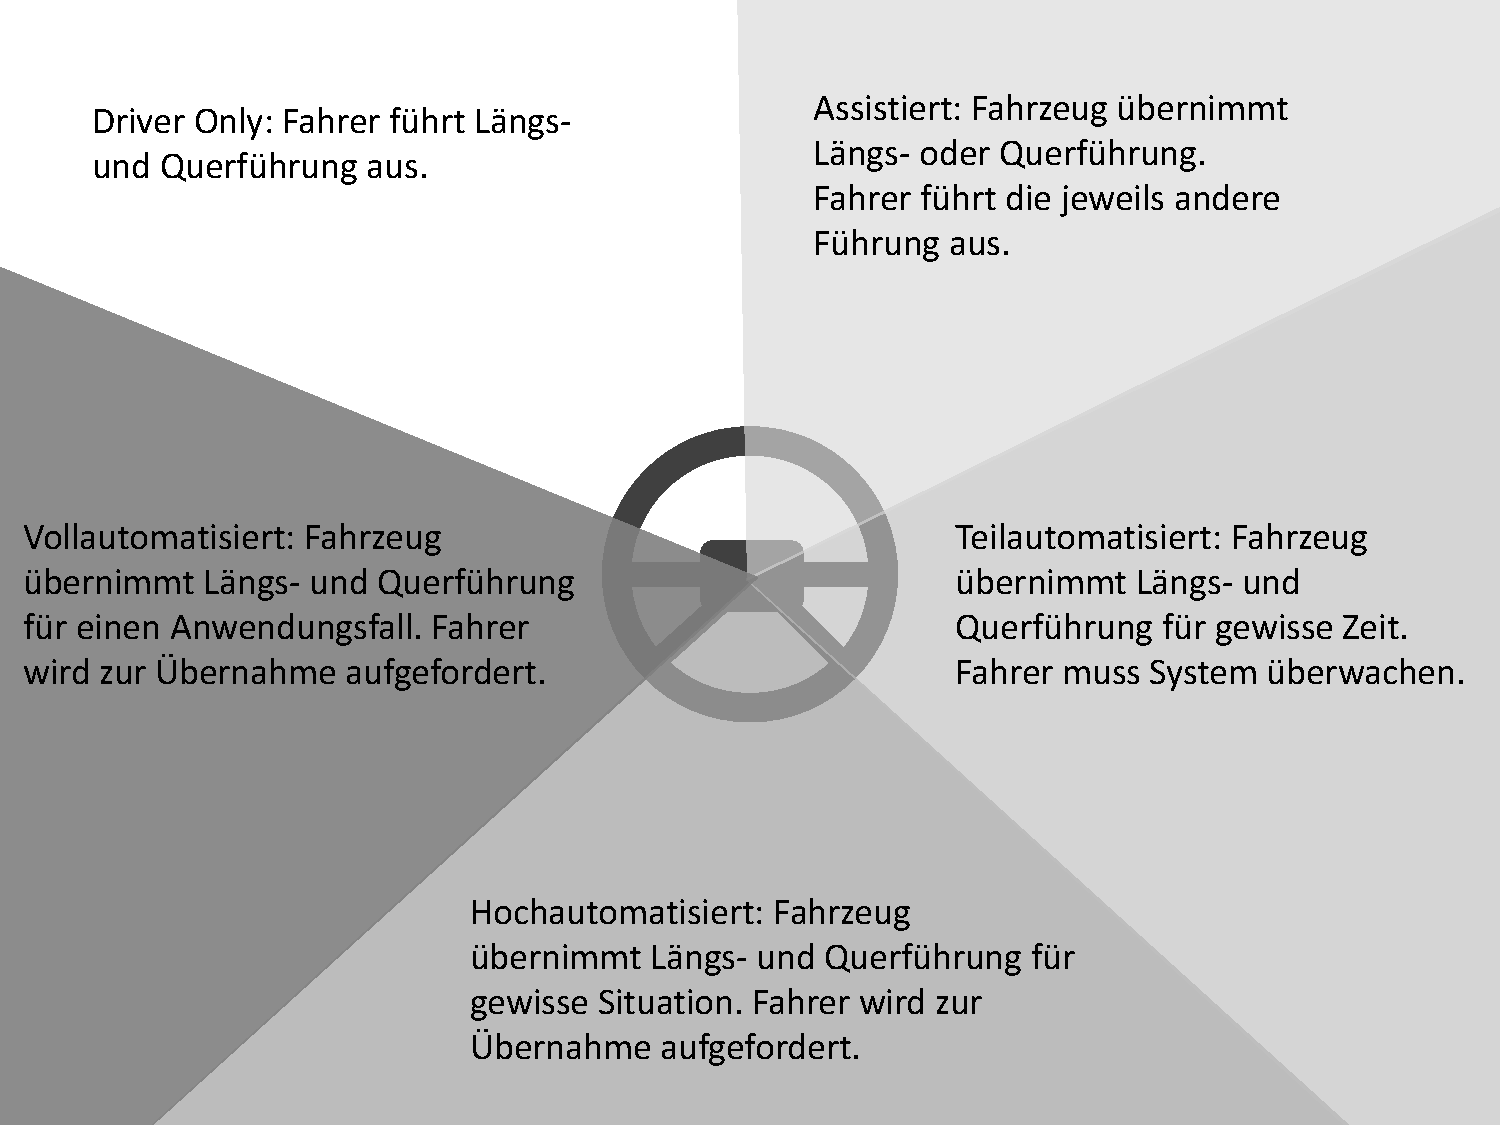
\includegraphics[width=0.8\columnwidth]{pics/Automatisierungsgrade.pdf}%
\caption{Grafische Darstellung der einzelnen Automatisierungsgrade}%
\label{fig:Automatisierungsgrade}%
\end{figure}

Heutzutage werden Serienfahrzeuge mit Sensoren zur Umfelderfassung f�r die Unterst�tzung des Fahrers ausger�stet \cite{Winner.2015}. In Abbildung \ref{fig:Fahrzeugsensoren} ist eine m�gliche Anordnung f�r eine \unit{360}{�}-Wahrnehmung des Fahrzeuges dargestellt. Zu erkennen ist, dass das Long Range Radar und das Lidar in Fahrtrichtung genutzt wird. Dies begr�ndet sich in ihrer hohen Reichweite. So wird ein gro�er Sichtbereich in Fahrtrichtung abgedeckt. Sensoren mit einer geringeren Reichweite werden eingesetzt, um das n�here Umfeld zu beobachten. Hierzu geh�ren das Short Range Radar, die Kamera und der Ultraschall.

\begin{figure}[h]
	\centering
	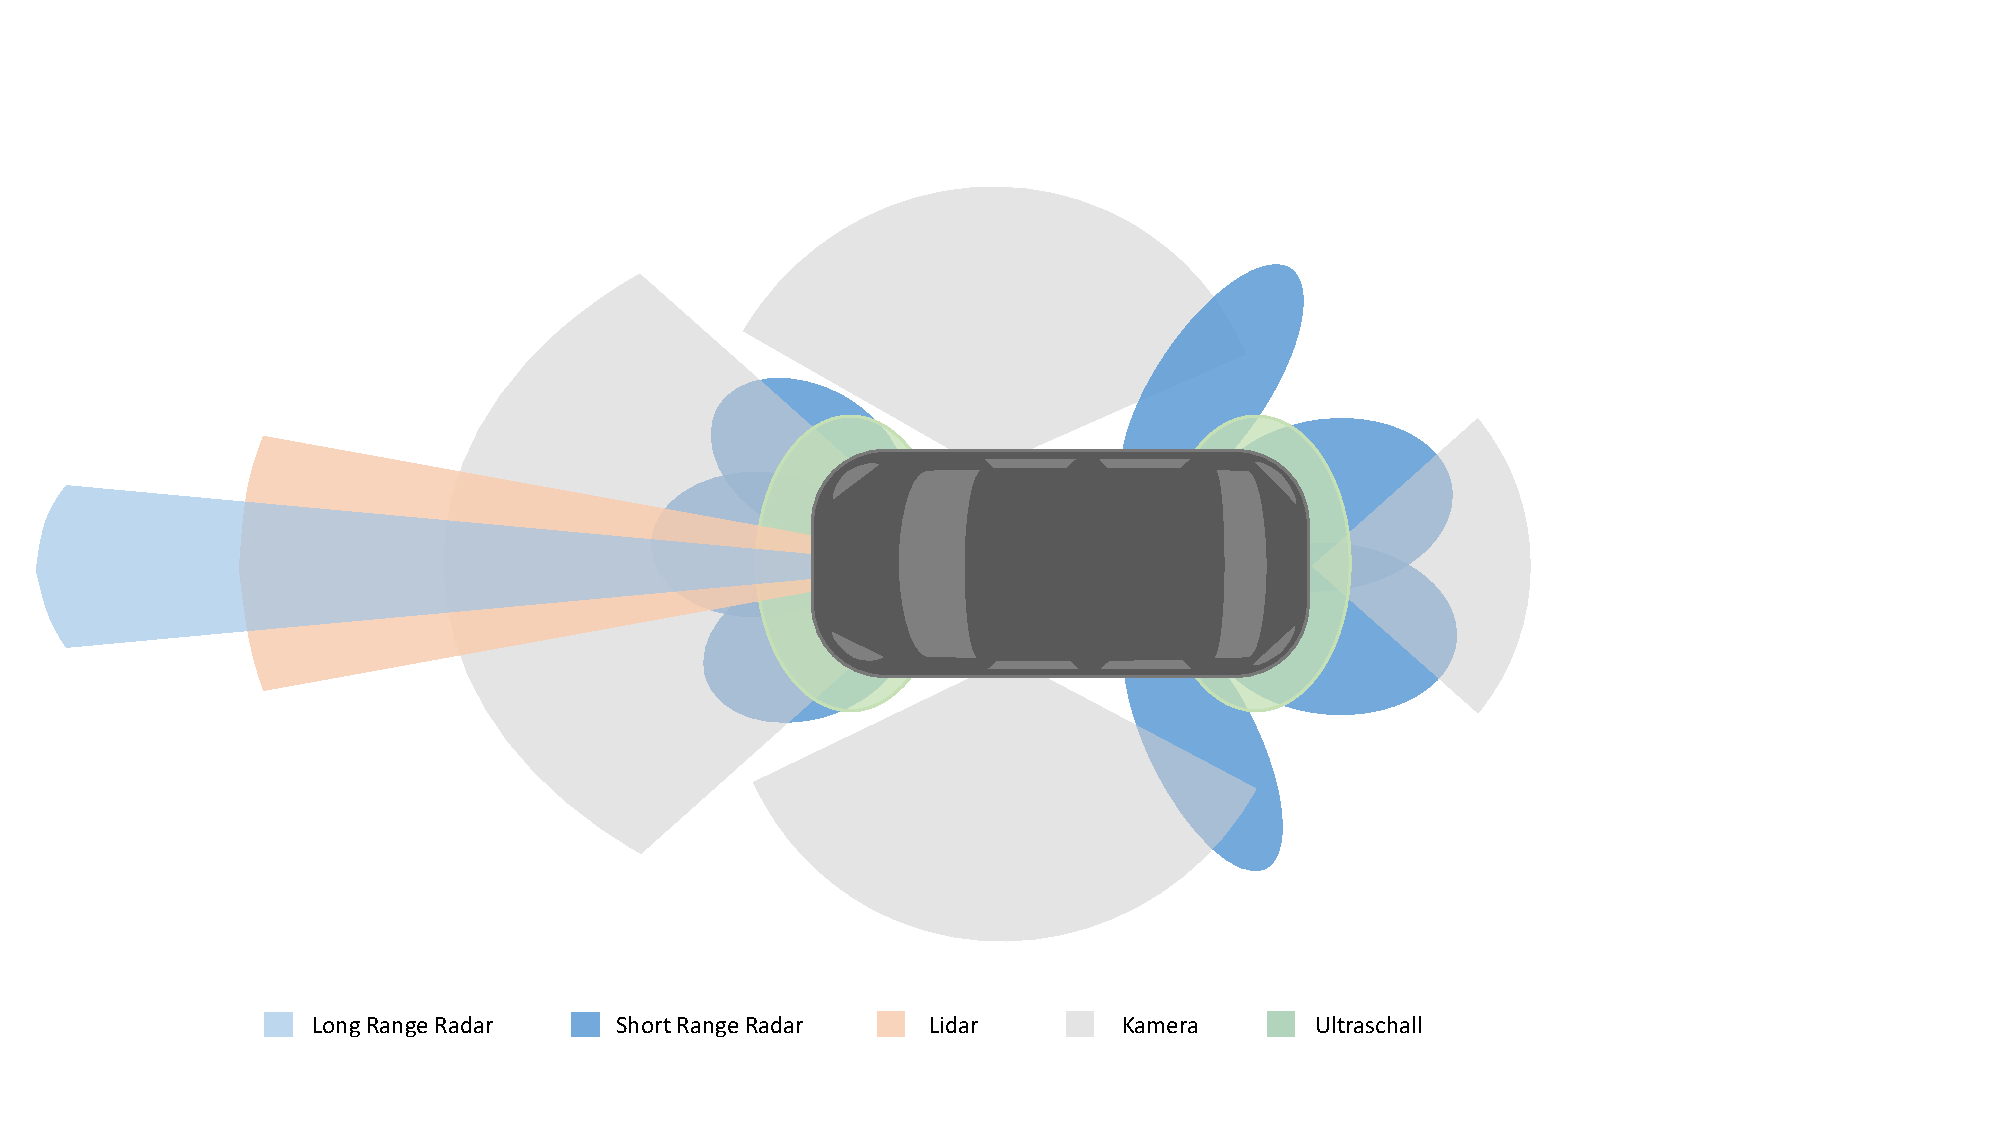
\includegraphics[width=\textwidth,trim={0.5cm 1cm 7.5cm 3cm},clip]{pics/Fahrzeugsensoren.pdf}
	\caption{Beispielhafte Darstellung der Umfelderfassungssensoren am Fahrzeug}
	\label{fig:Fahrzeugsensoren}
\end{figure}

Das Long Range Radar und das Lidar wird im Rahmen von Fahrerassistenzsystemen z.B. f�r ein Adaptive Cruise Control (ACC) genutzt. Zum Teil werden sie au�erdem mit einer Kamera f�r die Fahrstreifenerkennung kombiniert. So kann der Fahrer beispielsweise bei einer Autobahnfahrt entlastet werden. Es wird hierbei eine Wunschgeschwindigkeit eingestellt, die bis zu einer Ann�herung an ein weiteres Fahrzeug gehalten wird. Mit Hilfe der Fahrstreifenerkennung kann au�erdem die Querf�hrung �bernommen werden. Die Sensoren f�r das n�here Umfeld werden unter anderem f�r Spurwechsel-, Toter-Winkel- und Einparkassistenten genutzt. Erstere dienen zur Vermeidung von Unf�llen mit seitlich von Hinten herannahenden oder kreuzenden Verkehrsteilnehmern. Letztere erleichtern das Einparken oder �bernehmen es zum Teil ganz.

Damit Fahrzeuge ohne menschliches Eingreifen zuk�nftig fahren k�nnen, wird viel an der Umfelderfassung geforscht. Eine Auswahl an Arbeiten ist in Tabelle \ref{tab:LitFahrzeug} aufgef�hrt. Zum einen muss das statische Umfeld erfasst werden und zum anderen das dynamische. Zu ersterem geh�ren unter anderem der Verlauf der Fahrstreifen, Kreuzungen und statische Objekte wie Baustellen, Verkehrsschilder oder Br�cken. Alle dynamischen Objekte wie LKWs, PKWs, Fahrradfahrer und Fu�g�nger geh�ren zum dynamischen Umfeld. Auch der Status von Lichtsignalanlagen oder die Witterung geh�ren hierzu. Somit werden z.B. Verfahren erforscht, um mittels Radar Fu�g�nger detektieren zu k�nnen \cite{Ahtiainen.2010}, \cite{Bartsch.2012}. Dies ist aufgrund ihres geringen Querschnittes und der geringen Winkelaufl�sung des Radars schwierig. Des Weiteren werden Verfahren entwickelt, die Infrarotkameras nutzen \cite{Negied.2015}, \cite{Wang.2015}. F�r die Verbesserung der Datenqualit�t wird auch an der Sensordatenfusion gearbeitet \cite{RudiLindl.2009}, \cite{Apatean.2013}.

F�r das vollautomatisierte Fahrzeug spielt neben der Umfeldwahrnehmung die Selbstwahrnehmung und die Selbstlokalisierung eine wichtige Rolle. Bei der Selbstwahrnehmung werden Umfelddaten wie beispielsweise die Witterung genutzt, um die sichere Ausf�hrbarkeit von Handlungsalternativen zu bewerten \cite{Reschka.}. Die Selbstlokalisierung wird f�r den Einsatz von Kartendaten und der Bewertung der Umgebung genutzt. Hierbei werden gemessene Umfeldmerkmale mit Kartenmerkmalen verglichen um das Fahrzeug zu lokalisieren. F�r die Selbstlokalisierung gibt es verschiedene Ans�tze mit unterschiedlichen Kombinationen von Umfelderfassungssensoren mit GPS, Beschleunigungs- und Geschwindigkeitssensoren und digitalen Karten. Einige Ans�tze sind in \cite{Krzikalla2013}, \cite{Schindler.}, \cite{Broggi.2013},\cite{Lundgren.} und \cite{Vivacqua.2017} zu finden.

Ein weiterer Anwendungsfall von Sensoren am Fahrzeug ist die Untersuchung des Verkehrsteilnehmerverhaltens. Einige Vorgehen werden in \cite{Ernst.} und \cite{Bengler.2018} vorgestellt. Mit Hilfe dieser Untersuchungen sollen Algorithmen entwickelt werden, die das Verhalten der Verkehrsteilnehmer absch�tzen. Dies kann schlie�lich f�r die Man�verplanung genutzt werden.


\begin{table}[h]
	\centering
		\begin{tabularx}{\textwidth}{p{2cm}p{2.5cm}Xc}
		\textbf{Quelle} & \textbf{Sensorsetup} & \textbf{Beschreibung} &  \textbf{Jahr}\\ \toprule
		\cite{RudiLindl.2009} & Radar\newline Lidar\newline Kamera & Sensorfusion f�r Fahrerassistenzsysteme mit hohen Anspr�chen  & 2009\\ \midrule
\cite{Perrone.2010} & Stereokamera & Modell zur Datenanalyse von Stereo Kameras  & 2010 \\ \midrule
\cite{Ahtiainen.2010} & 2 x Radar & Erkennen eines Menschen mit Radar  & 2010\\ \midrule
\cite{Bartsch.2012} & Radar & Erkennen eines Menschen mit Radar & 2012\\ \midrule
\cite{Reschka.} &	Radar\newline Lidar	& Nutzt Umgebungsmessungen zur Anpassung des Fahrverhaltens bei beispielsweise Regen &	2012\\ \midrule

\cite{Krzikalla2013} & Lidar \newline GPS & Selbstlokalisierung mit Hilfe von GPS, Laserscanner und digitaler Karte &  2013\\ \midrule
\cite{Yalcin.2013} & Lidar & Positionierung des LIDAR, Fahrbahnbegrenzung erkennen, Objekterkennung  & 2013\\ \midrule
\cite{Apatean.2013} & IR\newline VIS Video & Fusioniert Infrarotkameradaten mit Daten des sichtbaren Spektrums einer Kamera  & 2013\\ \midrule
\cite{Schindler.} & Kamera\newline Lidar\newline GPS & Erzeugen einer Karte mit Hilfe von aktuellen Messdaten, Selbstlokalisierung des Fahrzeugs  & 2013\\ \midrule
\cite{Broggi.2013} &	Lidar\newline Kamera	& KFZe ausger�stet mit Lidar und Kamera, �berlappende Sichtbereiche, autonome Fahrt �ber \unit{13000}{km} durch Europa und Asien	&	2013 \\ \midrule
\cite{Lundgren.} & GPS\newline Gyroscope\newline Kamera\newline Radar & KFZ ausgestattet mit GPS, Gyroscope, Geschwindigkeitsmesser, Kamera, Radar zur Selbstlokalisierung  & 2014\\ \midrule
\cite{Negied.2015} & IR & Literaturauflistung bzgl Erkennung von Menschen mit Infrarotsensor & 2015\\ \midrule
\cite{Wang.2015}   & FIR & stellt einen Filter zur Objekterkennung mit Infrarot vor &  2015\\ \midrule
\cite{Ernst.}	& Lidar	& Nutzt digitale Karte und Lidar zur Extraktion von Verkehrsteilnehmern und bestimmt ihr Verhalten	&	2016\\ \midrule
\cite{Vivacqua.2017} & GPS\newline Gyroscope\newline Kamera & KFZ ausgestattet mit GPS, Gyroscope, Kamera und Laptop zur Selbstlokalisierung & 2017\\ \bottomrule
		\end{tabularx}
	\caption{Einsatz von Sensoren im Fahrzeug}
	\label{tab:LitFahrzeug}
\end{table}

\subsubsection{In der Infrastruktur}
\label{sec:InfraSensor}
In der Infrastruktur werden Umfelderfassungssensoren f�r die Verkehrsbeobachtung genutzt. Die aufgenommenen Daten werden f�r die Analyse der Verhaltensweisen von Verkehrsteilnehmern und zur Unfallforschung genutzt. So k�nnen Verhaltensmuster ermittelt werden, die zu Unf�llen f�hren. Hierbei ist die Interaktion zwischen KFZ bzw. LKW und Fahrrad oder Fu�g�nger interessant \cite{Bengler.2018}. Au�erdem wird der Einfluss der Witterung und der Tageszeit auf das Unfallgeschehen untersucht \cite{J.Ehrlichetal..2009}. Des Weiteren k�nnen Verfahren entwickelt werden, die die Intentionen der Verkehrsteilnehmer vorhersehen k�nnen. F�r die Datenaufnahme werden die Sensoren beispielsweise an Lichtisgnalanlagen montiert \cite{Goldhammer2012}, \cite{Goldhammer.18.09.2013}, \cite{Strigel.}, \cite{KnakeLanghorst.2016}. Au�erdem gibt es mobile Ans�tze f�r die Verkehrs�berwachung, wie z.B. der Einsatz von unbemannten Luftfahrzeugen (ULF) \cite{Kanistras2013}. Der Vorteil hierbei ist der gr��ere Blickwinkel und die M�glichkeit beispielsweise Staus aufzunehmen.

Tabelle \ref{tab:LitInfrastruktur} f�hrt einige Arbeiten auf, die sich mit der Verkehrsbeobachtung besch�ftigen. Am h�ufigsten findet die Kamera hierbei Einsatz, da sie g�nstig sind und eine gro�e Menge an Daten aufnehmen k�nnen. F�r die Bestimmung der Positionen wird sie mit Lidar oder Radar kombiniert. Beispiele f�r m�gliche Versuchsaufbauten sind in den Abbildungen \ref{fig:AIM} und \ref{fig:Ko-PER} dargestellt.

\begin{figure}%
\centering
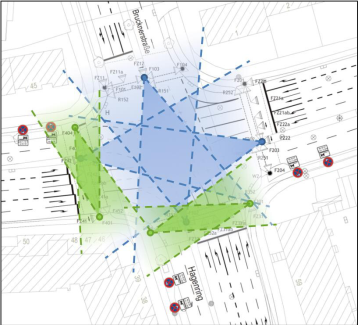
\includegraphics[width=0.7\textwidth,trim={0.3cm 0.5cm 0.5cm 0.5cm},clip]{pics/TestsiteAIM.PNG}%
\caption{Die Forschungskreuzung des Testfeldes AIM in Braunschweig. Blau: Sichtbereich zweier Monokameras kombiniert mit einem \unit{24}{GHz} Radar und einem IR-Blitz. Gr�n: Sichtbereich eines Stereokamerasystems mit einem IR-Blitz \cite{Bengler.2018} \label{fig:AIM}}
\end{figure}

\begin{figure}%
\centering
\subfigure[]{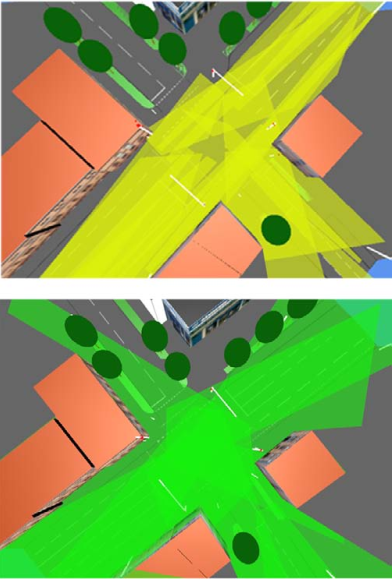
\includegraphics[width=0.4\textwidth,trim={0cm 6.5cm 0cm 0cm},clip]{pics/KooPERTestsite.PNG}}\vspace{10pt}
\subfigure[]{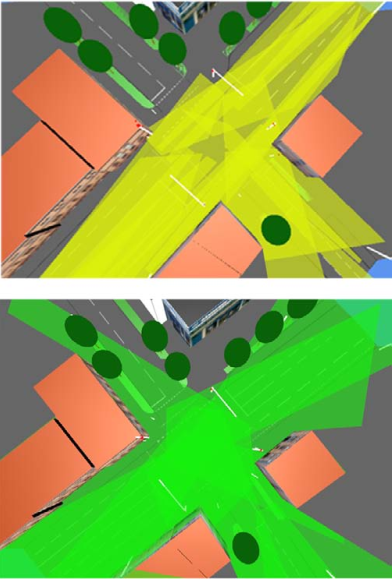
\includegraphics[width=0.4\textwidth,trim={0cm 0cm 0cm 6.5cm},clip]{pics/KooPERTestsite.PNG}}%
\caption{Sensoraufbau der Ko-PER Kreuzungen in Aschaffenburg. Gelb: Sichtbereich der Laserscanner. Gr�n: Sichtbereich der Kameras \cite{Goldhammer2012} \label{fig:Ko-PER}}
\end{figure}

Neben der Verhaltensanalyse der Verkehrsteilnehmer soll der Einsatz von Umfelderfassungssensoren der Steuerung des Verkehrs dienen. Hierf�r werden die aufgenommenen Daten mittels Car2X-Kommunikation an die Fahrzeuge �bermittelt. Welche ihrerseits ihre Daten an die Infrastruktur senden. Dies erm�glicht eine einergie- und verkehrseffizientere Routenplanung und eine Reduzierung von Unf�llen.

\begin{table}
	\centering
		\begin{tabularx}{\textwidth}{p{2cm}p{2.5cm}Xc}
		\textbf{Quelle} & \textbf{Sensorsetup} & \textbf{Beschreibung} &  \textbf{Jahr}\\ \toprule
			\cite{J.Ehrlichetal..2009} & Kamera\newline Lidar \newline IR & CCTV, Laserscanner, IR zur Verkehrs- und Umweltbeobachtung (Bestimmung der Witterung, Tageszeit) &  2009\\ \midrule
\cite{Meissner.} & Lidar & Einsatz und Modellierung von Laserscannern an Kreuzungen &  2012\\ \midrule
\cite{Goldhammer2012} & Lidar\newline Kamera & Beschreibt den Versuchsaufbau an einer Kreuzung zur Beobachtung des Verkehrs &  2012\\ \midrule
\cite{Hospedales.2012} & Kamera & Vergleicht Algorithmen zur Verhaltenserkennung von Verkehrsobjekten in Kameradaten &  2012\\ \midrule
\cite{Goldhammer.18.09.2013} & Lidar\newline Kamera & Einsatz von Sensoren an einer Kreuzung (Anbauorte) &  2013\\ \midrule
\cite{EliasStrigel2013} & Lidar\newline Kamera & Einsatz von Kameras und Laserscanner an einer Kreuzung zur Beobachtung des Verkehrs  & 2013\\ \midrule
\cite{Kanistras2013} & Kamera\newline Radar &	�berblick von verschiedenen Studien, die ULFs zur Verkehrs�berwachung nutzen. Ausgestattet mit Kamera/Radar &	2013\\ \midrule
\cite{Strigel.} & Lidar\newline Kamera & Beschreibt den Versuchsaufbau an einer Kreuzung zur Beobachtung des Verkehrs & 2014\\ \midrule
\cite{Jodoin.} & Kamera & Stellt einen Algorithmus zum Objekttracking f�r die Bildverarbeitung vor, der an unterschiedlichen Kreuzungen getestet wurde &  2014\\ \midrule
\cite{DatondjiSokemiReneEmmanuel.2016} & Kamera & Listet und diskutiert Ans�tze zur Verkehrsbeobachtung an Kreuzungen &  2016\\ \midrule
\cite{KnakeLanghorst.2016} & Kamera\newline IR\newline Radar & Stellt die Forschungsplatform AIM zur Untersuchung des Verkehrs vor &  2016\\ \midrule
\cite{Shirazi.2017} & GPS\newline Radar\newline Lidar\newline Kamera & Vergleicht verschiedene Ans�tze der Verkehrsbeobachtung und Analyse & 2016\\ \midrule
\cite{Bengler.2018} & Kamera\newline IR\newline Radar & Untersuchung von Konflikten zwischen Fahrradfahrern und motorisierten Fahrzeugen &  2017\\\midrule
\cite{Garcia2018} & Radar & Stellt \unit{76-81}{GHz} Radar zur Verkehrs�berwachung vor &  2018\\ \bottomrule
		\end{tabularx}
	\caption{Einsatz von Sensoren in der Infrastruktur}
	\label{tab:LitInfrastruktur}
\end{table}

\section{Anforderungen an das Simulations-Tool}
\label{chap:Anforderungen}
Kapitel\,\ref{chap:Einsatz} stellte einige bestehende Sensorkonfigurationen f�r Fahrzeuge und der Infrastruktur vor. F�r die Analyse dieser Konfigurationen und Auslegung zuk�nftiger Sensorkonzepte soll ein Simulations-Tool erstellt werden. Daf�r werden im folgenden Kapitel Anforderungen an ein entsprechendes Tool ausgearbeitet. Eine Auflistung der Anforderungen schlie�t das Kapitel ab.

\subsection{Komponenten des Simulations-Tools}
F�r die Analyse von Sensorkonfigurationen m�ssen neben den zu bewertenden Sensoren auch die Umgebung und die Objekte, d.h. die Verkehrsteilnehmer, abgebildet werden. Die Abh�ngigkeiten dieser drei Komponenten sind in Abbildung\,\ref{pic:Anforderungen} dargestellt. Die gr�nen Pfeile geben an, dass die Sensoren in der Umgebung und an den Objekten positioniert werden. Au�erdem sind die Objekte in der Umgebung platziert. Der Einfluss der Umgebung und der Objekte auf die Sensoren ist durch die roten Pfeile dargestellt.
\begin{figure}[hbtp]
\centering
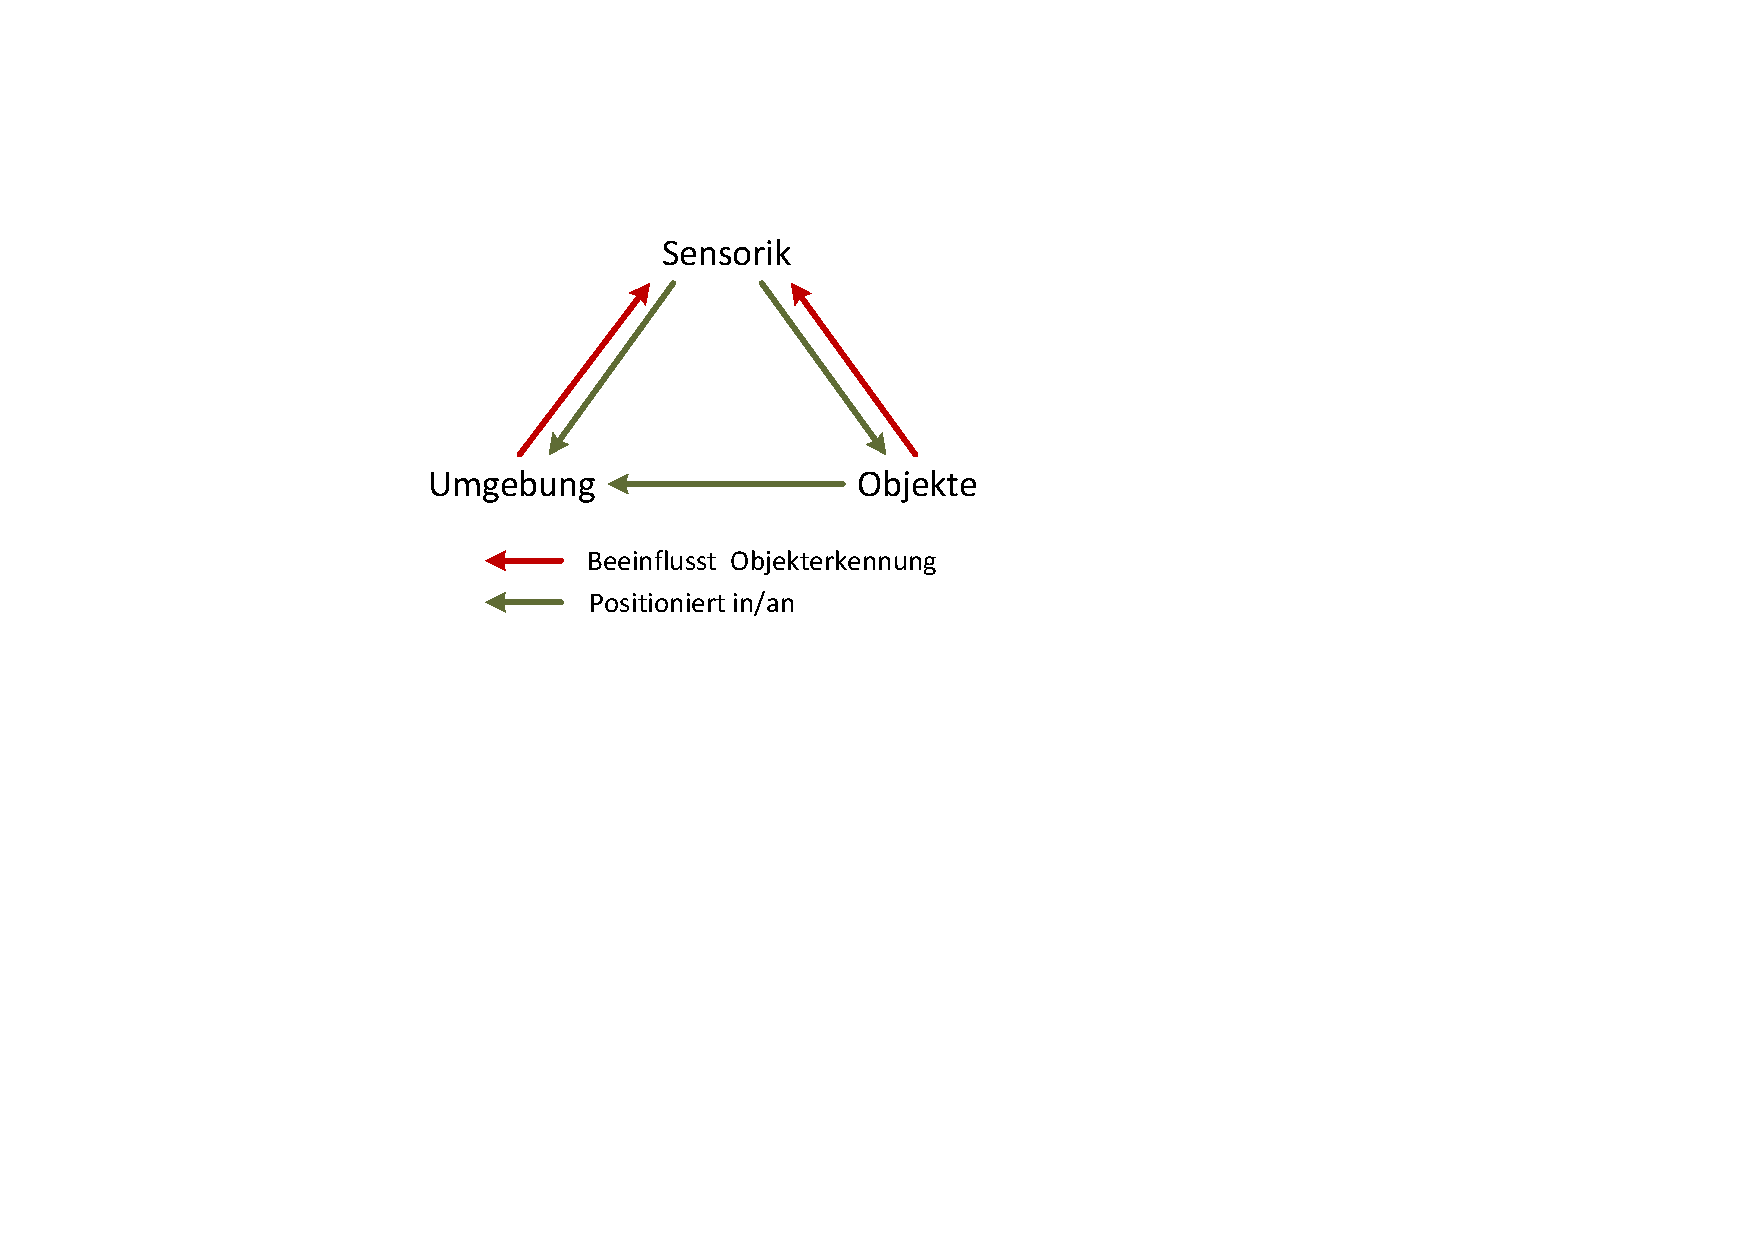
\includegraphics[width=0.7\columnwidth,trim={6.5cm 10.5cm 12cm 4cm},clip]{pics/Anforderungen.pdf}%
\caption{Komponenten des Simulations-Tools}%
\label{pic:Anforderungen}%
\end{figure}

\subsubsection{Sensoren}
\label{sec:AnfSen}
Wie schon in Kapitel\,\ref{chap:Grundlagen} dargestellt, existieren verschiedene Sensortypen zur Umfelderfassung. Die Eigenschaften dieser Typen m�ssen f�r das Tool modelliert werden. Wesentliche Merkmale sind das Sichtfeld, bestehend aus horizontalem und vertikalem �ffnungswinkel $\phi$ und der Reichweite $R_{max}$, und die Latenz und die Genauigkeit der Messung. Des Weiteren m�ssen die Einfl�sse auf die Messung, wie die Witterung und die Lichtverh�ltnisse, ber�cksichtigt werden.

F�r die Bewertung von Sensorkonfigurationen muss dem Benutzer erm�glicht werden, zwischen verschiedenen Sensoren zu w�hlen. Diese muss er au�erdem an den Objekten und in der Umgebung positionieren und ausrichten k�nnen. Des Weiteren sollte ihm erm�glicht werden, individuelle Parameter wie die Latenz der Datenauswertung oder die Objekterkennungswahrscheinlichkeit seines Objekterkennungsalgorithmus anzugeben.

\subsubsection{Objekte}
\label{sec:AnfObj}
Die Verkehrsteilnehmer werden in der Verkehrstechnik als Objekte bezeichnet. Sie werden in folgende Typen unterschieden: \ac{Pkw}, \ac{Lkw}, motorisierte und unmotorisierte Zweir�der und Fu�g�nger.

F�r den automatisierten Verkehr muss, wie schon in Abschnitt \ref{sec:KFZSensor} angef�hrt, das statische und dynamische Umfeld erfasst werden. Mit Hilfe des Simulations-Tools soll �berpr�ft werden k�nnen, wo und wie gut die Objekte erfasst werden. Daf�r muss das Tool alle relevanten Eigenschaften der Objekte abbilden. Dazu z�hlen die Gr��e, die Bewegungsrichtung und die Geschwindigkeit.

Zur Analyse muss der Benutzer Objekte in einer Szene platzieren k�nnen. Au�erdem sollte er den Objekttyp ausw�hlen und die Bewegungsrichtung sowie die Geschwindigkeit bestimmen k�nnen.

\subsubsection{Umgebung}
\label{sec:AnfUmg}
Zur Erzeugung von Use-Cases wird eine Auswahl von verschiedenen Stra�enf�hrungen ben�tigt. Dazu geh�ren verschiedene Kreuzungs- und Stra�entypen ausgestattet, mit Verkehrsschildern und/oder Lichtsignalanlagen. Dar�ber hinaus sollte dem Benutzer erm�glicht werden, reale Kartendaten zu laden. Damit w�re es m�glich, bestimmte Verkehrsknotenpunkte oder auch ganze St�dte im Bezug auf Sensorkonfigurationen zu analysieren.

Weitere Umgebungsbestandteile, die f�r das Tool modelliert werden m�ssen, sind sichteinschr�nkende Elemente wie H�user und B�ume. Auch die Tageszeit bzw. die Lichtverh�ltnisse und die Witterung m�ssen modelliert werden, um deren Einfluss auf die Sensoren ber�cksichtigen zu k�nnen. Daf�r sollte dem Benutzer erm�glicht werden, diese einzustellen.

\subsubsection{Auswertung}
\label{sec:AnfAusw}
Mit Hilfe der modellierten Eigenschaften der Sensoren, der Objekte und der Umgebung k�nnen Use-Cases ausgewertet werden. Daf�r muss zun�chst bestimmt werden, welche Objekte sich innerhalb des Sensorsichtfeldes befinden. Unter Ber�cksichtigung der Einfl�sse muss daraufhin ermittelt werden mit welcher Wahrscheinlichkeit jedes Objekt erkannt wird. Des Weiteren muss die Latenz und Genauigkeit der Erkennung bestimmt werden. Diese Werte m�ssen schlie�lich an den Benutzer ausgegeben werden.

Da in der Regel mehr als ein Sensor an einem Objekt bzw. an der Infrastruktur verbaut wird, muss bei der Auswertung der Objekterkennung auch die Sensordatenfusion ber�cksichtigt werden. Zus�tzlich k�nnen die Daten per \acs{C2X}-Kommunikation weitergeleitet werden, was ebenfalls die Werte der Objekterkennung beeinflusst.

Neben der statischen Auswertung einzelner Momentaufnahmen sollte des Weiteren eine zeitliche Auswertung m�glich sein. Dadurch k�nnen schlie�lich auch zeitliche Abh�ngigkeiten ber�cksichtigt werden.

F�r das bessere Verst�ndnis des Benutzers sollte die Szene au�erdem grafisch dargestellt werden. Hierbei sollte die Option bestehen einzelne Szenenelemente zu vergr��ern. So k�nnen St�dte und Knotenpunkte im Ganzen oder Konfliktszenen im Detail betrachtet werden.

Abschlie�end muss der Benutzer die erzeugte Szene speichern und laden k�nnen. Dadurch kann eine Reproduzierbarkeit gew�hrleistet werden.

\subsection{Anforderungsliste}
\label{sec:Anforderungsliste}
Aus den zuvor erarbeiteten Punkten kann schlie�lich eine Anforderungsliste erstellt werden. Dabei k�nnen die Anforderungen in die vier Komponenten "`Sensoren"', "`Objekte"', "`Umgebung"' und "`Auswertung"' eingeteilt werden. In Tabelle\,\ref{tab:Anforderungen} befindet sich diese Auflistung.

\begin{tabularx}{\textwidth}{lX}
\caption{Anforderungen an die Implementierung}
	\label{tab:Anforderungen}\\\toprule
\textbf{Nr} & \textbf{Anforderung} \\ \midrule\endfirsthead
\caption*{Anforderungen an die Implementierung}
	\label{tab:Anforderungen}\\\toprule
\textbf{Nr} & \textbf{Anforderung} \\ \midrule\endhead
\midrule\endfoot 
\bottomrule\endlastfoot
\textbf{S} & \textbf{Sensoren}\\
S1 & Verschiedene Sensortypen m�ssen gew�hlt werden k�nnen\\
S2 & Das Sichtfeld der Sensoren muss gew�hlt werden k�nnen\\
S3 & Sensoren m�ssen positioniert werden k�nnen\\
S4 & Sensoren m�ssen ausgerichtet werden k�nnen\\
S5 & Der Einfluss der Witterung auf die Messung muss ber�cksichtigt werden\\
S6 & Der Einfluss der Lichtverh�ltnisse auf die Messung muss ber�cksichtigt werden\\\midrule

\textbf{O} & \textbf{Objekte}\\
O1 & Objekte m�ssen platziert werden k�nnen\\
O2 & Verschiedene Objekttypen m�ssen den Objekten zugeordnet werden k�nnen\\
O3 & Jedem Objekt muss eine Bewegungsrichtung zugeordnet werden k�nnen\\
O4 & Jedem Objekt muss eine Geschwindigkeit zugeordnet werden k�nnen\\\midrule

\textbf{U} & \textbf{Umgebung}\\		
U1 & Eine Stra�enf�hrung muss ausgew�hlt werden k�nnen \\ 
U2 & Infrastrukturelemente m�ssen eingef�gt werden k�nnen\\
U3 & Die Witterung muss gew�hlt werden k�nnen\\
U4 & Die Tageszeit muss gew�hlt werden k�nnen\\
\midrule

\textbf{A} & \textbf{Auswertung}\\
A1 & Objekte im Sichtfeld m�ssen erkannt werden\\
A2 & Die Erkennungswahrscheinlichkeit des Objekterkennungsalgorithmus muss gew�hlt werden k�nnen\\
A3 & Der Abstand zum Objekt muss bestimmt werden\\
A4 & Der Abstand muss die Objekterkennung beeinflussen\\
A5 & Die Objekterkennungswahrscheinlichkeit muss bestimmt werden\\
A6 & Die Objekterkennungswahrscheinlichkeit muss ausgegeben werden\\
A7 & Die Geschwindigkeit des Objektes muss bestimmt werden k�nnen\\
A8 & Die Genauigkeit der Messung muss ausgegeben werden\\
A9 & Die Sensorfusion muss ber�cksichtigt werden\\
A10 & Die ermittelte Objektposition soll ausgegeben werden\\
A11 & Die Latenz der Messung muss ber�cksichtigt werden\\
A12 & Die Latenz der Datenverarbeitung muss ber�cksichtigt werden\\
A13 & Die Latenz, bis das Objekt erkannt ist, muss ausgegeben werden\\
A14 & Eine zeitliche Auswertung muss m�glich sein\\
A15 & Die Szene muss grafisch dargestellt werden k�nnen\\
A16 & Es muss die M�glichkeit des Zoomens bestehen\\
A17 & Die Szene muss gespeichert werden k�nnen\\
A18 & Szenen m�ssen geladen werden k�nnen\\\bottomrule
\end{tabularx}


	
		%\begin{itemize}
			%\item FoV (�ffungswinkel, Reichweite)
			%\item Datenqualit�t (Aufl�sung Genauigkeit, Messdauer)
			%\item Arbeitsfrequenz
			%\item Umwelteinfl�sse (Witterung, Tag/Nacht, Temperatur)
			%\item Ma�e (Gr��e, Gewicht)
			%\item Schnittstellen
		%\end{itemize}

\section{Simulations-Tool}
\label{chap:Software-Tool}
%Im folgenden Kapitel werden zun�chst die Anforderungen an ein Werkzeug zur Systemkonzeptbewertung von infrastrukturellen Umfelderfassungsl�sungen erl�utert. Dieses Werkzeug soll als Software umgesetzt werden, welche anschlie�end vorgestellt wird. Ziel ist es, mit Hilfe dieses Tools infrastrukturelle Umfelderfassungsl�sungen in Hinblick auf das automatisierte Fahren zu bewerten. Somit best�nde unter anderem die M�glichkeit, Stadtverwaltungen potenzielle Umfelderfassungsl�sungen f�r beispielsweise Verkehrsknotenpunkte aufzuzeigen, mit denen das automatisierte Fahren gef�rdert werden k�nnte.

Nachdem in Kapitel\,\ref{chap:Anforderungen} die Anforderungen spezifiziert worden sind, wird im folgenden Kapitel die Umsetzung dieser Anforderungen in Matlab vorgestellt. Zun�chst werden hierf�r die Benutzeroberfl�che und der Programmablauf erl�utert. Anschlie�end wird genauer auf die Implementierung der Funktionen eingegangen.

\subsection{Benutzeroberfl�che}
\label{sec:GUI}
%Links: Darstellung der Szene\\
%Rechts oben: Definieren der Szenenparameter\\
%Rechts mittig: Eingabe der sensorspezifischen Einfl�sse auf die Objekterkennung\\
%Rechts unten: Ausgabe der Auswertung\\

Abbildung\,\ref{fig:GUI} zeigt die grafische Benutzeroberfl�che des Programms. In der linken H�lfte des Fensters wird die Szene visualisiert. Die Parameter hierf�r definiert der Benutzer mit dem Panel "`Szene erstellen"' rechts oben im Fenster (vgl. Abbildung\,\ref{fig:Szene}). Ein Dropdown-Menu erm�glicht die Auswahl der Stra�enf�hrung (U1). Darunter wird die Anzahl der zu platzierenden Objekte in einem Eingabefeld angegeben. Die Auswahl der Tageszeit wird durch die Radiobuttons Tag und Nacht, die darunter platziert sind, realisiert (U4). Die Standardeinstellung ist "`Tag"'. Auf der rechten Seite des Panels "`Szene erstellen"' besteht die M�glichkeit, die Witterung zu ver�ndern (U3). Hierf�r kann der Benutzer zun�chst zwischen "`Trocken"', "`Nebel"' und "`Regen"' w�hlen. Bei Nebel muss der Benutzer noch eine Sichtweite im nebenstehenden Eingabefeld eintragen. Der Standardwert ist \unit[100]{m}. Wenn Regen ausgew�hlt ist, ben�tigt das Programm eine Regenrate, die im Eingabefeld neben "`Regen"' angegeben wird. Als Voreinstellung wird eine Regenrate von \unitfrac[2.5]{mm}{h} angenommen. 

\begin{figure}[hbtp]%
\centering
\subfigure[][Gesamtansicht der Benutzeroberfl�che\label{fig:GUI}]{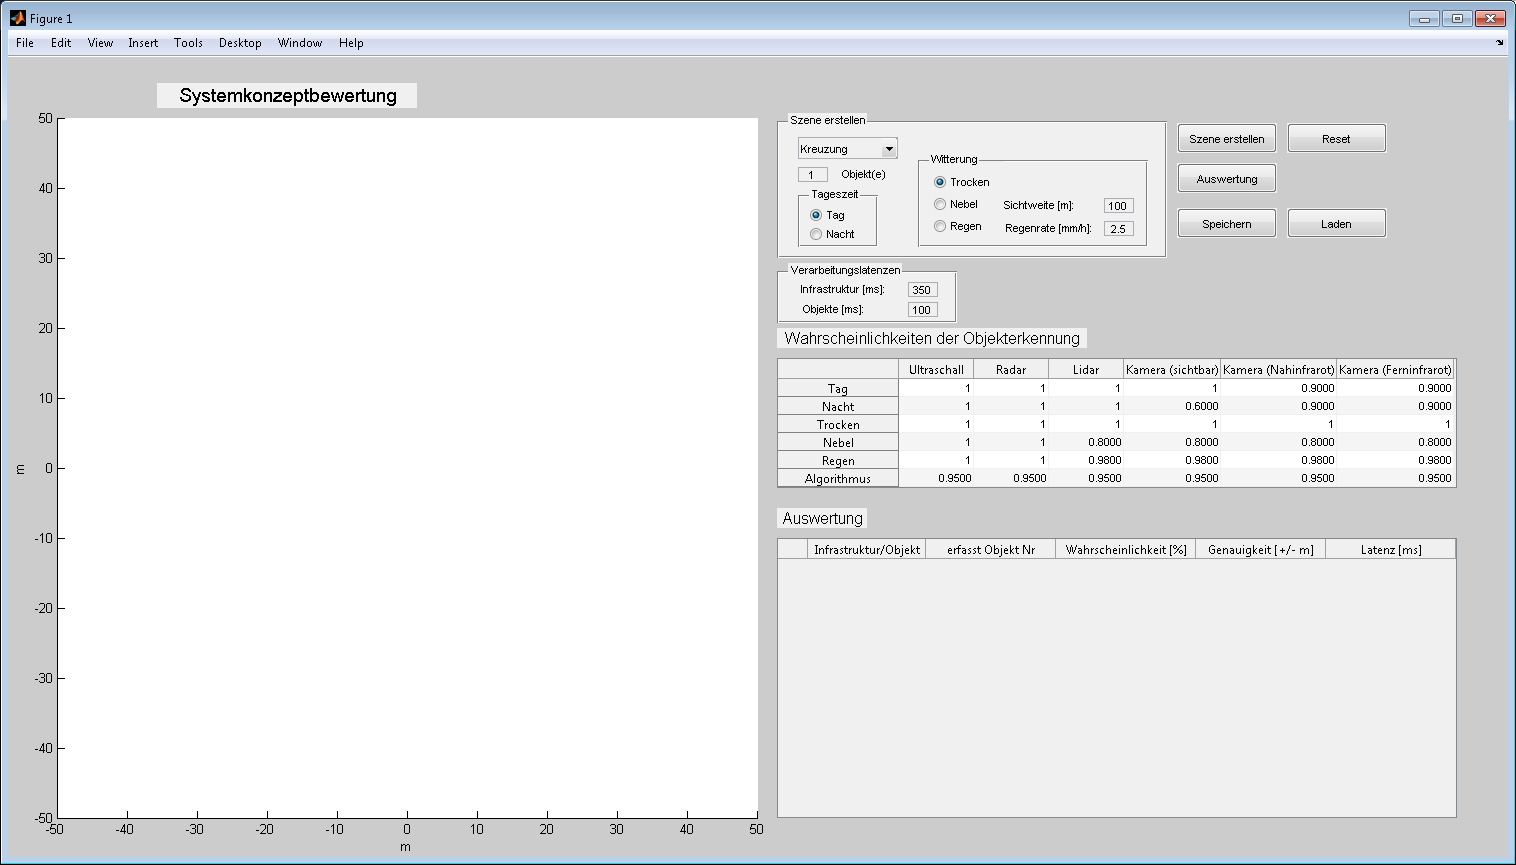
\includegraphics[width=\textwidth]{pics/Tool-GUI.png}}\quad%
\subfigure[][Panel: Szene erstellen\label{fig:Szene}]{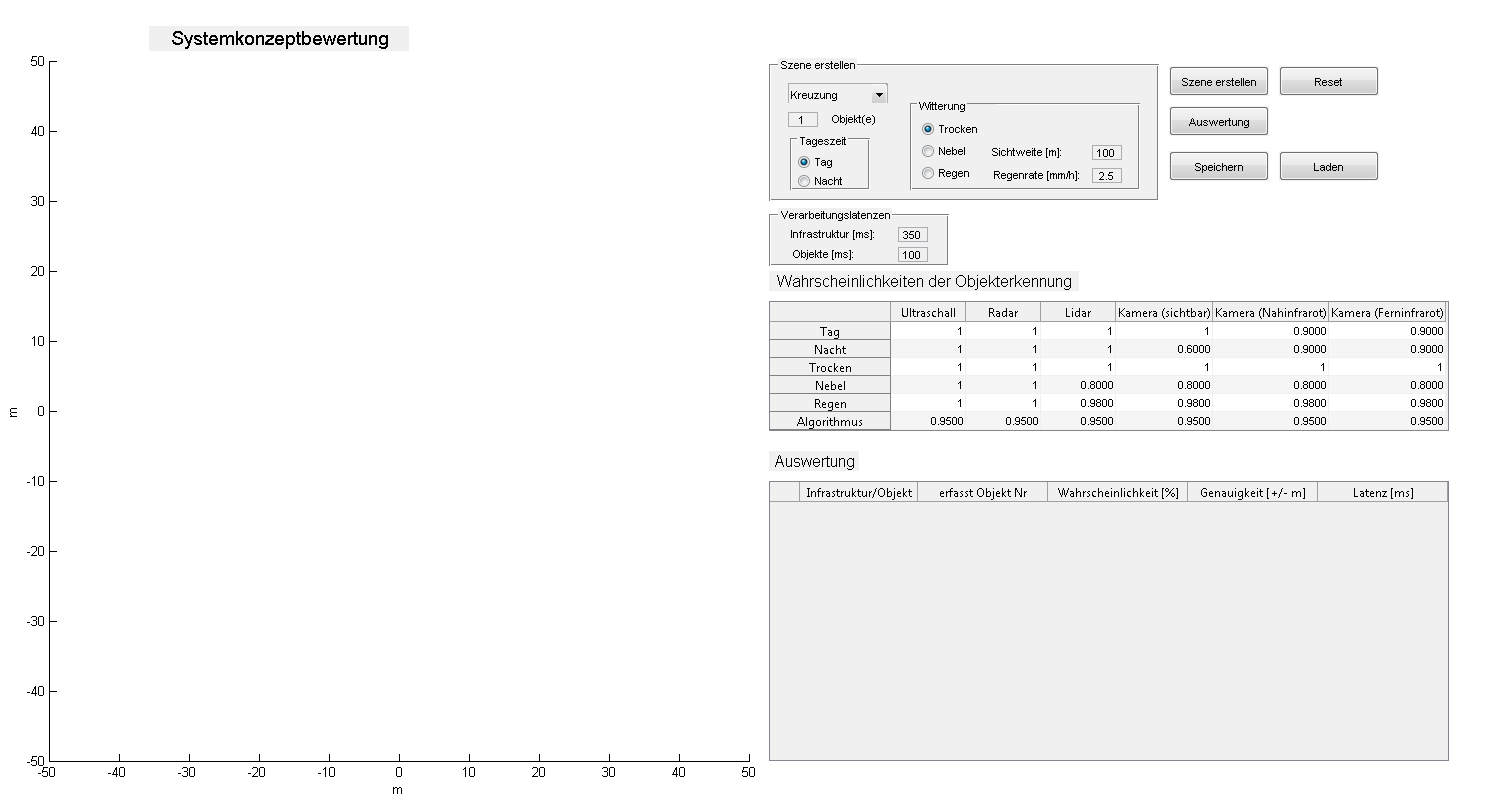
\includegraphics[width=0.55\textwidth,trim={20cm 15.8cm 9cm 1.5cm},clip]{pics/Tool-GUI2.png}}\quad%
\subfigure[][Panel: Verarbeitungslatenzen\label{fig:Latenzen}]{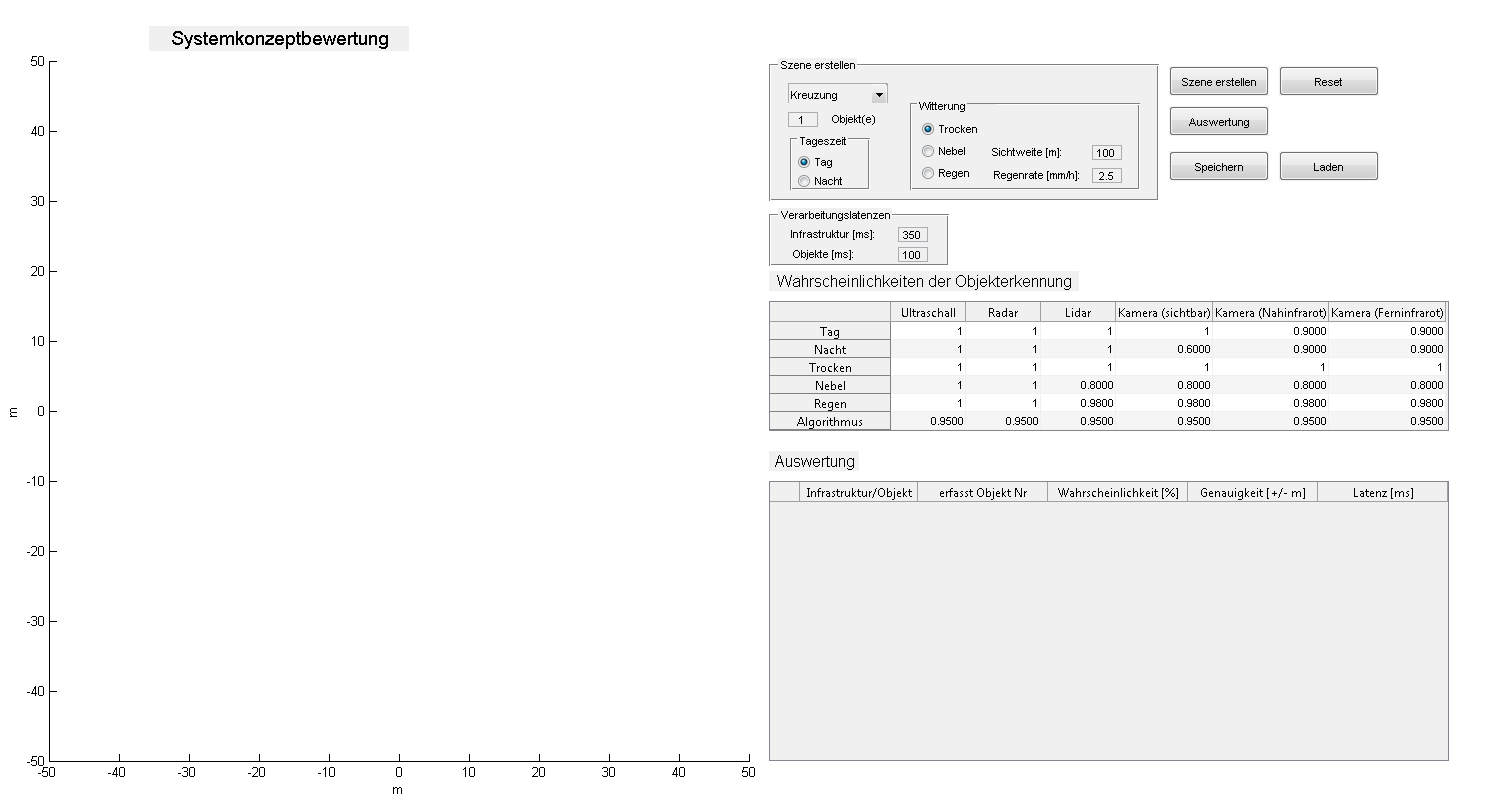
\includegraphics[width=0.35\textwidth,trim={20cm 14cm 14.6cm 5.5cm},clip]{pics/Tool-GUI2.png}}\\%
\subfigure[][Tabelle mit Wahrscheinlichkeiten f�r die Einfl�sse der Objekterkennung\label{fig:TabWahr}]{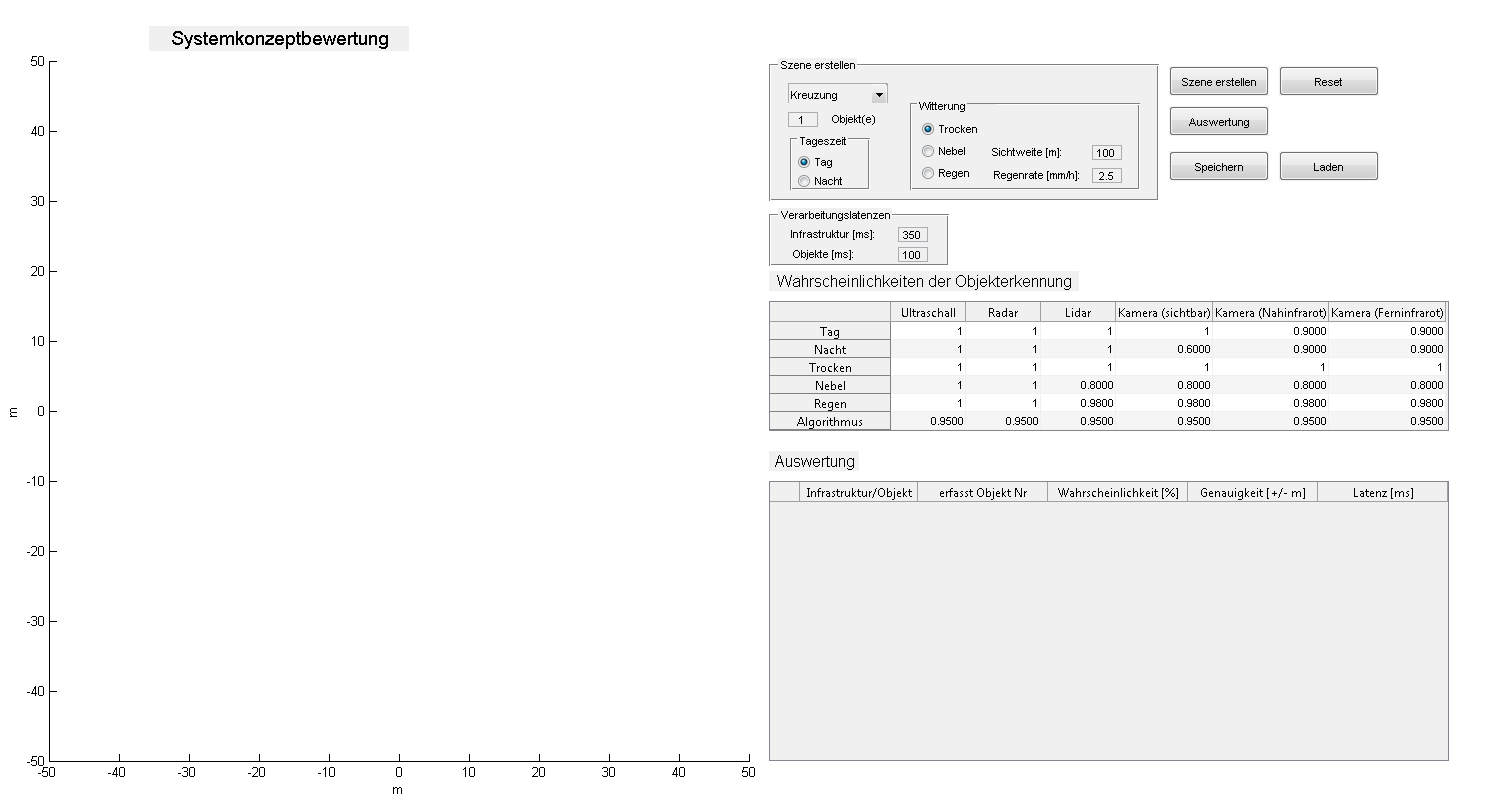
\includegraphics[width=\textwidth,trim={20cm 9.5cm 1cm 7.9cm},clip]{pics/Tool-GUI2.png}}
\caption{Grafische Benutzeroberfl�che des Software-Tools}%%
\end{figure}

Rechts neben dem Panel "`Szene erstellen"' sind f�nf Buttons: "`Szene erstellen"', "`Reset"', "`Auswertung"', "`Speichern"', "`Laden"'. Mit ersterem wird in der linken Bildh�lfte schlie�lich die Szene gezeichnet (A15). Mit dem "`Reset"'-Button wird das Programm wieder auf die Standardeinstellungen zur�ckgestellt. Nachdem die Szene erstellt worden ist, kann mit dem Button "`Auswertung"' die Szene ausgewertet werden. Daraufhin wird die Objekterkennung durchgef�hrt und unten rechts die Tabelle gef�llt (A6, A8, A13). Mit dem Button "`Speichern"' werden alle Variablen gespeichert (A17). Diese k�nnen mit dem Button "`Laden"' zu einem sp�teren Zeitpunkt wieder aufgerufen werden (A18).

Unter dem Panel "`Szene erstellen"' sind Eingabefelder f�r die Angabe von Werten f�r die Verarbeitungslatenzen der Objekte und der Infrastruktur (A12), siehe Abbildung\,\ref{fig:Latenzen}. F�r die Infrastruktur ist standardm��ig \unit[350]{ms} und f�r die Objektlatenz \unit[100]{ms} eingetragen. In der Tabelle darunter sind die sensorspezifischen Wahrscheinlichkeiten der Objekterkennung aufgelistet, siehe Abbildung\,\ref{fig:TabWahr}. Die Eintr�ge der Tabelle kann der Benutzer anpassen (S5, S6, A2). 

\subsection{Programmablauf}
Der Programmablauf ist in Abbildung\,\ref{fig:Programmablauf} als Flussdiagramm dargestellt. Mit Programmstart wird die Benutzeroberfl�che ge�ffnet. Jetzt kann der Benutzer die Szene mit Hilfe des Panels "`Szene erstellen"' definieren. Nach Bet�tigen des Buttons "`Szene erstellen"' wird die Stra�enf�hrung in der linken Fensterh�lfte gezeichnet (A15).

\begin{figure}[hbtp]%
\centering
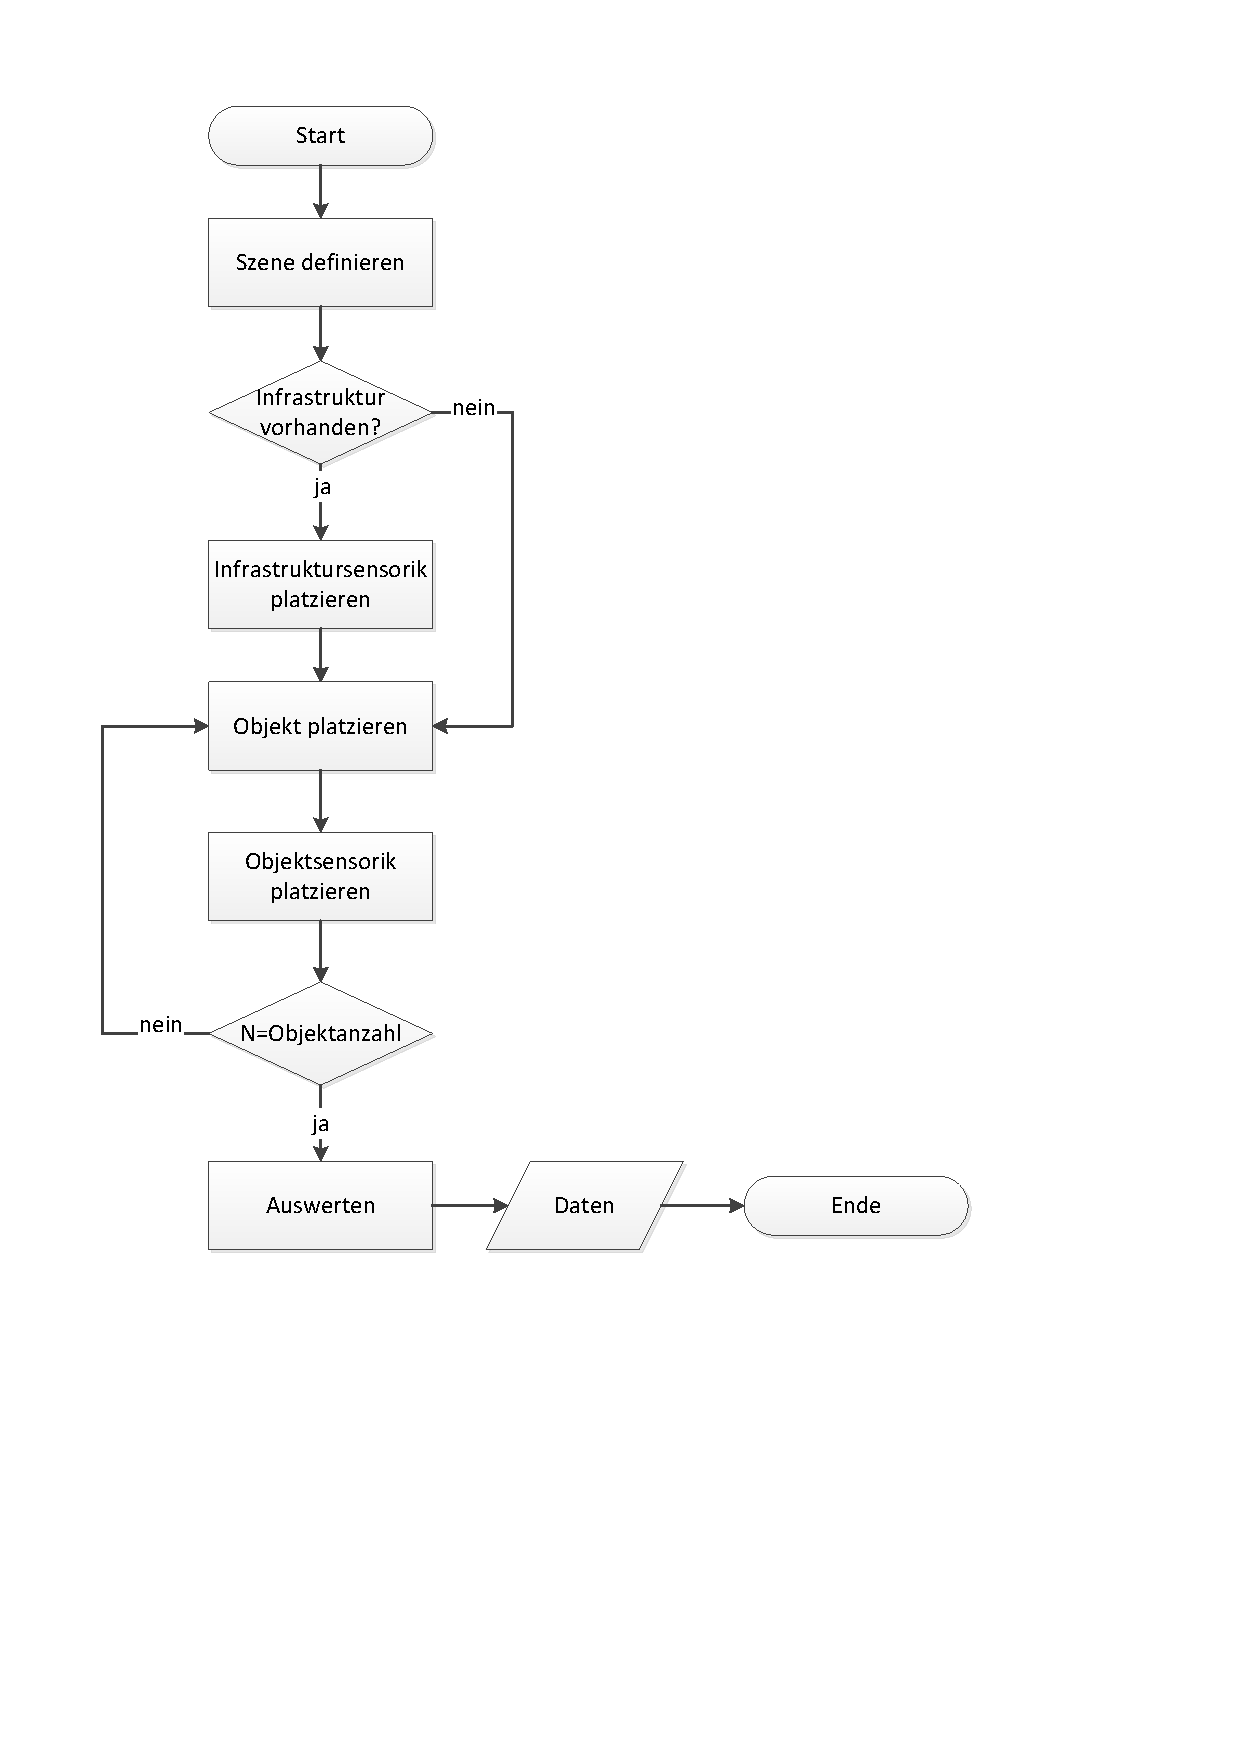
\includegraphics[width=0.85\columnwidth,trim={1cm 8cm 4cm 1.5cm},clip]{pics/Programmablauf.pdf}%
\caption{Flussdiagramm des Programmablaufs}%
\label{fig:Programmablauf}%
\end{figure}
%\newpage

Wenn Infrastrukturelemente in der ausgew�hlten Stra�enf�hrung vorhanden sind (U2), wird der Benutzer zun�chst aufgefordert, diese mit Sensorik auszustatten. Hierf�r wird nacheinander f�r jedes Element zun�chst die Sensoranzahl abgefragt und der Benutzer wird aufgefordert, einen Sensor ausw�hlen (S.1, S.2) und dessen Position (S3) und Ausrichtung (S4) am aktuellen Infrastrukturelement anzugeben. Wenn keine Infrastrukturelemente in der ausgew�hlten Stra�enf�hrung existieren, k�nnen keine Infrastruktursensoren platziert werden.

Anschlie�end wird der Benutzer aufgefordert, die Objekte zu platzieren (O1). Dies geschieht per Mausklick innerhalb der Stra�enf�hrung. Danach kann der Benutzer den Objekttyp ausw�hlen (O2), der schlie�lich in der Szene gezeichnet wird. Hiernach wird der Benutzer im Falle eines Fahrzeugs gefragt, mit wie vielen Sensoren das Objekt ausgestattet werden soll. Analog zu Infrastrukturausstattung wird der Benutzer nun aufgefordert, einen Sensor auszuw�hlen (S1, S2) und dessen Position (S3) und Ausrichtung (S4) am Objekt anzugeben. 

Nachdem die Szene komplett erzeugt worden ist, kann diese ausgewertet werden. Hierf�r muss der Benutzer den Button "`Auswertung"' bet�tigen. Dann wird die Objekterkennung durchgef�hrt und die Wahrscheinlichkeit (A5), die Genauigkeit und die Latenz ermittelt. Diese Werte werden schlie�lich in der Tabelle unten rechts im Fenster ausgegeben (A6, A8, A13). Des Weiteren werden alle erkannten Objekte in der Szene mit einem Kreuz versehen.
\subsection{Implementierung}
\label{sec:Implementierung}

\subsubsection{Umgebung}
Der Ablauf der Umgebungserzeugung ist als Flussdiagramm in Abbildung\,\ref{fig:Umgebung} dargestellt. Wie schon in Abschnitt\,\ref{sec:GUI} beschrieben, kann der Benutzer per Dropdown-Menu eine Stra�enf�hrung ausw�hlen (U1). Im Rahmen dieser Arbeit sind drei Stra�enf�hrungen implementiert worden. Dies sind eine einfache Kreuzung ohne Infrastrukturelemente, eine Kreuzung mit Mittelstreifen und vier Infrastrukturelemente und die M�glichkeit, eine Karte der Braunschweiger Forschungskreuzung zu laden. In letzterer werden acht Infrastrukturelemente gezeichnet. Abbildung\,\ref{fig:Kreuzungen} zeigt die Visualisierung dieser drei M�glichkeiten im Tool. Alle drei Optionen zeigen einen Ausschnitt von \unit[50]{m} von der Kreuzungsmitte in jede Richtung. Bei den ersten beiden Varianten wird von einer Spurbreite von \unit[3]{m} ausgegangen. 

\begin{figure}[hbtp]%
\centering
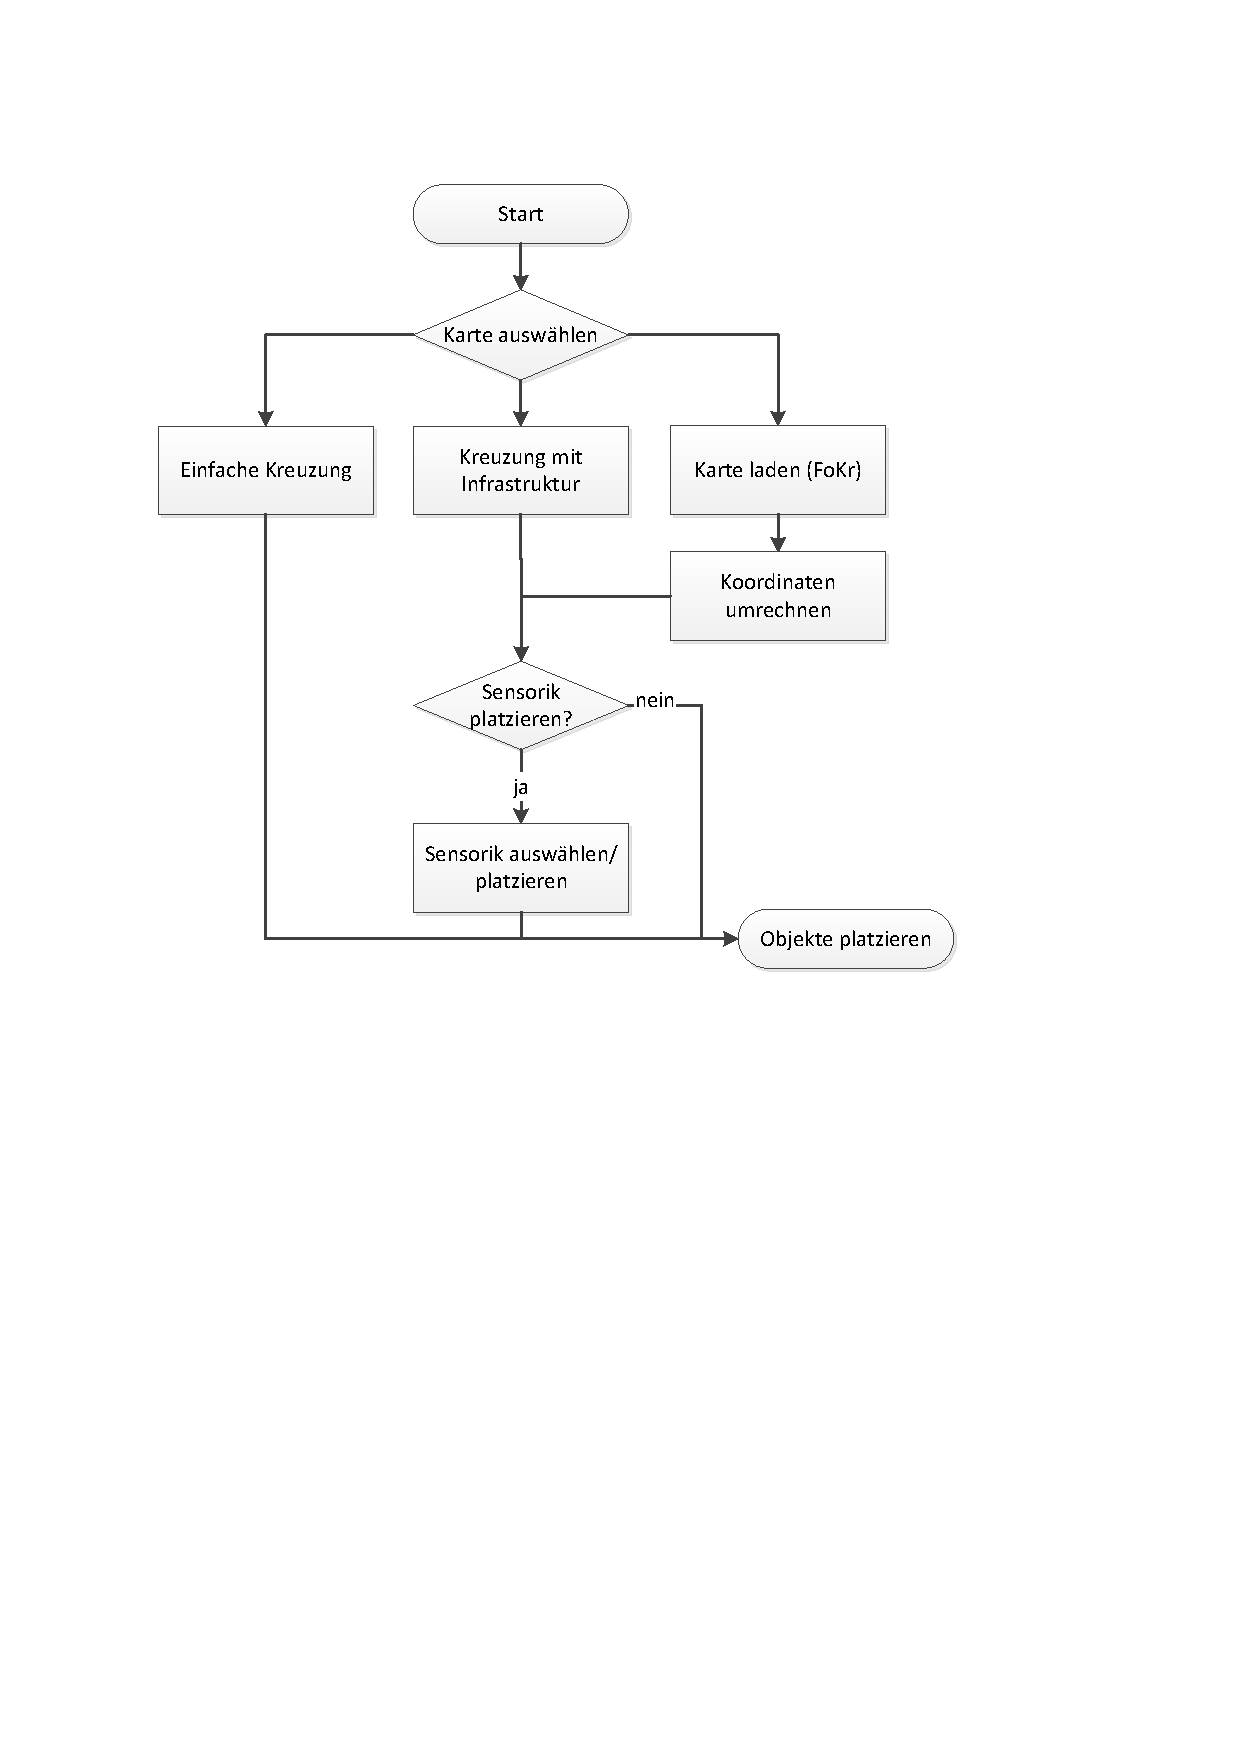
\includegraphics[width=0.8\columnwidth,trim={2.5cm 13.3cm 4.8cm 2.7cm},clip]{pics/Umgebung.pdf}%
\caption{Flussdiagramm der Umgebungserzeugung\label{fig:Umgebung}}%
\end{figure}

\begin{figure}[hbtp]%
\centering
\subfigure[][Kreuzung]{
\includegraphics[width=0.32\textwidth]{pics/Kreuzung.PNG}}\,
\subfigure[][Kreuzung mit Infrastrukturelementen]{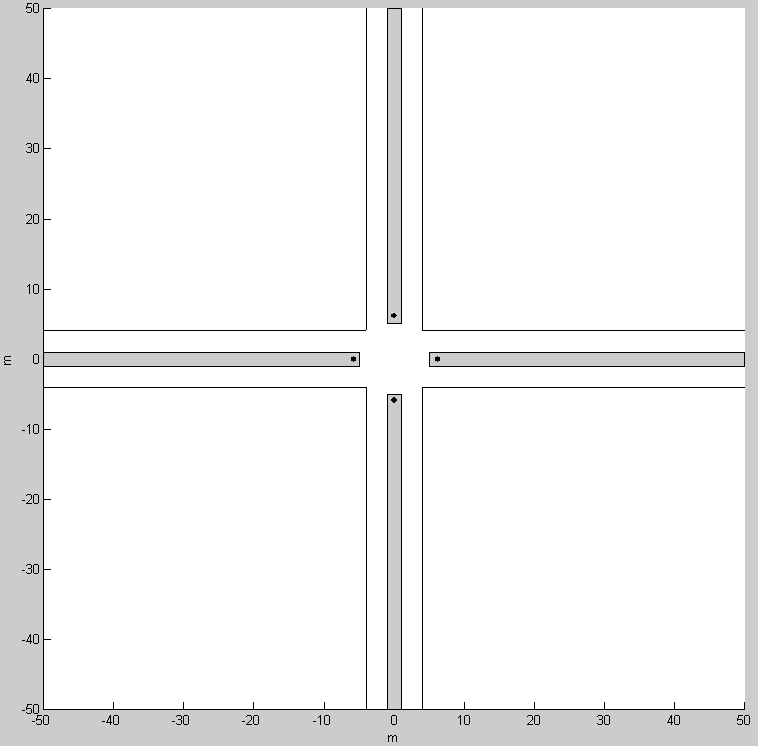
\includegraphics[width=0.32\textwidth]{pics/InfraKreuzung.PNG}}\,%
\subfigure[][Forschungskreuzung]{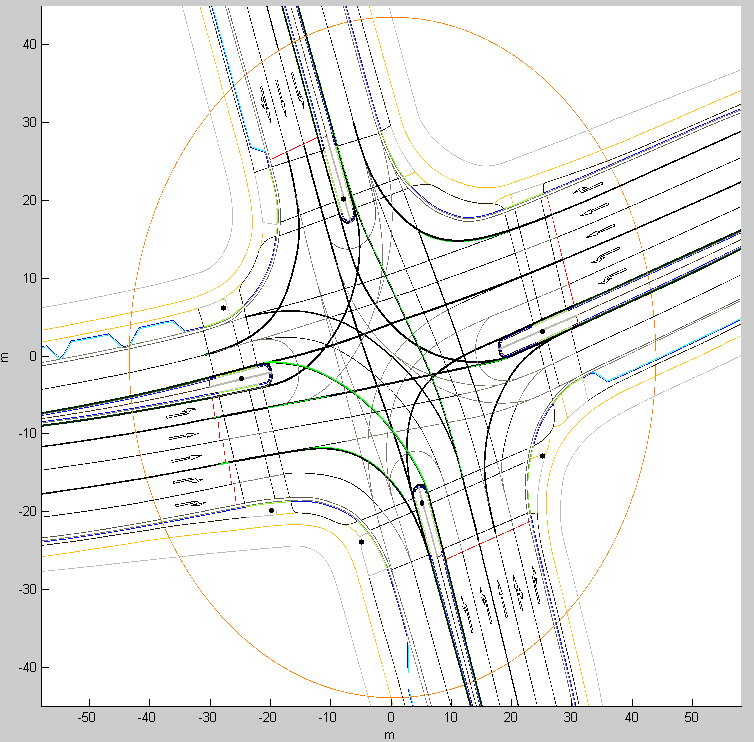
\includegraphics[width=0.32\textwidth]{pics/FoKr.PNG}}%
\caption{Ausw�hlbare Stra�enf�hrungen\label{fig:Kreuzungen}}
\end{figure}

Je nachdem, welche Stra�enf�hrung gew�hlt wird, nimmt das Programm einen anderen Pfad. Bei der einfachen Kreuzung k�nnen nach dem Zeichnen die Objekte platziert werden. Nach dem zeichnen der Kreuzung mit Infrastruktur k�nnen die Infrastrukturelemente mit Sensorik ausgestattet werden. Danach oder wenn dies nicht gew�nscht ist, k�nnen die Objekte platziert werden. Bei der Forschungskreuzung werden zun�chst die TIF- und TFW-Dateien geladen. Mit Hilfe der Daten aus dem World file (TFW) und den Bildpunkten werden die Koordinaten umgerechnet. Anschlie�end k�nnen ebenfalls erst die Sensoren platziert werden oder direkt zur Objektplatzierung weiter gegangen werden.

Neben der Stra�enf�hrung k�nnen die Umwelteinfl�sse Tageszeit und Witterung bestimmt werden (U7, U8). Bei der Tageszeit wird die Variable "`Tag"', bei der Auswahl "`Tag"', auf "`true"' oder, bei der Auswahl "`Nacht"', auf "`false"' gesetzt. Die Auswahl der Witterung geschieht analog zur Tageszeit. F�r die Witterung wird die Variable "`Trocken"' oder "`Nebel"' oder "`Regen"' auf "`true"' und alle anderen auf "`false"' gesetzt. Dies kann vor oder nach der visuellen Erzeugung der Szene ausgew�hlt werden. Wie diese Einfl�sse die Objekterkennung der Sensorik beeinflusst, kann in der Tabelle definiert werden. 

\subsubsection{Objekte}
Die einzelnen Schritte der Objektplatzierung sind in Abbildung\,\ref{fig:Objekte} dargestellt. Solange die Objektanzahl (ObjAnzahl) nicht erreicht worden ist, werden die Schritte ausgef�hrt. Zun�chst wird die Objektposition per Mausklick in der Karte bestimmt (O1). Danach wird der Benutzer aufgefordert einen Objekttypen zu w�hlen (O2). Bei den ersten beiden Stra�enf�hrungen wird im Falle eines Fahrzeugs die Fahrtrichtung der Fahrspur erkannt und der horizontale Ausrichtungswinkel entsprechend gesetzt (O3). Bei Fu�g�ngern und der Forschungskreuzung muss dieser vom Benutzer angegeben werden, da die Extraktion der einzelnen Fahrspuren aus der Bilddatei zu rechenintensiv f�r die Anwendung ist.

\begin{figure}[hbtp]%
\centering
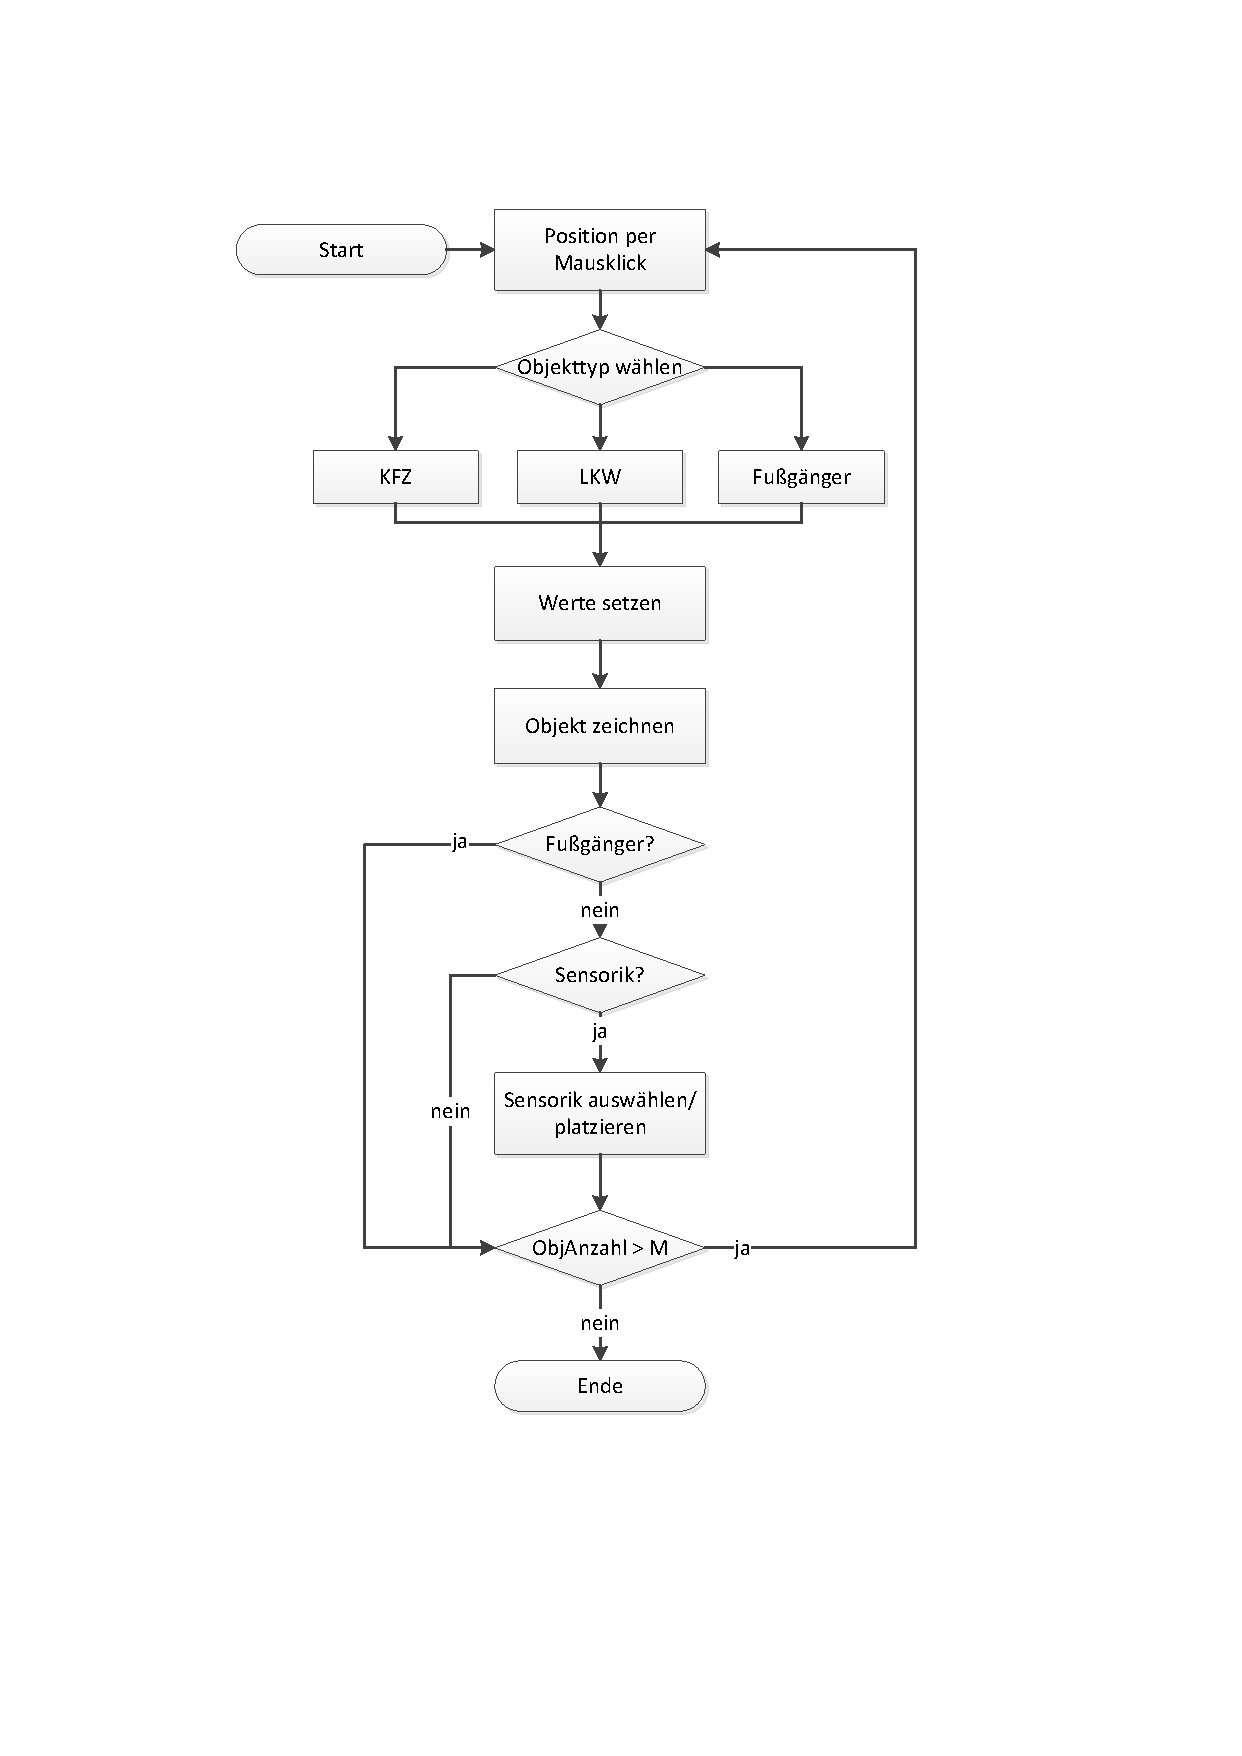
\includegraphics[width=0.7\columnwidth,trim={4cm 5.5cm 5cm 3cm},clip]{pics/Objekte.pdf}%
\caption{Flussdiagramm der Objekterzeugung}%
\label{fig:Objekte}%
\end{figure}

Entsprechend des Objekttyps werden danach Breite $B$, L�nge $L$ und H�he $H$ des Objektes auf die Werte aus Tabelle\,\ref{tab:Grundmasse} gesetzt. Mit der Position, dem Ausrichtungswinkel und den Gr��enangaben werden schlie�lich die Objektecken mit einer homogenen Koordinatentransformation berechnet \cite{F.WahlE.JoernsJ.SchwartzeD.Kubus.}:
\begin{equation}
\begin{bmatrix}
x\\y\\z\\1
\end{bmatrix}
= 
\begin{bmatrix}
	\cos(\alpha) &-\sin(\alpha) &0& x_0\\
  \sin(\alpha) & \cos(\alpha) &0 &y_0\\   
  0 &0& 1& z_0\\
	0 &0 &0 &1
\end{bmatrix}
\cdot
\begin{bmatrix}
\pm \frac{L}{2} \\ \pm\frac{B}{2}\\ H\\1
\end{bmatrix}
\label{eq:Objekt}
\end{equation}

\begin{tabularx}{\textwidth}{lccc}
\caption{Grundma�e von Verkehrsteilnehmern in [\unit{m}] \cite{Wolf.2005}}
\label{tab:Grundmasse}\\\toprule
& \textbf{PKW} & \textbf{LKW} & \textbf{Fu�g�nger}\\\midrule
Breite & 1.75 & 2.55 & 0.55\\
L�nge & 4.7 & 14 & 0.3\\
H�he & 1.7 & 4 & 2\\\bottomrule
\end{tabularx}

Unter Verwendung dieser Eckpunkte wird daraufhin das Objekt als Polygon gezeichnet. Wenn es sich nicht um einen Fu�g�nger handelt, wird der Benutzer aufgefordert, eine Sensoranzahl anzugeben. Ist die Anzahl $>0$, wird das Objekt mit Sensorik ausgestattet. Im Falle eines Fu�g�ngers oder einer Sensoranzahl $=0$ wird dieser Schritt �bersprungen.


\subsubsection{Sensoren}
Der Ablauf f�r die Erzeugung der Sensoren ist in Abbildung\,\ref{fig:Sensor} dargestellt. Als Erstes wird eine Liste mit Sensoren und deren Spezifikationen geladen (siehe Tabelle\,\ref{tab:SensorSpec} im Anhang). Diese Liste wurde aus Datenbl�ttern und anderen Quellen zusammengestellt. Aufgrund der Unterschiede in der Angabe der Spezifikationen sind fehlende Werte durch die typabh�ngige Bestimmung eines Mittelwertes aus den gegebenen Werten anderer Datenbl�tter nachgetragen worden.

\begin{figure}[hbtp]%
\centering
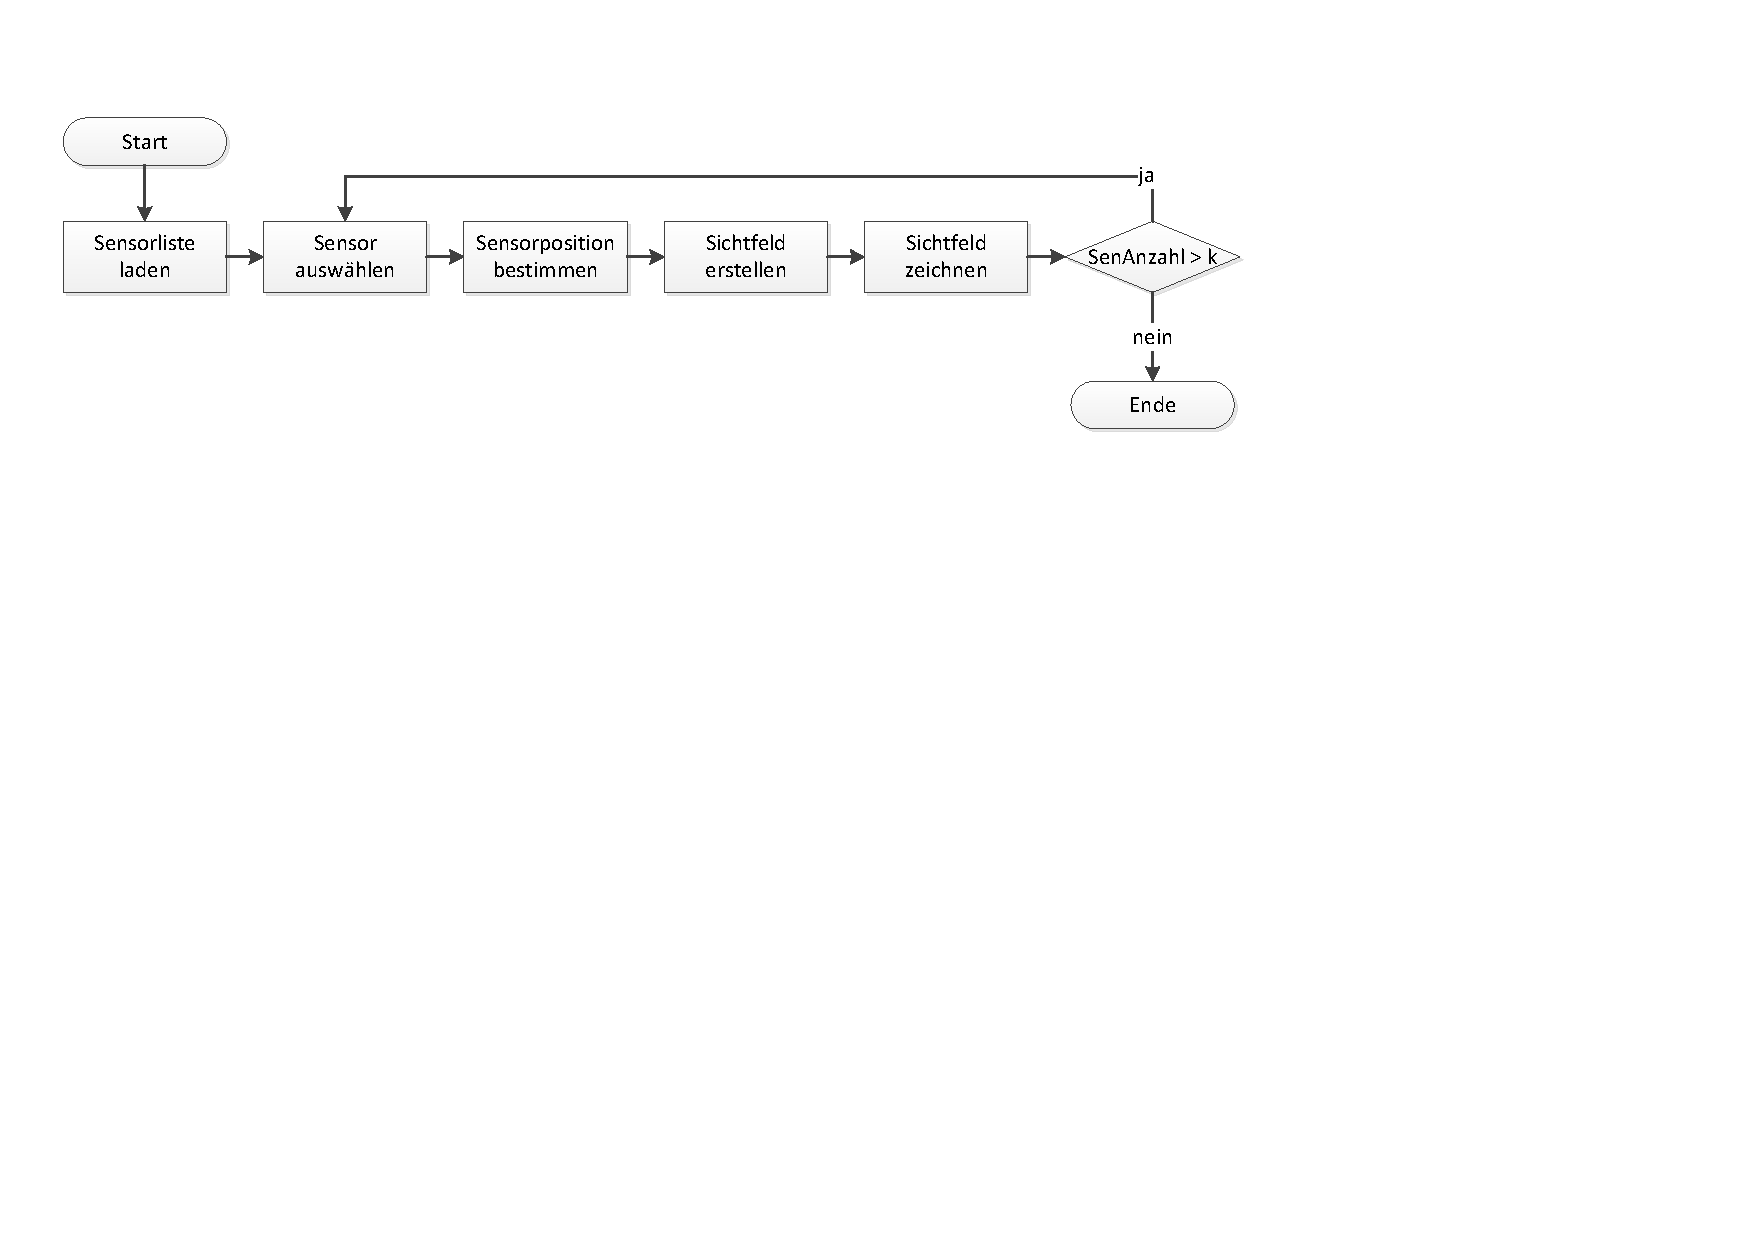
\includegraphics[width=\columnwidth,trim={1cm 13.75cm 8.7cm 1.8cm},clip]{pics/Sensor.pdf}%
\caption{Flussdiagramm der Sensorerzeugung}%
\label{fig:Sensor}%
\end{figure}

Die Sensorliste wird daraufhin dem Benutzer in einem Dialogfenster zur Sensorauswahl angezeigt (S1, S2), siehe Abbildung\,\ref{fig:Sliste}. Nachdem ein Sensor ausgew�hlt worden ist, wird der Benutzer aufgefordert, die Sensorposition und -ausrichtung zu bestimmen (S3, S4), siehe Abbildung\,\ref{fig:ausricht}. Bei der Objektausstattung wird dies innerhalb der Objektkoordinaten durchgef�hrt. 

\begin{figure}[hbtp]%
\centering
\subfigure[][Sensorliste\label{fig:Sliste}]{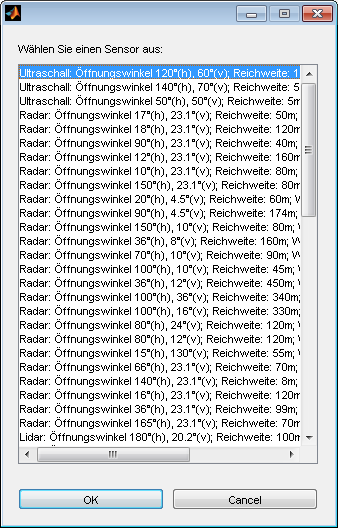
\includegraphics[width=0.3\textwidth]{pics/Sensorliste.png}}\qquad%
\subfigure[][Sensorausrichtung\label{fig:ausricht}]{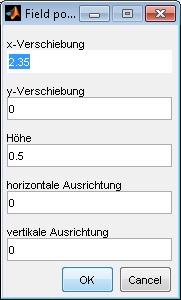
\includegraphics[width=0.25\textwidth]{pics/Sensorausrichtung.png}}%
\caption{Dialogfenster der Sensorausstattung}%
\label{fig:SenAusstattung}%
\end{figure}

Mit Hilfe der Sensorposition, Ausrichtung $\alpha$ und $\beta$, Reichweite $R_{min}$ und $R_{max}$, dem �ffnungswinkel $\phi$ und der Winkelaufl�sung $\Delta \phi$ wird, ebenfalls mit einer homogenen Koordinatentransformation, das Sichtfeld berechnet \cite{F.WahlE.JoernsJ.SchwartzeD.Kubus.}:
\begin{equation}
\begin{bmatrix}
x\\y\\z\\1
\end{bmatrix}
= 
\begin{bmatrix}
	\cos(\alpha) &-\sin(\alpha) &0& x_0\\
  \sin(\alpha) & \cos(\alpha) &0 &y_0\\   
  0 &0& 1& z_0\\
	0 &0 &0 &1
\end{bmatrix}
\cdot
\begin{bmatrix}
 R\sin(\frac{\pi}{2}-\phi)\\ R \cos(\frac{\pi}{2}-\phi)\\ 0\\1
\end{bmatrix}
\label{eq:Sensor}
\end{equation}

F�r den Fall wie in Abbildung\,\ref{fig:Blindspot}, dass der Sensor von oben auf die Szene blickt, wird dessen Sichtfeld f�r die 2D-Projektion verkleinert. Zun�chst wird die minimale Reichweite $R_{min}$ vergr��ert, um den blinden Bereich unterhalb des Sensors zu ber�cksichtigen: 
\begin{equation}
R_{min} = \left|\frac{z_0}{cos\beta}\right|
\label{eq:Rmin}
\end{equation}

\begin{figure}[hbtp]%
\centering
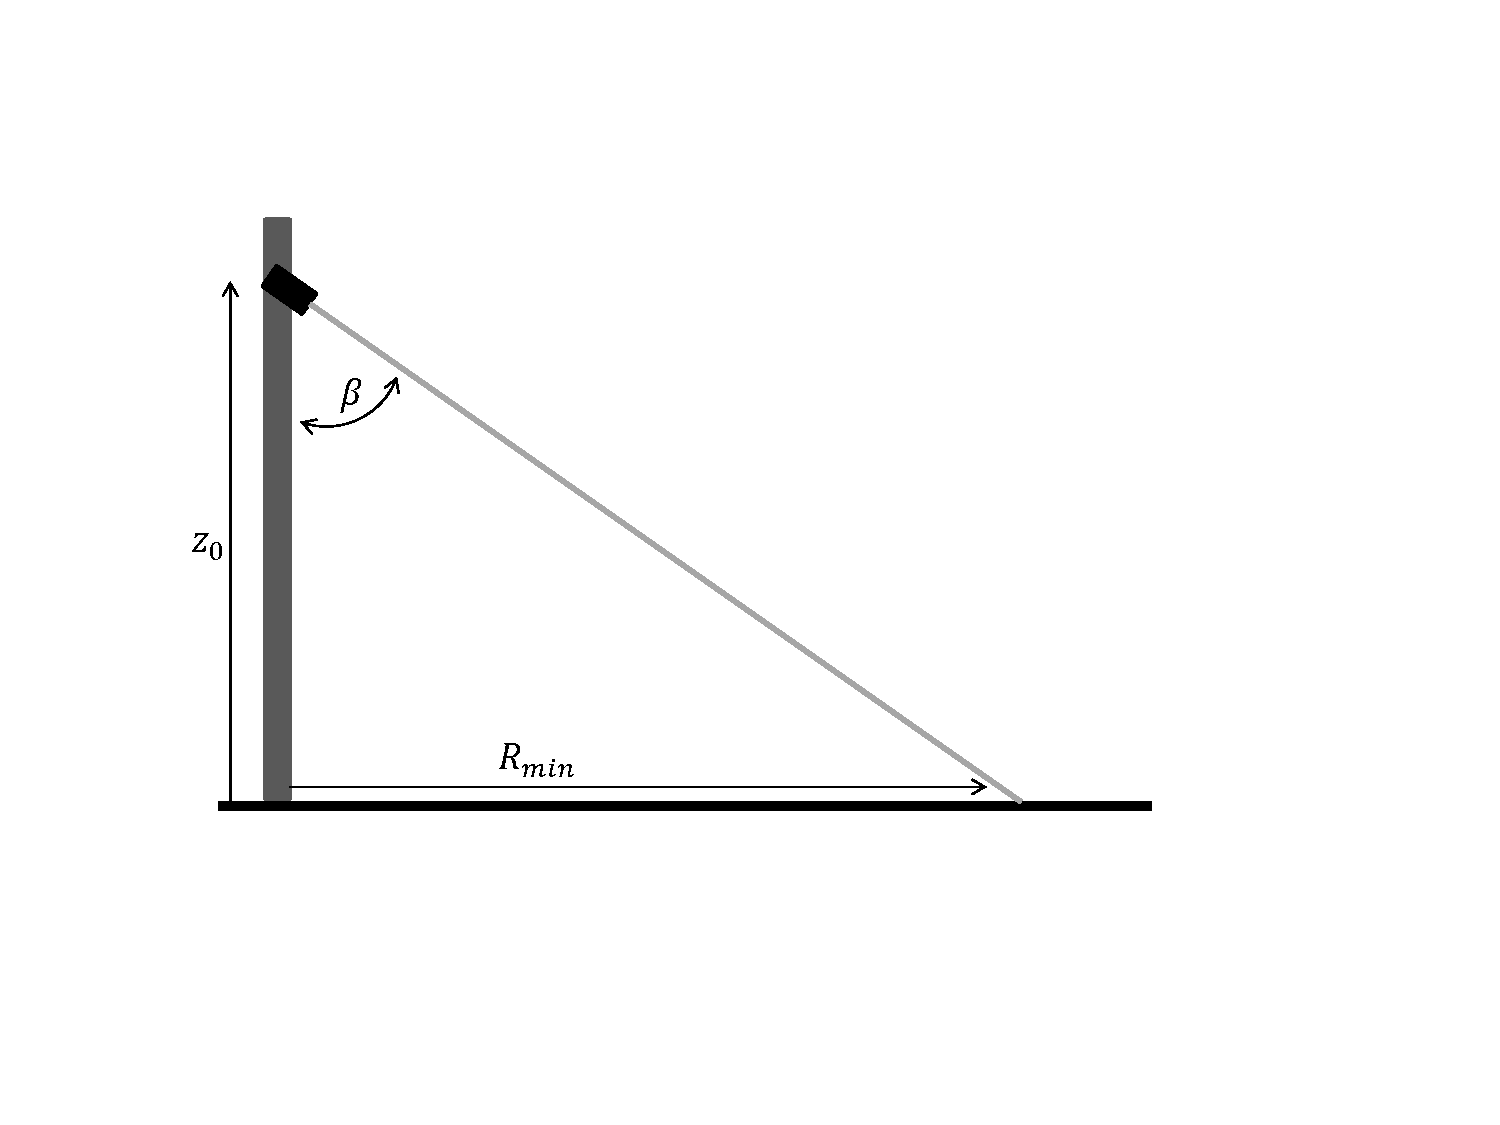
\includegraphics[width=0.65\columnwidth,trim={3cm 5cm 5cm 4cm},clip]{pics/Blindspot.pdf}%
\caption{Ber�cksichtigung des blinden Sensorbereichs}%
\label{fig:Blindspot}%
\end{figure}

Um zus�tzlich zu ber�cksichtigen, dass das Sichtfeld auf den Boden trifft, wird anschlie�end die maximale Reichweite $R_{max}$ um die $R_{min}$ verk�rzt:
\begin{equation}
R_{max} = R_{max} - R_{min}
\label{eq:Rmax}
\end{equation}

Nachdem das Sichtfeld erzeugt worden ist, wird es gezeichnet.

\subsubsection{Auswertung}
Der Ablauf der Auswertung ist in Abbildung\,\ref{fig:Auswertung} dargestellt. Als erstes wird f�r jeden Sensor �berpr�ft, welche Objekte im Sichtfeld liegen (A1). Hierbei wird in jedem Kreisabschnitt mit dem Winkelschritt $d\phi$ �berpr�ft, ob sich Objektpunkte innerhalb des Polygons befinden, siehe Abbildung\,\ref{fig:ObjErkennung}. Danach wird der Objektabstand zum Sensor bestimmt (A4). Nur die Objekte mit dem geringsten Abstand zum Sensor innerhalb des Abschnittes k�nnen als erkannt gesetzt werden. So wird ber�cksichtigt, dass die vorderen Objekte die Sicht auf weiter hinten liegende Objekte behindern. 

\begin{figure}[hbtp]%
\centering
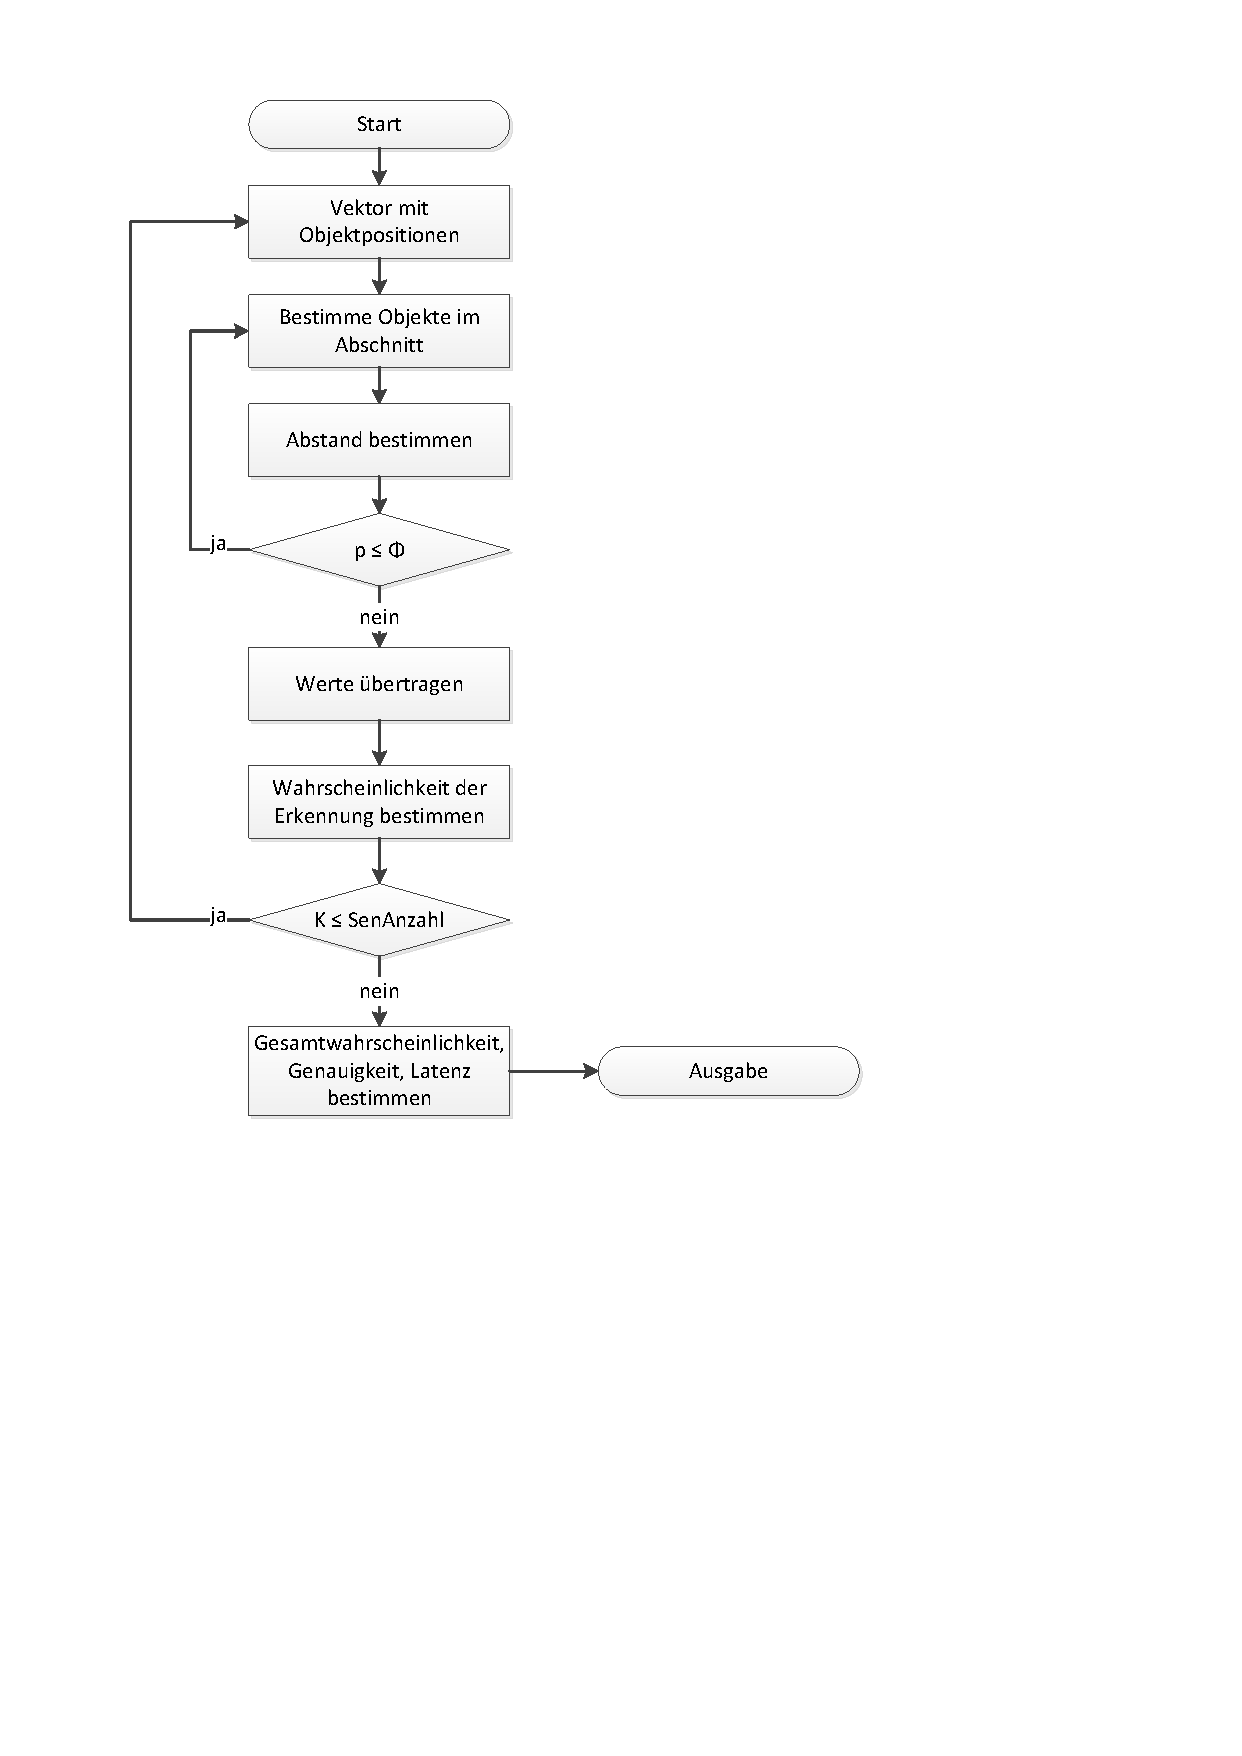
\includegraphics[width=0.8\columnwidth,trim={2.2cm 10.7cm 6.3cm 1.5cm},clip]{pics/Auswertung.pdf}%
\caption{Flussdiagramm der Auswertung}%
\label{fig:Auswertung}%
\end{figure}

\begin{figure}[hbtp]%
\centering
\includegraphics[page=4,width=0.5\textwidth,trim={2cm 7.9cm 10cm 2.5cm},clip]{pics/LidarFoV.pdf}
\caption{Schematische Darstellung der Objekterkennung}%
\label{fig:ObjErkennung}
\end{figure}

Nachdem bestimmt worden ist, welche Objekte der Sensor erfasst, wird die Gesamtwahrscheinlichkeit $p_{Gesamt}$ der Erkennung bestimmt (A3). Hierf�r werden in Abh�ngigkeit vom Sensortyp die Werte aus der Tabelle und der Objektabstand genutzt. Diese Tabelle ist in Abbildung\,\ref{fig:WahrschTab} dargestellt. F�r die Werte in der Tabelle wurden die Erkenntnissen aus Kapitel \ref{chap:Einsatz} herangezogen und zum Teil Annahmen, aufgrund fehlender Daten, getroffen.

\begin{figure}[hbtp]%
\centering
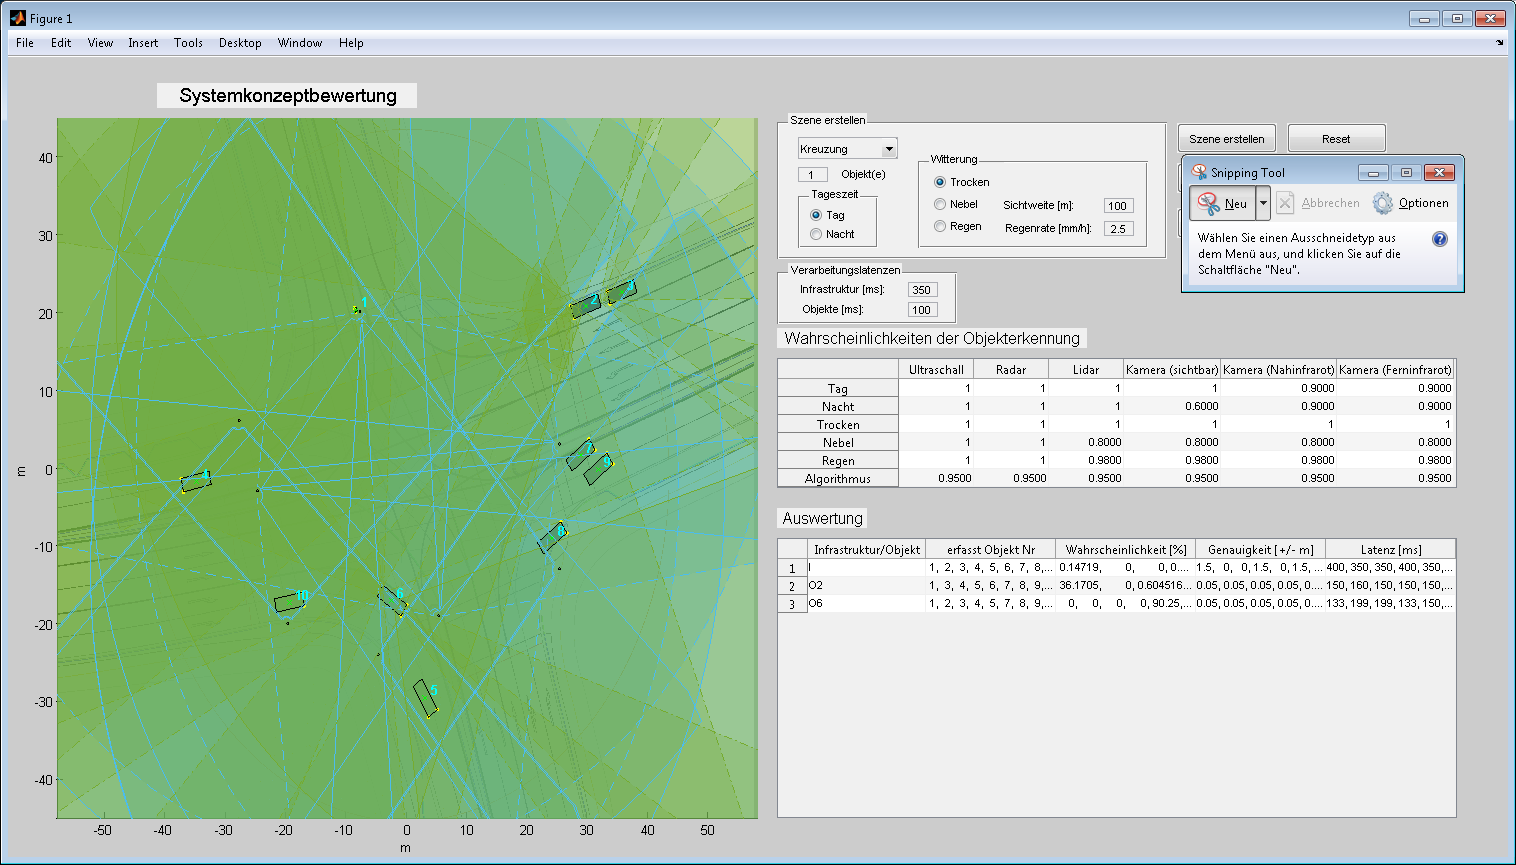
\includegraphics[width=0.9\textwidth,trim={20.5cm 9.95cm 1.5cm 9.5cm},clip]{pics/FoKr-10Obj-bewertet.png}
\caption{Eingabematrix der Wahrscheinlichkeiten der Objekterkennungseinfl�sse}%
\label{fig:WahrschTab}
\end{figure}

Zun�chst wird die Erkennungswahrscheinlichkeit des Objekterkennungsalgorithmus $p_{Algorithmus}$ aus der Tabelle entnommen (A2). Danach wird die Wahrscheinlichkeit $p_{Witterung}$ bei entsprechender Witterung entnommen (S5). Je nach Auswahl der Witterung wird zus�tzlich die Sichtweite bei Nebel oder die Regenrate ber�cksichtigt. Ist Nebel ausgew�hlt worden, wird bei Lidar und Kamera die maximale Reichweite $R_{max}$ verk�rzt und auf die Sichtweite bei Nebel gesetzt. Bei Regen wird bei diesen Sensortypen die Wahrscheinlichkeit $p_{Regen}$ noch zus�tzlich mit der Regenrate $R$ ver�ndert \cite{Goodin.2019}:
\begin{equation}
	p_{Witterung} = p_{Regen} \cdot a R^{c}
	\label{eq:Regen}
\end{equation}

F�r die empirischen Koeffizienten $a$ und $c$ werden die Werte $a=0.01$ und $c=0.6$ aus \cite{Goodin.2019} genutzt. Die American Meteorological Society unterscheidet zwischen vier Regenst�rken: leichter Regen mit $R=$\unitfrac[$\leq$2.5]{mm}{h}, mittlerer Regen mit $R=$\unitfrac[2.5-10]{mm}{h}, starker Regen mit $R=$\unitfrac[10-50]{mm}{h} und schwerer Regen mit $R=$\unitfrac[$\geq$50]{mm}{h} \cite{AmericanMeteorologicalSociety.25.04.2012}.

Anschlie�end wird entweder die Wahrscheinlichkeit f�r die Erkennung bei Tag oder bei Nacht $p_{Tag}$ ausgew�hlt (S6). Nachfolgend wird die Wahrscheinlichkeit $p_{Abstand}$ aufgrund der Objektentfernung bestimmt (A4). Dazu wird eine lineare Funktion in Abh�ngigkeit von der minimalen und maximalen Reichweite bzw. Sichtweite angenommen und mit dem Objektabstand ausgewertet.

%Hierf�r wird die Reichweite geviertelt und �berpr�ft in welchem Quadranten sich das Objekt befindet. Im ersten Quadranten betr�gt die Wahrscheinlichkeit \unit{100}{\%}, im zweiten sind es \unit{75}{\%}, im dritten sind es noch \unit{50}{\%} und im letzten Quadranten betr�gt die Wahrscheinlichkeit nur noch \unit{25}{\%}.

Im Anschluss werden diese Einfl�sse zu der Gesamtwahrscheinlichkeit $p_{Gesamt}$ multipliziert:
\begin{equation}
p_{Gesamt} = p_{Algorithmus}\cdot p_{Witterung}\cdot p_{Tag}\cdot p_{Abstand}
\label{eq:pGesamt}
\end{equation}

Nachdem die Objekterkennung f�r alle Sensoren durchgef�hrt worden ist, werden die Wahrscheinlichkeit, die Genauigkeit und die Latenz, mit der ein Objekt erkannt wird, bestimmt (A8). Daf�r wird zun�chst der jeweilige Wert vom Sensor �bertragen. Wenn ein Wert eines anderen Sensors der Infrastruktur oder Objektes vorliegt, wird bei der Latenz der kleinere von beiden Werten genutzt. Von diesem Sensor wird au�erdem die Genauigkeit �bertragen. Bei der Wahrscheinlichkeit wird der jeweils gr��ere Wert genommen.

Zuletzt werden diese Werte in einer Ausgabematrix auf der Benutzeroberfl�che ausgegeben. Diese ist in Abbildung\,\ref{fig:AuswertungTab} dargestellt.
\begin{figure}[hbtp]%
\centering
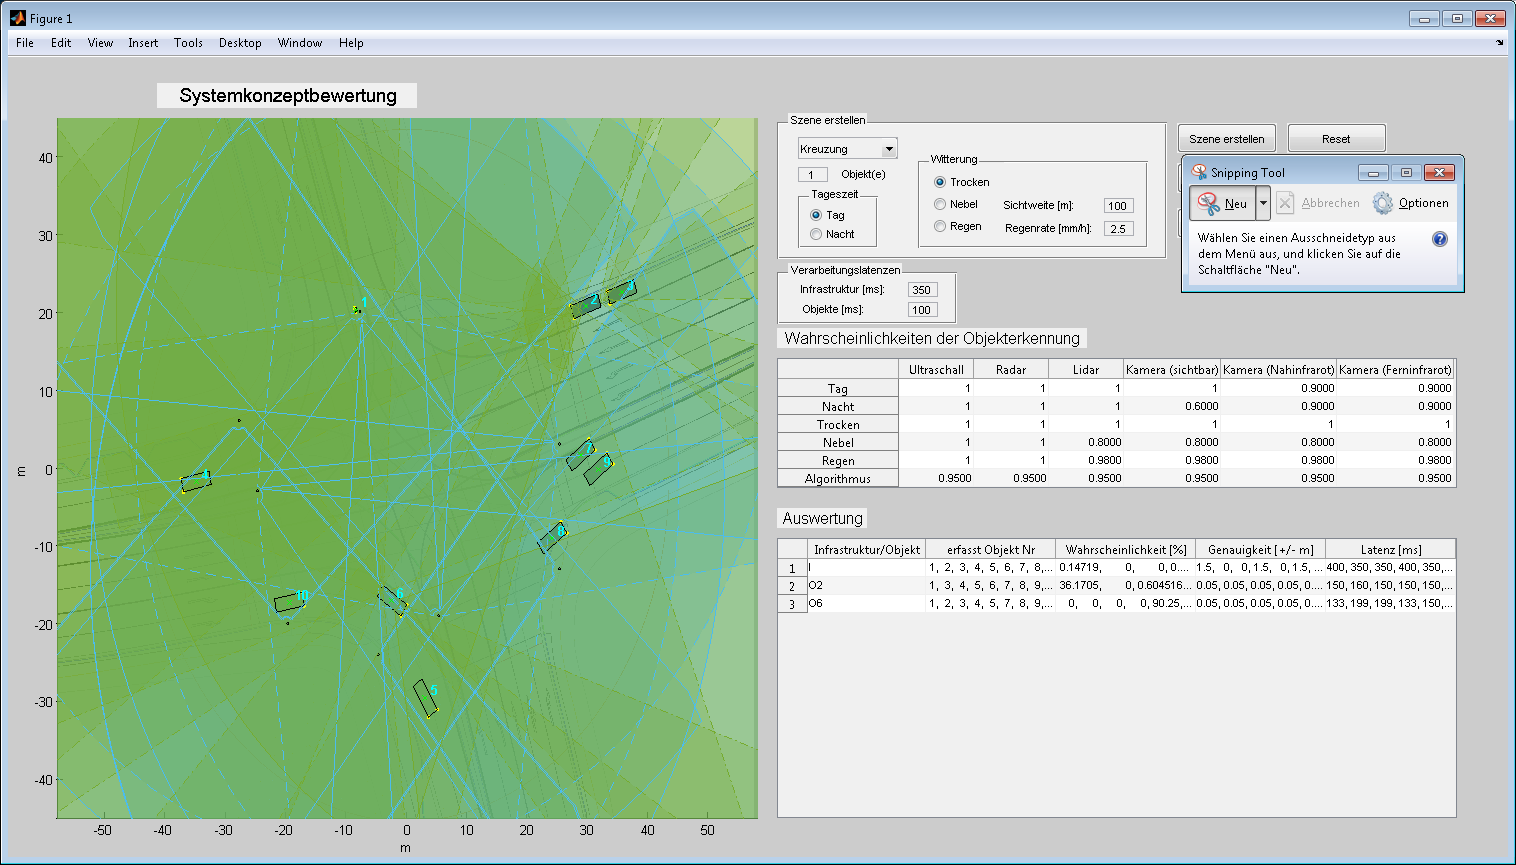
\includegraphics[width=0.9\textwidth,trim={20.5cm 1.1cm 1.5cm 14.2cm},clip]{pics/FoKr-10Obj-bewertet.png}
\caption{Ausgabematrix der Auswertung}%
\label{fig:AuswertungTab}
\end{figure}

\section{Studie zur Anwendung des Tools}
\label{chap:Anwendung}
F�r die Bewertung des Simulations-Tools werden in diesem Kapitel vier verschiedene Szenen ausgewertet. Die ersten beiden Beispielen thematisieren die Einfl�sse auf die Objekterkennung. Die letzten zwei Szenen umfassen reale Anwendungsbeispiele. F�r die Auswertung von mehreren Zeitschritten wurde ein Mechanismus implementiert, der die Szenendaten automatisch l�dt und auswertet. Eine Evaluation der Ergebnisse schlie�t das Kapitel ab.

%\subsection{Verifikation}
%\label{sec:Verifikation}
\subsection{Einfluss des Objektabstandes}
\label{sec:Abstand}
Diese Szene �berpr�ft den Einfluss des Objektabstandes auf die Objekterkennung, siehe Abbildung\,\ref{fig:Probe}. Sie besteht aus einer Kreuzung und zwei Fahrzeugen, die sich mit jeweils \unitfrac[50]{km}{h} aufeinander zu bewegen. Objekt\,1 (in der unteren Bildh�lfte) ist mit einem einzelnen Sensor vom Typ Radar ausgestattet, dessen Spezifikationen der Tabelle\,\ref{tab:ProbeKonfig} zu entnehmen sind.

\begin{figure}[!hbtp]%
\centering
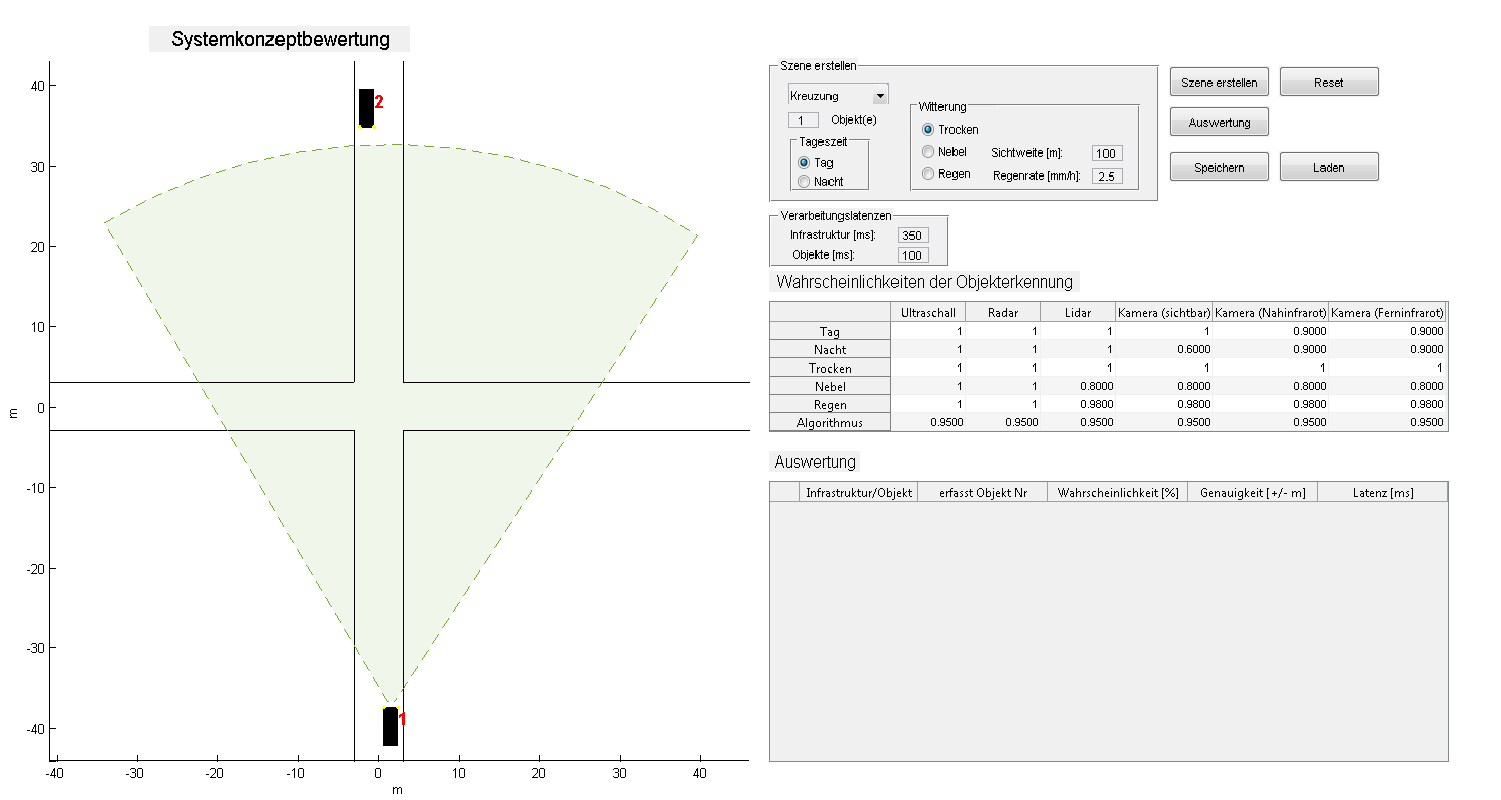
\includegraphics[width=0.77\textwidth,trim={0.2cm 0.1cm 19.9cm 2.0cm},clip]{pics/Probeszene.PNG}
\caption{Ausgangssituation f�r die Darstellung des Einfluss des Objektabstandes\label{fig:Probe}}
\end{figure}

\begin{tabularx}{\textwidth}{lccccc}%
\caption{Sensorkonfiguration von Objekt\,1}
\label{tab:ProbeKonfig}\\\toprule
\textbf{Anz}&\textbf{Typ}	&$\boldsymbol{\phi_H$/$\phi_V}$ \textbf{[�]}	& $\boldsymbol{R_{min}$/$R_{max}}$ \textbf{[m]}&\textbf{Tol [$\pm$m]	}& $\boldsymbol{T_{Mess}}$ \textbf{[ms]}	\\ \midrule
1&Radar&	66/23.1&	0.82/70&	0.36&	60	\\\bottomrule
\end{tabularx}

Abbildung\,\ref{fig:ProbeWahr} zeigt den zeitlichen Verlauf der Erkennungswahrscheinlichkeit und des Objektabstandes. Die Szene wurde alle \unit[160]{ms} ausgewertet, was der Summe aus der Messlatenz $T_{Mess}$ des Sensors und der angegebenen Verarbeitungslatenz des Fahrzeugs von \unit[100]{ms} entspricht. Zu den ersten beiden Zeitpunkten befindet sich das Objekt\,2 noch au�erhalb der Sensorreichweite und wird somit nicht erkannt. Mit abnehmender Entfernung nimmt die Wahrscheinlichkeit, dass es erkannt wird, linear zu. Dies entspricht dem implementierten Ansatz zur Forderung einer Abh�ngigkeit der Erkennungswahrscheinlichkeit vom Objektabstand.

\begin{figure}[hbtp]%
\centering
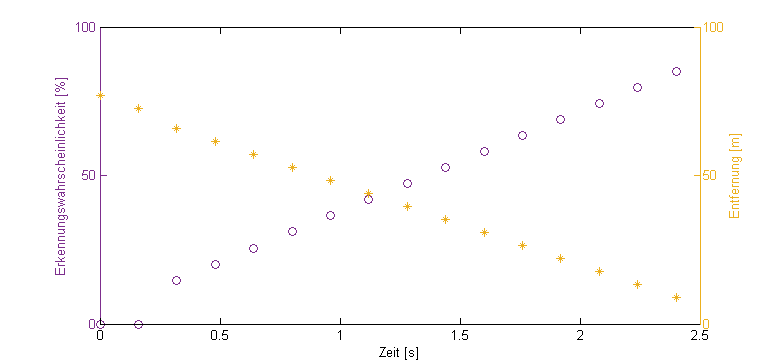
\includegraphics[width=\columnwidth,trim={0.9cm 0.1cm 0.5cm 0.5cm},clip]{pics/fig_Probe_Wahrscheinlichkeit_Entfernung.png}%
\caption{Zeitverlauf der Erkennungswahrscheinlichkeit und des Objektabstandes\label{fig:ProbeWahr}}%%
\end{figure}

\newpage
Aufgrund der angegebenen Wahrscheinlichkeit des Objekterkennungsalgorithmus von $p_{Algorithmus}=$\unit[95]{\%} und der Tatsache, dass das Objekt\,2 an Objekt\,1 vorbei f�hrt, wird eine Erkennungswahrscheinlichkeit von $p_{Gesamt}=$\unit[100]{\%} nicht erreicht. Nach \unit[2.5]{s} hat Objekt\,2 schlie�lich das Sensorsichtfeld wieder verlassen und wird nicht mehr erfasst. 


%\newpage

\subsection{Umwelteinfl�sse}
\label{sec:Umwelteinfluss}
Abbildung\,\ref{fig:Einfluss} zeigt ein Objekt im Sensorsichtfeld einer Kamera, die an einem Infrastrukturelement montiert ist. Die Sensorspezifikationen sind in Tabelle\,\ref{tab:EinflussKonfig} aufgef�hrt.  Mit dieser Szene sollen die Umwelteinfl�sse auf die Objekterkennung untersucht werden. Aufgrund ihrer hohen Empfindlichkeit auf Umwelteinfl�sse wurde f�r dieses Beispiel eine Kamera, die nur das sichtbare Spektrum erfasst, ausgew�hlt.

\begin{figure}[!hbtp]%
\centering
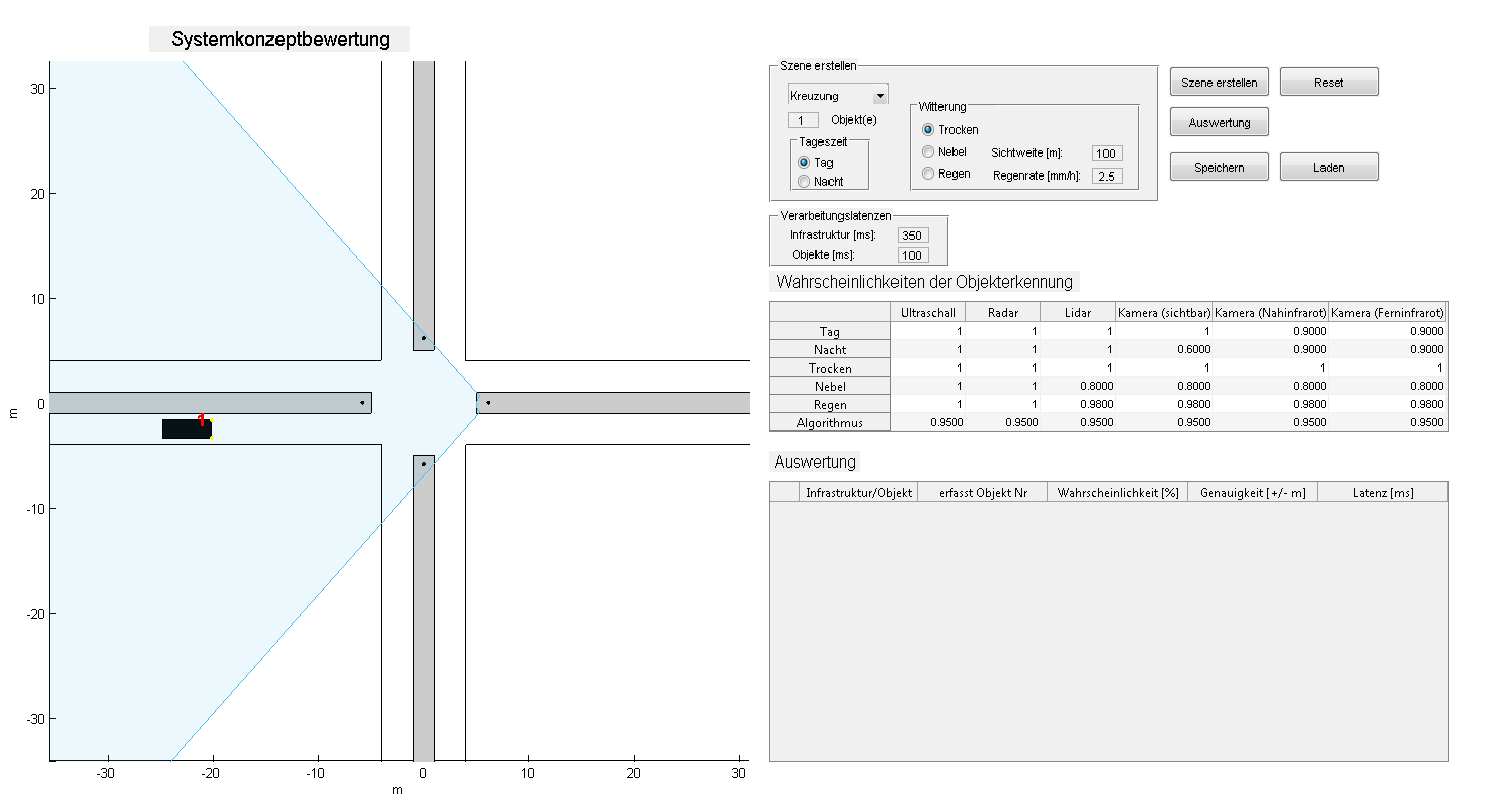
\includegraphics[width=0.77\textwidth,trim={0.2cm 0.1cm 19.9cm 1.7cm},clip]{pics/Einfluss.PNG}
\caption{Infrastruktur erfasst mit einer Kamera ein Objekt \label{fig:Einfluss}}
\end{figure}
 %\newpage
\begin{tabularx}{\textwidth}{lp{1.7cm}cccc}%
\caption{Sensorkonfiguration der Infrastruktur}
\label{tab:EinflussKonfig}\\\toprule
\textbf{Anz}&\textbf{Typ}	&$\boldsymbol{\phi_H$/$\phi_V}$ \textbf{[�]}	& $\boldsymbol{R_{min}$/$R_{max}}$ \textbf{[m]}&\textbf{Tol [$\pm$m]	}& $\boldsymbol{T_{Mess}}$ \textbf{[ms]}	\\ \midrule
1&Kamera (sichtbar)	&97/74	&1/77.5	&0.25	&50	\\\bottomrule
\end{tabularx}

Der Abstand zwischen Objekt und Kamera betr�gt \unit[28.6]{m}. Er bleibt konstant, da nur ein Zeitpunkt betrachtet wird, um den Einfluss der durch die Abstands�nderung auszuschlie�en. F�r die Bewertung des Regeneinflusses wurde die Szene mit verschiedenen Regenraten ausgewertet. Die �berpr�fung des Einflusses von Nebel wurde durchgef�hrt, indem die Szene mit unterschiedlichen Sichtweiten ausgewertet wurde. Beides wurde mit den Tageszeiteinstellungen "`Tag"' und "`Nacht"' durchgef�hrt.
%\newpage

Die Ergebnisse f�r den Einfluss von Regen bei Tag und Nacht sind in Abbildung\,\ref{fig:EinflussRegen} dargestellt. Die Punkte bei einer Regenrate von \unitfrac[0]{mm}{h} entsprechen dem Ergebnis bei der Witterungsauswahl "`Trocken"'. Aufgrund des Objektabstandes wird ohne Regen eine Erkennungswahrscheinlichkeit von etwa \unit[65]{\%} am Tage und von \unit[39]{\%} bei Nacht erreicht. Es ist zu erkennen, dass Regen die Objekterkennung kaum beeinflusst. Der Einfluss liegt unter \unit[10]{\%} bei Regenraten von bis zu \unitfrac[40]{mm}{h}, was starkem Regenfall entspricht \cite{AmericanMeteorologicalSociety.25.04.2012}. Dieses Ergebnis ist zu erwarten, da  in \cite{Goodin.2019} der ermittelte Einfluss von Regen gering ausf�llt.

\begin{figure}[hbtp]%
\centering
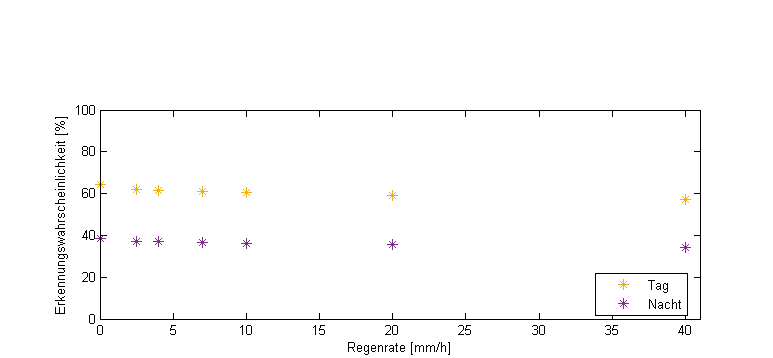
\includegraphics[width=\textwidth,trim={1cm 0.05cm 1.8cm 2.7cm},clip]{pics/Regen.PNG}%
\caption[Einfluss von Regen auf die Erkennungswahrscheinlichkeiten]{Einfluss von Regen auf die Erkennungswahrscheinlichkeiten einer Kamera im sichtbaren Spektrum bei Tag und Nacht\label{fig:EinflussRegen}}
\end{figure}

Abbildung\,\ref{fig:EinflussNebel} zeigt die Ergebnisse f�r den Einfluss von Nebel bei Tag und Nacht. Die Objekterkennung bei Nebel wird deutlich st�rker beeinflusst als bei Regen. Dies ist zum Einen auf die Reduktion der Sichtweite und zum Anderen auf den kleineren Wert der Einflusswahrscheinlichkeit zur�ckzuf�hren. W�hrend am Tage bei Regen die Erkennungswahrscheinlichkeit nicht unter \unit[55]{\%} f�llt, ist dies bei Nebel schon f�r Sichtweiten unter \unit[120]{m} der Fall. Die Tageszeit f�hrt in beiden F�llen lediglich zu einer negativen Verschiebung entlang der y-Achse.

Nebel mit Sichtweiten, welche die Reichweite dieses Sensors von $R_{max}=$\unit[77.5]{m} �bersteigen, reduzieren nicht die Reichweite. Ab diesem Wert wird ausschlie�lich die in der Tabelle eingetragene Einflusswahrscheinlichkeit f�r Nebel ber�cksichtigt. Aus diesem Grund ist die Erkennungswahrscheinlichkeit ab diesem Wert nahezu konstant.

\begin{figure}[hbtp]%
\centering
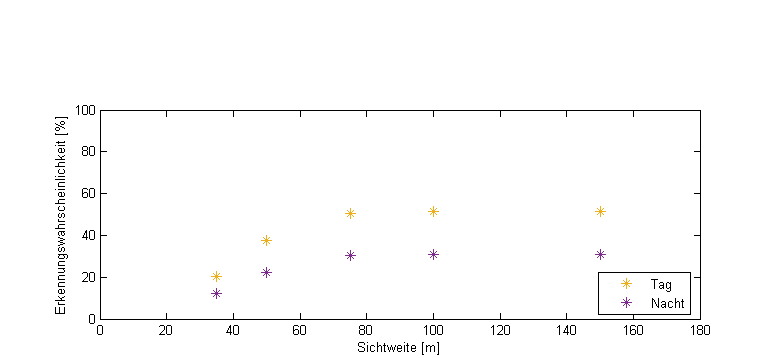
\includegraphics[width=\textwidth,trim={1cm 0.05cm 1.5cm 2.7cm},clip]{pics/Nebel.PNG}
\caption[Einfluss von Nebel auf die Erkennungswahrscheinlichkeiten]{Einfluss von Nebel auf die Erkennungswahrscheinlichkeiten einer Kamera im sichtbaren Spektrum bei Tag und Nacht\label{fig:EinflussNebel}}
\end{figure}

%\newpage
%\subsection{Evaluation}
%\label{sec:Evaluation}
\subsection{Vergleich von zwei Sensorkonfigurationen}
\label{sec:Vergleich}
Ein Anwendungsfall ist der Vergleich von verschiedenen Sensorkonfigurationen. Dies wurde im Rahmen dieser Arbeit beispielhaft mit den Forschungsfahrzeugen \acs{TIAMO} der \acs{TU BS} und dem \acs{FASCarE} des \acs{DLR} durchgef�hrt, siehe Abbildung \ref{fig:Fahrzeugsensoren}. Die Sensorkonfigurationen der beiden Fahrzeuge sind in Tabelle\,\ref{tab:VglKonfig} aufgef�hrt. Der Einbauort der Sensoren ist mit F (Front) und H (Heck) gekennzeichnet. 

%\newpage
\begin{tabularx}{\textwidth}{lcp{1.7cm}cccc}%
\caption{Sensorkonfigurationen des \acs{FASCarE} (\acs{DLR}) und des \acs{TIAMO} (\acs{TU BS})}
\label{tab:VglKonfig}\\\toprule
\multicolumn{7}{c}{\textbf{\acs{FASCarE}}}\\\midrule
\textbf{Anz}&\textbf{Ort}&\textbf{Typ}	&$\boldsymbol{\phi_H$/$\phi_V}$ \textbf{[�]}	& $\boldsymbol{R_{min}$/$R_{max}}$ \textbf{[m]}&\textbf{Tol [$\pm$m]	}& $\boldsymbol{T_{Mess}}$ \textbf{[ms]}	\\ \midrule
5&F&Lidar&	110/3.2&	0.3/200		&0.05	&80	\\
2&F&Radar	&66/23.1	&0.82/70		&0.36	&60	\\
1&F&Radar	&12/23.1	&0.36/160		&0.12	&60	\\
1&F&Kamera (sichtbar)	&50/28	&1/120	&0.25	&33	\\
1&H&Lidar&	110/3.2&	0.3/200		&0.05	&80	\\	
2&H&Radar	&140/23.1	&0.82/8		&0.36	&60	\\	
1&H&Radar	&16/23.1	&0.82/120		&0.36	&60	\\\midrule

\multicolumn{7}{c}{\textbf{\acs{TIAMO}}}\\\midrule
\textbf{Anz}&\textbf{Ort}&\textbf{Typ}	&$\boldsymbol{\phi_H$/$\phi_V}$ \textbf{[�]}	& $\boldsymbol{R_{min}$/$R_{max}}$ \textbf{[m]}&\textbf{Tol [$\pm$m]	}& $\boldsymbol{T_{Mess}}$ \textbf{[ms]}	\\ \midrule
2&F&Lidar	&110/3.2&	0.3/200	&	0.05&	80	\\
1&F&Radar&	12/23.1&	0.36/160	&	0.12&	60	\\
1&F&Kamera (sichtbar)&	50/28	&1/120&	0.25	&33	\\
1&H&Lidar	&190/20.2	&0/80	&	0.025	&13	\\
2&H&Lidar	&110/3.2&	0.3/200	&	0.05&	80	\\
2&H&Radar	&165/23.1	&0.75/70	&1.50	&50	\\\bottomrule
\end{tabularx} 

Das \acs{FASCarE} ist mit 13 Sensoren ausgestattet und am \acs{TIAMO} sind neun Sensoren verbaut. In der Front ist das \acs{FASCarE} mit drei Radaren, f�nf Lidaren und einer Kamera teils redundant und teils komplement�r ausgestattet. Beim \acs{TIAMO} werden ein Radar, zwei Lidare und eine Kamera redundant und komplement�r in der Front verwendet. Am Heck hingegen sind beim \acs{TIAMO} f�nf Sensoren verbaut, w�hrend das \acs{FASCarE} am Heck mit vier Sensoren ausgestattet ist.% wovon zwei eine Reichweite von \unit[8]{m} aufweisen.

F�r die Bewertung der beiden Fahrzeugkonfigurationen wurden diese in die gleiche Szene gesetzt, die in den Abbildungen\,\ref{fig:VglFASCarE} und \ref{fig:VglTIAMO} f�r beide Fahrzeuge dargestellt ist. Die Szene ist eine Momentaufnahme mit insgesamt sieben Fahrzeugen, die auf eine Kreuzung zufahren. Das Objekt\,1 wurde jeweils mit der Fahrzeugkonfiguration des \acs{FASCarE} und des \acs{TIAMO} ausgesattet. In beiden F�llen ist zu erkennen, dass die Sichtfelder beider Fahrzeuge nahezu die gesamte Umgebung abdecken. Des Weiteren verdeutlichen diese Abbildungen noch einmal die Redundanzen der Sichtfelder.

\begin{figure}[hbtp]%
\centering
\subfigure[][\acs{FASCarE}\label{fig:VglFASCarE}]{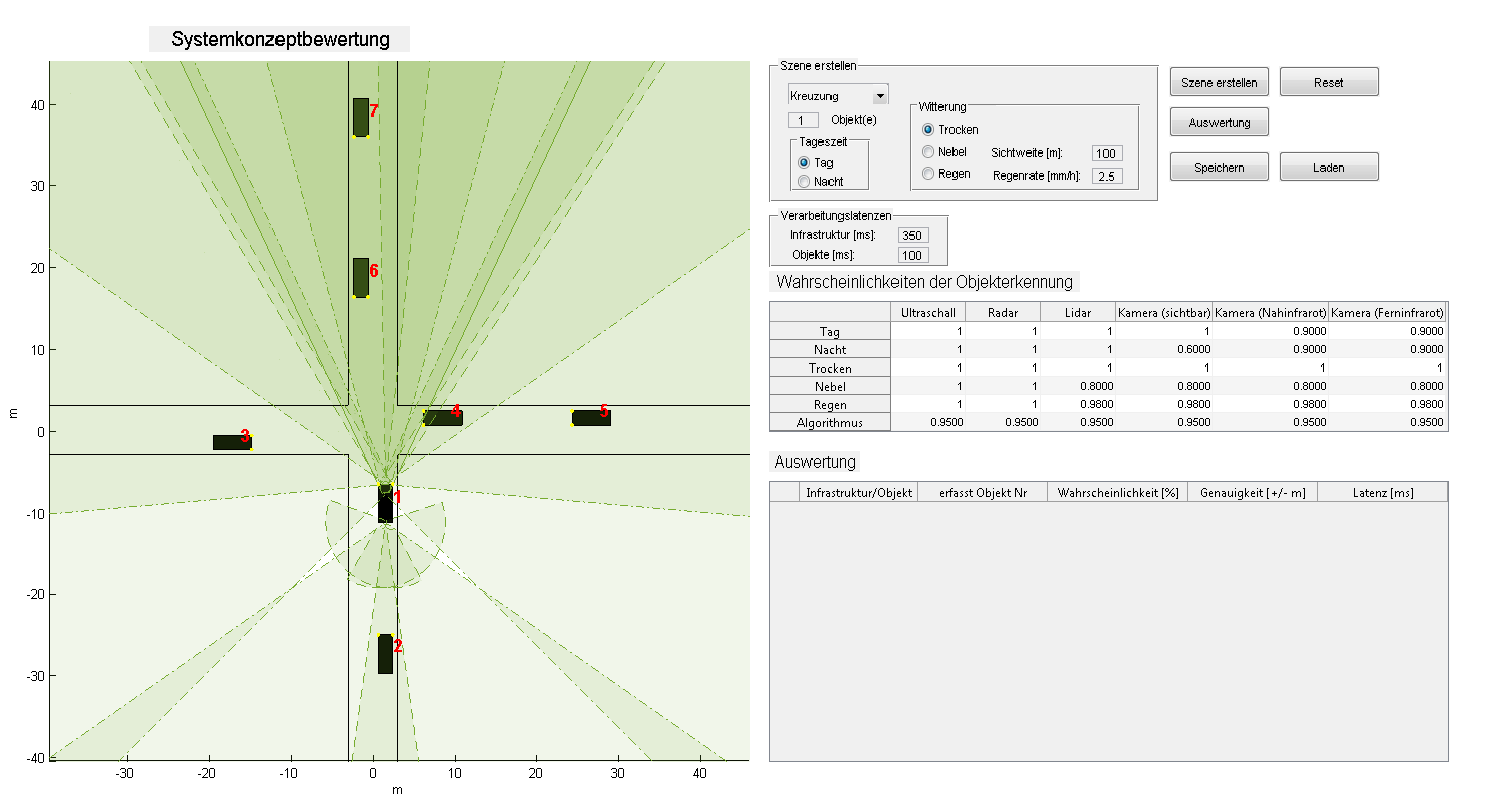
\includegraphics[width=0.49\textwidth,trim={0.2cm 0.1cm 19.9cm 2.0cm},clip]{pics/Vergleich_FASCarE.PNG}}\,
\subfigure[][\acs{TIAMO}\label{fig:VglTIAMO}]{\includegraphics[width=0.49\textwidth,trim={0.2cm 0.1cm 19.9cm 2.0cm},clip]{pics/Vergleich_TIAMO.PNG}}%
\caption{Szene zum Vergleich der Sensorkonfiguration vom \acs{FASCarE} und \acs{TIAMO}\label{fig:VglSzene}}
\end{figure}

Tabelle\,\ref{tab:VglLatGen} f�hrt die erfassten Objekte und die Genauigkeit und Latenz der Messung in dem untersuchten Zeitpunkt auf. Beide Fahrzeuge erfassen alle sechs Objekte, jedoch mit unterschiedlichen Genauigkeiten und Latenzen. Das Objekt\,2 wird vom \acs{TIAMO} \unit[47]{ms} fr�her und mit einer h�heren Genauigkeit erfasst als vom \acs{FASCarE}, da ein Lidar mit h�herer Genauigkeit und geringerer Latenz beim \acs{TIAMO} verbaut ist. Die Objekte\,3 und 5 werden ebenfalls vom \acs{TIAMO} fr�her erfasst, jedoch mit einer Genauigkeit von \unit[$\pm$1.5]{m}. \unit[30]{ms} sp�ter, wenn die Daten aller Sensoren vorliegen, w�re die Genauigkeit ebenfalls bei \unit[$\pm$0.05]{m}. Das Objekt\,4 wird von beiden mit dem gleichen Lidar und die Objekte 6 und 7 werden von beiden mit der gleichen Kamera erfasst, weswegen es keine Unterschiede bez�glich der Latenz und Genauigkeit gibt.
\newpage

\begin{tabularx}{\textwidth}{lcccccc}%
%\centering
\caption[Genauigkeiten und Latenzen der zwei Sensorkonfigurationen]{Genauigkeiten und Latenzen der Sensorkonfigurationen des \acs{FASCarE} (\acs{DLR}) und des \acs{TIAMO} (\acs{TU BS})}
\label{tab:VglLatGen}\\\toprule%\hline
 \multicolumn{7}{c}{\textbf{\acs{FASCarE}}}\\\midrule%\hline
\textbf{erfasst Objekt} & 2& 3& 4& 5& 6& 7 \\ 
\textbf{Genauigkeit [\unit{$\pm$}{m}}] & 0.36 &0.05& 0.05 &0.05& 0.25& 0.25 \\
\textbf{Latenz [\unit{ms}}] & 160 & 180 & 180& 180 &133 &133\\\midrule %\hline
 \multicolumn{7}{c}{\textbf{\acs{TIAMO}}}\\\midrule
\textbf{erfasst Objekt} & 2& 3& 4& 5& 6& 7\\
\textbf{Genauigkeit [\unit{$\pm$}{m}}] & 0.025 &  1.5 & 0.05  & 1.5 & 0.25 & 0.25\\
\textbf{Latenz [\unit{ms}}]& 	113 & 150 & 180 & 150 & 133 & 133\\\bottomrule
\end{tabularx} 

%\newpage
Wird hingegen die Erkennungswahrscheinlichkeit beider Fahrzeuge in Abbildung\,\ref{fig:VglWahr} verglichen, f�llt nur bei Nebel ein deutlicher Unterschied auf (Sterne und Kreise in Rot). Aufgrund der h�heren Reichweite des Heckradars beim \acs{FASCarE} erfasst dieses das Objekt\,2 mit einer Wahrscheinlichkeit von \unit[84]{\%} bei Nebel mit einer Sichtweite von \unit[100]{m}. Die Erkennungswahrscheinlichkeit des \acs{TIAMO} f�r das Objekt\,2 betr�gt hingegen \unit[76]{\%}. Die Objekte\,3 und 5 werden vom \acs{TIAMO} durch die Heckradare bei Nebel mit einer h�heren Wahrscheinlichkeit erfasst als von den Frontlidaren des \acs{FASCarE}. Diese betragen \unit[69]{\%} und \unit[60]{\%} beim \acs{TIAMO} und \unit[62]{\%} und \unit[57]{\%} beim \acs{FASCarE}. Objekt\,6 wird mit \unit[64]{\%} hingegen vom \acs{FASCarE} aufgrund der Frontradare besser erfasst als vom \acs{TIAMO} mit \unit[58]{\%}. Der vollst�ndigkeithalber wurde au�erdem eine Auswertung bei Nacht durchgef�hrt. Da Radar und Lidar von der Tageszeit unabh�ngig sind ist diese Auswertung in Abbildung\,\ref{fig:VglWahrNacht} im Anhang zu finden.

\begin{figure}[!hbtp]%
\centering
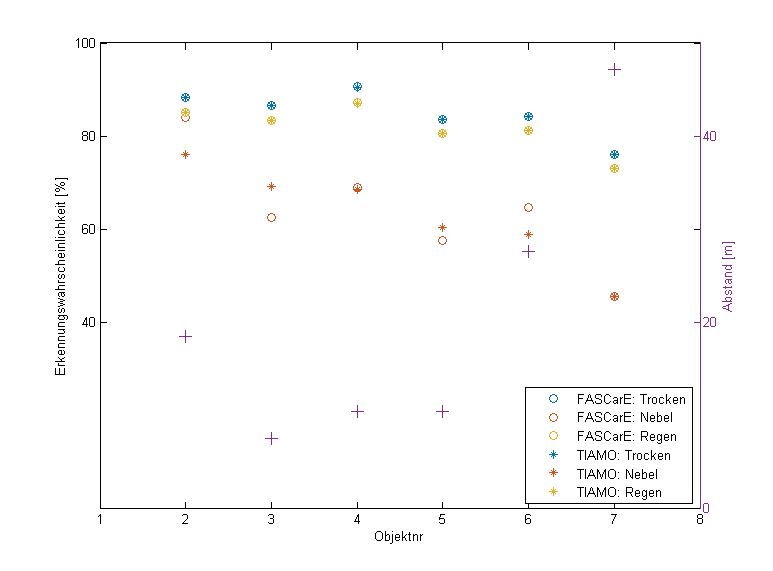
\includegraphics[width=\textwidth,trim={1cm 0.7cm 1cm 1cm},clip]{pics/VglTag_Abstand.PNG}
\caption[Erkennungswahrscheinlichkeiten von \acs{FASCarE} und \acs{TIAMO} bei Tag]{Vergleich der Erkennungswahrscheinlichkeiten vom \acs{FASCarE} und \acs{TIAMO} bei Tag zu unterschiedlichen Witterungen\label{fig:VglWahr}}
\end{figure}
\newpage
\subsection{Forschungskreuzung}
\label{sec:FoKr}
Ein weiterer Anwendungsfall ist die Analyse von Sensorkonfigurationen der Infrastruktur. Daf�r wurden die Daten der Forschungskreuzung des \acs{DLR} in Braunschweig genutzt. Die Sensorspezifikationen der Kreuzung sind in Tabelle\,\ref{tab:FoKrKonfig} aufgef�hrt. Vier Ampelmaste sind mit Kameras jedes Typs ausgestattet und auf die Kreuzungsmitte gerichtet, siehe Abbildung\,\ref{fig:FoKrT=12}. F�r die Auswertung wurden 34 Objekte innerhalb von \unit[43.52]{s} aus Daten der Forschungskreuzung ausgew�hlt. Die Trajektorien und Aufenthaltszeiten der Objekte sind in den Abbildungen\,\ref{fig:FoKrTraj} und \ref{fig:FoKrZeit} dargestellt. Da die Objektdaten des Datensatzes erst ab dem Zeitpunkt, zu dem sich das Objekt bewegt, vorliegen, wurden die Anwesenheitszeiten verl�ngert, sodass die Objekte sich um bis zu \unit[100]{ms} fr�her an der Kreuzung befinden. Au�erdem wurden Objekte, die an �hnlichen Punkten zu �hnlichen Zeiten beginnen, entlang der Fahrspur nach hinten versetzt, damit sich bei der Simulation keine Objekte aufeinander befinden. Des Weiteren wurde das Objekt\,2 mit der Sensorkonfiguration des \acs{FASCarE} ausgestattet, siehe Abbildung\,\ref{fig:FoKrT=2.08}, und das Objekt\,21 mit der vom \acs{TIAMO}, siehe Abbildung\,\ref{fig:FoKrT=20}. 

\begin{tabularx}{0.95\textwidth}{lp{1.7cm}cccc}%
\caption{Sensorkonfiguration f�r den Innenbereich der Forschungskreuzung}
\label{tab:FoKrKonfig}\\\toprule
\textbf{Anz}&\textbf{Typ}	&$\boldsymbol{\phi_H$/$\phi_V}$ \textbf{[�]}	& $\boldsymbol{R_{min}$/$R_{max}}$ \textbf{[m]}&\textbf{Tol [$\pm$m]	}& $\boldsymbol{T_{Mess}}$ \textbf{[ms]}	\\ \midrule
4&Kamera (sichtbar)&	97/74	&1/77.5	&0.25&	50	\\
4&Kamera (NIR)& 42.6/34.7&	1/77.5	&0.25&	50	\\\bottomrule
\end{tabularx} 

\begin{figure}[hbtp]%
\centering
\subfigure[][T = \unit{2.08}{s} \label{fig:FoKrT=2.08}]{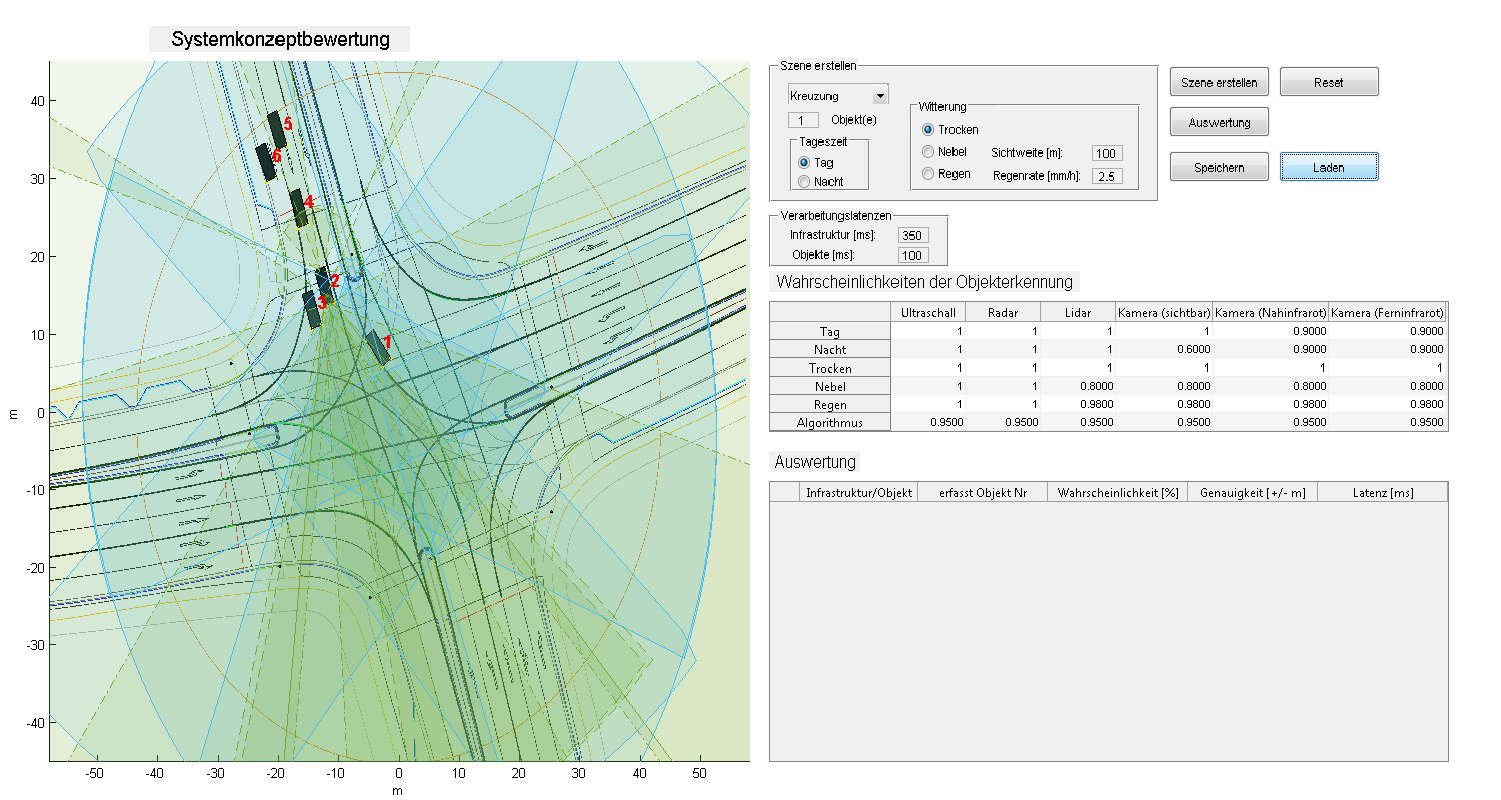
\includegraphics[width=0.33\columnwidth,trim={0.2cm 0.1cm 19.9cm 2.0cm},clip]{pics/FoKr_T=2-08.PNG}}%
\subfigure[][T = \unit{12}{s} \label{fig:FoKrT=12}]{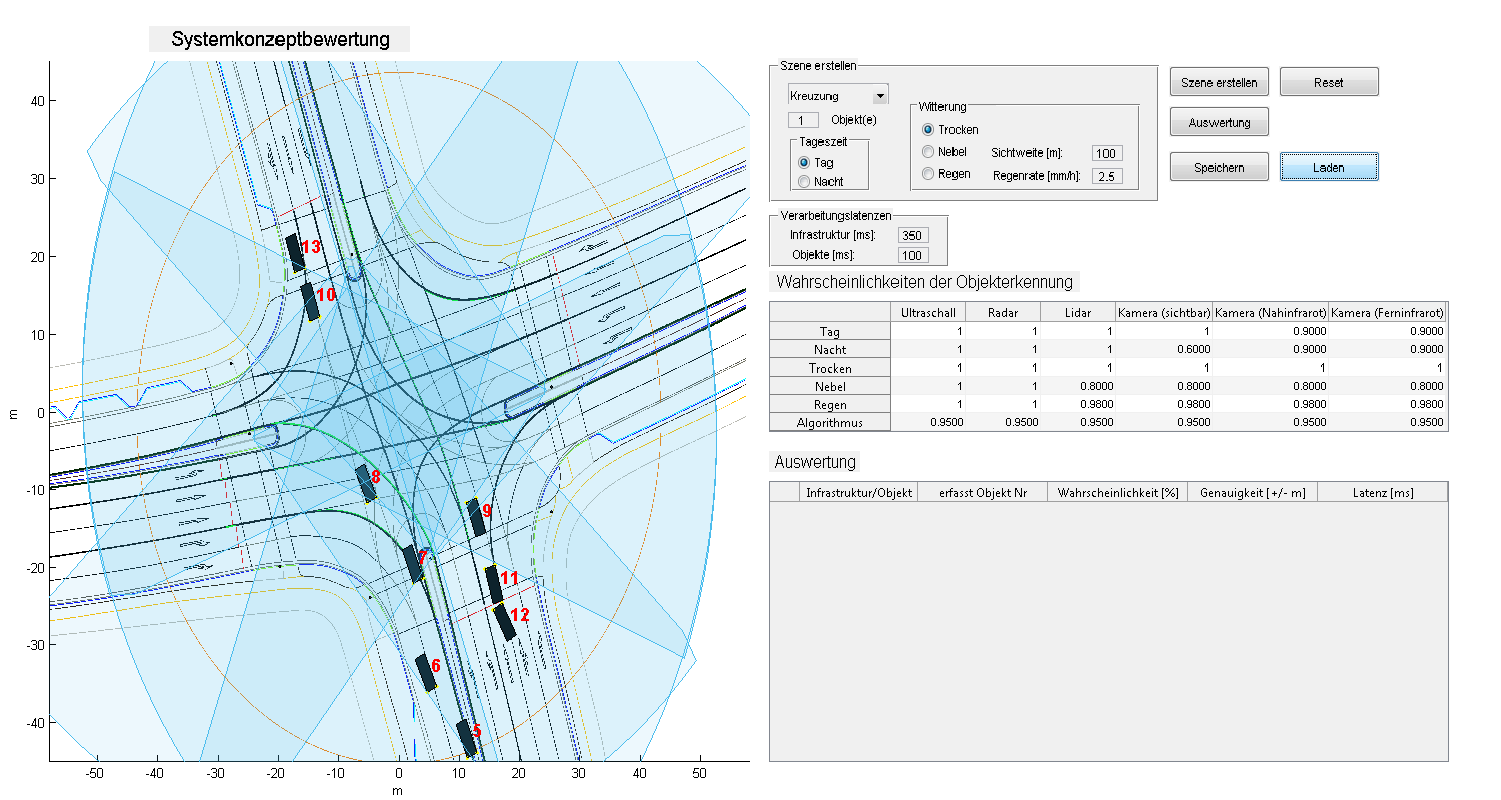
\includegraphics[width=0.33\columnwidth,trim={0.2cm 0.1cm 19.9cm 2.0cm},clip]{pics/FoKr_T=12.PNG}}
\subfigure[][T = \unit{20}{s} \label{fig:FoKrT=20}]{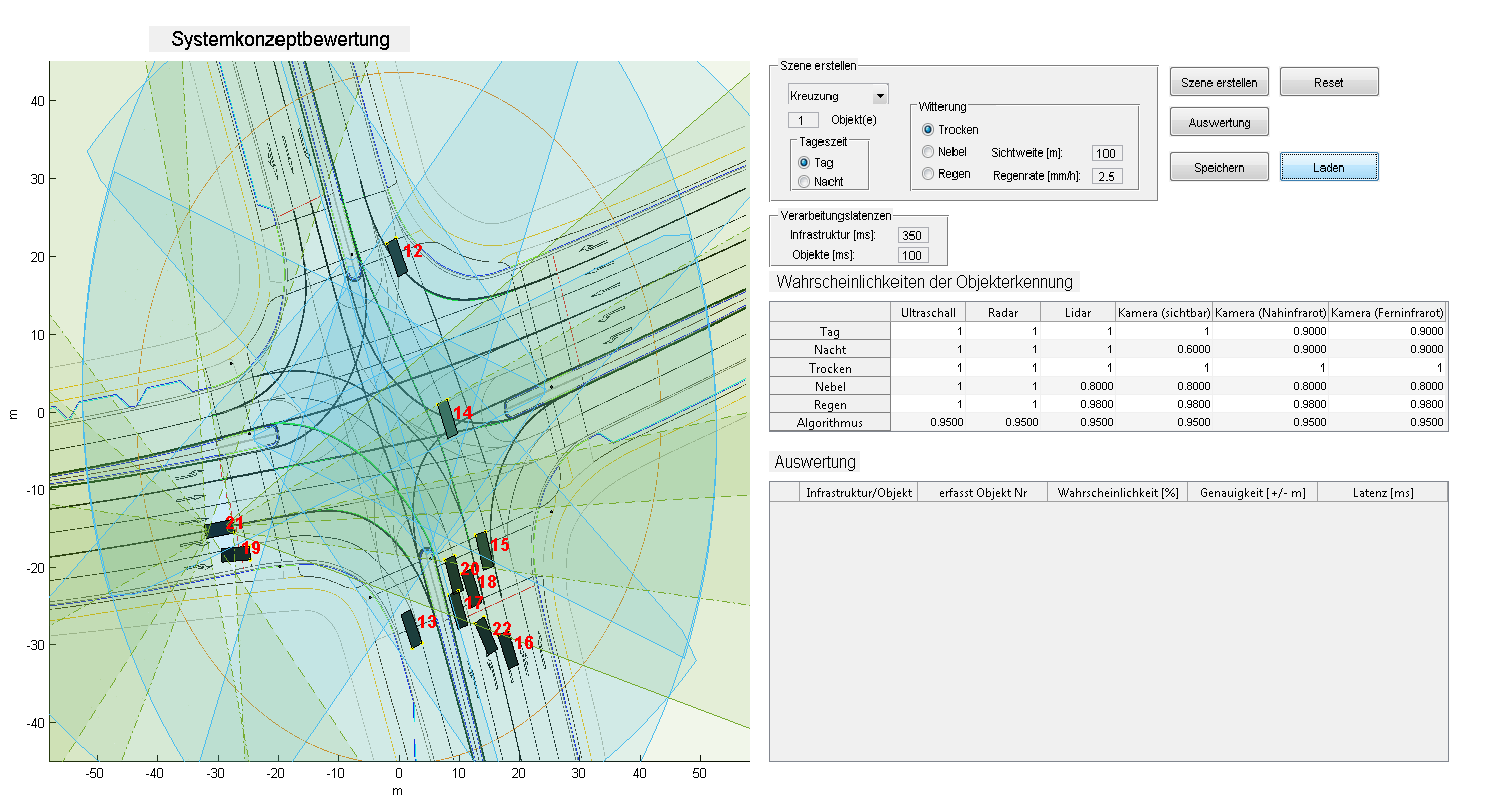
\includegraphics[width=0.33\columnwidth,trim={0.2cm 0.1cm 19.9cm 2.0cm},clip]{pics/FoKr_T=20.PNG}}
\caption[Drei Szenen auf der Forschungskreuzung]{Drei Szenen auf der Forschungskreuzung. Blau: Sichfelder der Infrastruktursensoren. Gr�n: Sichtfelder der Objektsensoren}%
\label{fig:FoKrT}%
\end{figure}

\begin{figure}[hbtp]%
\centering
\subfigure[][Trajektorien \label{fig:FoKrTraj}]{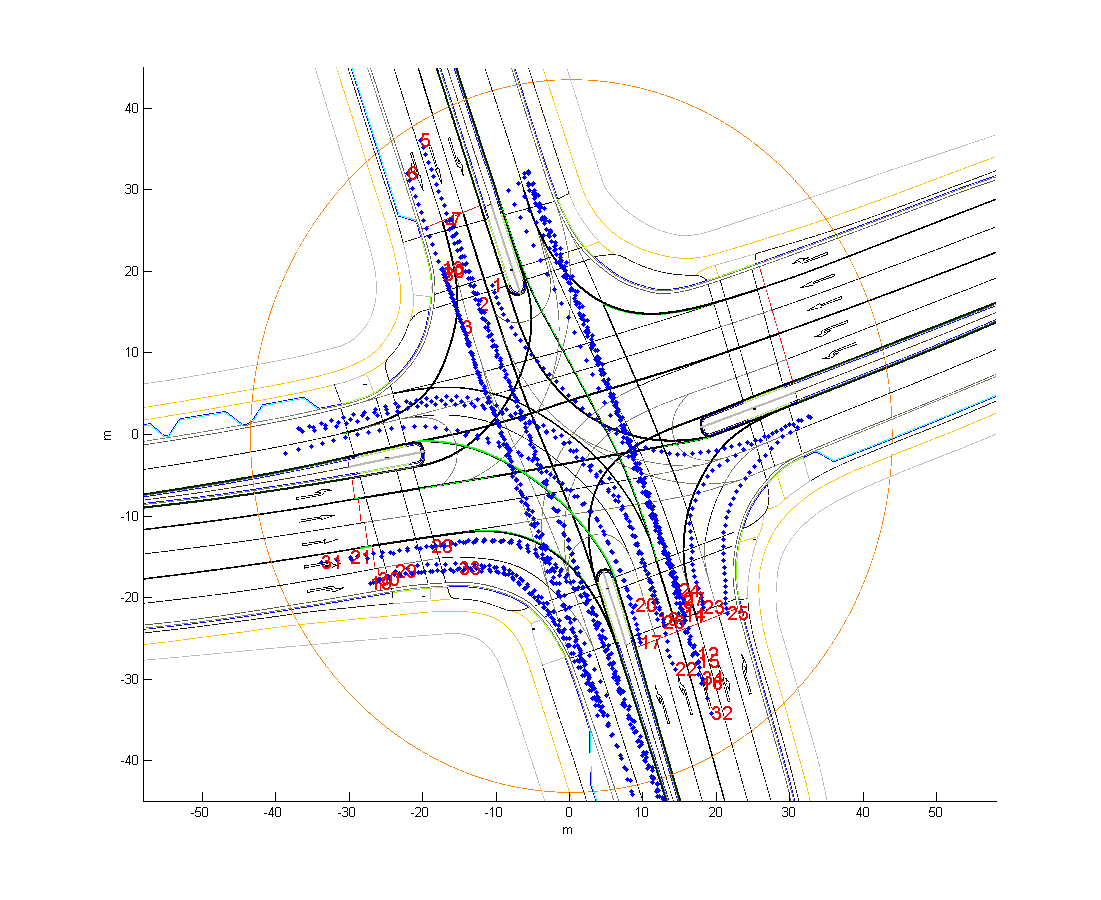
\includegraphics[width=0.8\columnwidth,trim={2cm 1.2cm 2cm 1.8cm},clip]{pics/FoKr_34Obj.PNG}}\\%
\subfigure[][Aufenthaltszeiten \label{fig:FoKrZeit}]{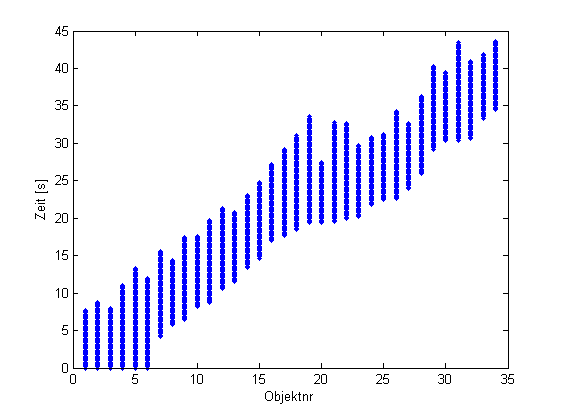
\includegraphics[width=0.7\columnwidth,trim={0.7cm 0.3cm 1.25cm 0.6cm},clip]{pics/FoKr_34Obj_Zeit.PNG}}
\caption[Objekttrajektorien und -aufenthaltszeiten auf der Forschungskreuzung]{Trajektorien und Aufenthaltszeiten von 34 Objekten auf der Forschungskreuzung}%
\label{fig:FoKr34Obj}%
\end{figure}

Abbildung\,\ref{fig:FoKr_Wahr} zeigt die Verl�ufe der Erkennungswahrscheinlichkeiten von f�nf Objekten innerhalb von \unit[35]{s} bei Tag und Nacht. Zu erkennen ist, dass zum Einen die Erkennungswahrscheinlichkeiten bei Nacht geringer sind und sich zum Anderen die Verl�ufe unterscheiden. Dies ist darauf zur�ckzuf�hren, dass sich am Tage die zwei Kameratypen gegenseitig erg�nzen und bei Nacht die Objekte haupts�chlich von der Infrarotkamera erfasst werden. Eine Auswertung am Tage mit Nebel ist in Abbildung\,\ref{fig:FoKr_WahrNebel} im Anhang zu finden. Der Nebel f�hrt ausschlie�lich zu einer Verringerung der Erkennungswahrscheinlichkeit von etwa \unit[20]{\%}. Die Spr�nge in den Verl�ufen sind auf Sichtfeldwelchsel der Objekte, w�hrend sie die Kreuzung �berqueren, zur�ckzuf�hren. 

\begin{figure}[hbtp]%
\centering
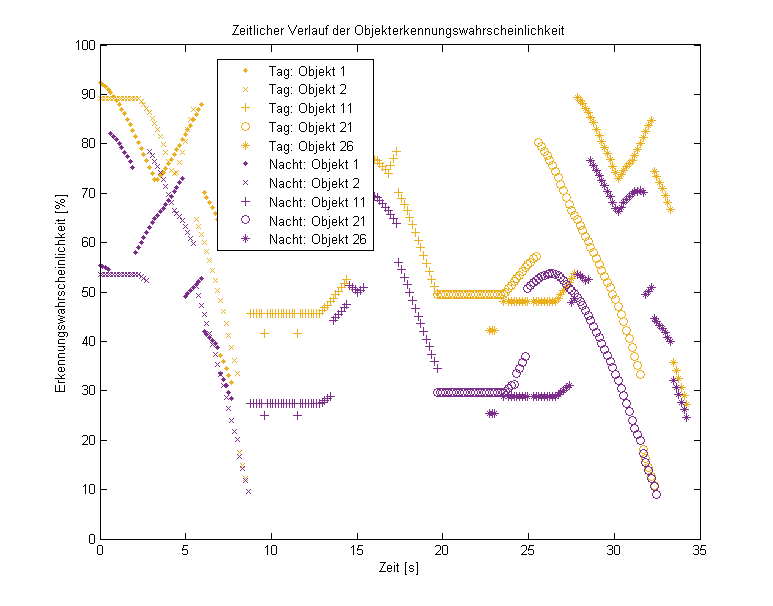
\includegraphics[width=\textwidth,trim={1cm 0.8cm 1.7cm 1.05cm},clip]{pics/FoKr_TagNacht.PNG}
\caption[Erkennungswahrscheinlichkeiten der Forschungskreuzung]{Erkennungswahrscheinlichkeiten der Forschungskreuzung von f�nf Objekten bei Tag und bei Nacht\label{fig:FoKr_Wahr}}
\end{figure} 

Eine weitere Einsatzm�glichkeit ist der Vergleich der Erkennungswahrscheinlichkeiten eines mit Sensorik ausgestatteten Fahrzeugs und der Infrastruktursensoren. Abbildung\,\ref{fig:VglFoKrFASCarE} zeigt hierf�r die Verl�ufe der Erkennungswahrscheinlichkeiten des \acs{FASCarE} und der Forschungskreuzung. F�r die Fahrsituation, bei der das \acs{FASCarE} geradeaus von Nord nach S�d �ber die Kreuzung f�hrt, fallen die Erkennungswahrscheinlichkeiten beim \acs{FASCarE} h�her aus als die der Infrastruktur. Bei der Erfassung von Objekt\,3 hingegen bricht die Wahrscheinlichkeit beim \acs{FASCarE} f�r etwa \unit[2]{s} ein. Dies k�nnte per \acs{C2X}-Kommunikation in diesem Zeitraum von der Forschungskreuzung aufgefangen werden. Die Erkennungswahrscheinlichkeiten f�r die Objekte\,4 und 6 fallen bei der Forschungskreuzung deutlich geringer aus als beim \ac{FASCarE}, da sie sich im nahen Umfeld des \acs{FASCarE} befinden, was aufgrund des geringeren Abstandes zu einer h�heren Erkennungswahrscheinlichkeit f�hrt.

\begin{figure}[hbtp]%
\centering
\subfigure[][\acs{FASCarE}\label{fig:VglFoKrFASCarE}]{\includegraphics[width=\textwidth,trim={0.7cm 0.3cm 0cm 0.6cm},clip]{pics/Vgl_FoKrFASCarE.PNG}}\\
\subfigure[][\acs{TIAMO}\label{fig:VglFoKrTIAMO}]{\includegraphics[width=\textwidth,trim={0.7cm 0.3cm 0.1cm 0.7cm},clip]{pics/Vgl_FoKrTIAMO.PNG}}%
\caption[Vergleich der Erkennungswahrscheinlichkeiten der Forschungskreuzung]{Vergleich der Erkennungswahrscheinlichkeiten der Forschungskreuzung mit denen des \acs{FASCarE} und des \acs{TIAMO}\label{fig:Vgl}}
\end{figure}

Das gleiche trifft auch auf die Verl�ufe des \acs{TIAMO} und der Forschungskreuzung in Abbildung\,\ref{fig:VglFoKrTIAMO} zu. Die Fahrsituation hier ist, dass das \acs{TIAMO} von Westen aus kommend rechts abbiegt und nach S�den f�hrt. Hier k�nnten die erfassten Daten von Objekt\,17 von der Forschungskreuzung in den ersten \unit[2]{s} per \acs{C2X}-Kommunikation an das \acs{TIAMO} weitergegeben werden.

\subsection{Evaluation}
\label{sec:Evaluation}
Die Analyse der vier Szenen zeigt, dass folgende Einfl�sse auf die Objekterkennung im Simulations-Tool ber�cksichtigt werden: Objektabstand, Tageszeit, Witterung, Objekterkennungsalgorithmus. Eine erste Auslegung von Sensorkonfigurationen f�r Fahrzeuge und f�r Infrastrukturelemente ist somit bereits m�glich. F�r die Systemauslegung gibt das Tool aus, welche Objekte erfasst werden und mit welcher Wahrscheinlichkeit, welcher Genauigkeit und welcher Latenz dies geschieht. Bei der Objekterfassung werden jedoch bislang keine sichtverdeckende Elemente wie H�user und B�ume ber�cksichtigt. Des Weiteren wurde die Sensordatenfusion nur mit einem simplen Ansatz umgesetzt. Daf�r wurde zum Einen bei der Erkennungswahrscheinlichkeit der gr��te Wert einer Sensorkonfiguration genutzt und zum Anderen bei der Genauigkeit und der Latenz nur die Daten des Sensors mit der geringsten Latenz. Dadurch, dass mit dem Tool nur explizite Zeitpunkte untersucht werden k�nnen, wird au�erdem nicht ber�cksichtigt, dass sich die Erkennungswahrscheinlichkeit eines Objektes durch ein Objekttracking mit der Zeit erh�ht. 


\section{Zusammenfassung und Ausblick}
\label{sec:Zusammenfassung}
%\section{Beispielkapitel}
Dies ist ein Beispieltext.

\subsection{Unterkapitel 1}\label{Unterkapitel1Link}
Beispiel f�r eine Fu�note\footnote{Fu�noten sind gut.}.

\begin{figure}[htbp]
	\centering
		\includegraphics[width=1.0\textwidth]{pics/accBosch.pdf}
	\caption{Folgefahrt Beispielbild}
	\label{fig:accBosch}
\end{figure}

Wie in \ref{Unterkapitel1Link} gezeigt, ist es m�glich, Kapitel zu verlinken. Abk�rzungen wie das \ac{IfF} werden so dargestellt. Quellen �brigens so \citep{ams09}.

Abbildung ~\ref{fig:accBosch} soll ein Beispielhaftes Bild zeigen.


\subsubsection{Unterunterkapitel1} 

\textbf{\sffamily{M�glichkeit zur weiteren Unterteilung -- Teilkapitel}} Mehr als drei Unterteilungsebenen sollen vermieden werden!
\par
\begingroup
\leftskip=0.8cm
\noindent \textbf{\sffamily{Einger�cktes Teilkapitel}} Derartige Dinge wie einger�ckte Teilkapitel gibt es auch. Falls Du sie brauchen solltest.
\par
\endgroup

\begin{table}[ht]
\caption{Tabular Umgebung: Simpel formatierte Tabelle}
 \small
	\centering
		\begin{tabular}{ll}
		  \toprule
			\multicolumn{2}{c}{Zwei miteinander verbundene Zellen}\\
		  \midrule
			Punkt 1 & Adaptive Cruise Control\\
			Punkt 2 & Lane Keeping Assist\\			
			\toprule
			\multicolumn{2}{c}{Schon wieder zwei miteinander verbundene Zellen}\\
		  \midrule
			Punkt 3 & Elektronisches Stabilit�tsprogramm\\
			\toprule
		\end{tabular}
	\label{tab:Tabular1}
\end{table}

\begin{table}[h]
 \caption{Tabular Umgebung: Etwas komplexere Tabelle}
	\centering
		  \begin{tabular}{|c|c|c|c|c|c|c|c|c|c|}
				\cline{2-10}
				\multicolumn{1}{c|}{} & \rotatebox{90}{Fahrzeug-CAN} & \rotatebox{90}{GPS-System} & \rotatebox{90}{ESP-Cluster} & \rotatebox{90}{Correvit} & \rotatebox{90}{Lichtschranke} & \rotatebox{90}{Radar} & \rotatebox{90}{Lidar} & \rotatebox{90}{Kreiselplattform} & \rotatebox{90}{Webcam, Leuchtdiode} \\
				\hline
				\multicolumn{10}{|c|}{}  \\
				\multicolumn{1}{|c}{\bfseries{Subjekt}} & \multicolumn{9}{c|}{}  \\
				\hline
				\hline	
				\multicolumn{1}{|c|}{Setzgeschwindigkeit}  &  &  &  &  &  &&  &  & x\\		
				\hline	
				\multicolumn{10}{|c|}{}  \\
				\multicolumn{1}{|c}{\bfseries{relative Gr��en}} & \multicolumn{9}{c|}{}  \\
				\hline
				\multicolumn{1}{|c|}{Triggersignal}  &  & x &   &  & x &   &  & & x \\		
				\hline	
				\multicolumn{10}{|c|}{}  \\
				\multicolumn{1}{|c}{\bfseries{Objekt}} & \multicolumn{9}{c|}{}  \\
				\hline
				\multicolumn{1}{|c|}{L�ngsgeschwindigkeit} & x  & x &  & x &   &  &&   &    \\	
				\hline
				\end{tabular}
	    \label{tab:sensorik}
\end{table}

Nachfolgend das Beispiel f�r eine Aufz�hlung mit Itemize.
\begin{itemize}
  \item Reaktionszeit $\mathrm{\Delta t_{react}}$
  \item Im oberen Punkt sieht man auch sch�n die Einbindung von Formeln in den Text.
\end{itemize}

$v_{Obj.}$ = 120\,km/h \\
Einheiten sollten nicht kursiv dargestellt werden und werden vom Zahlenwert durch ein schmales Leerzeichen (Backslash und Komma) getrennt.

Es gibt eine Vielzahl von Gleichungsumgebungen. Equation ist eine davon. Die Gleichung ergibt nat�rlich keinen tieferen Sinn:
\begin{equation}
	x_{obj} = \frac{s^{2} \cdot a \cdot \sqrt{b}}{234 \cdot h_{ego}}
\end{equation}

\bibliographystyle{alphadin}
\bibliography{Literatur}
\setcounter{secnumdepth}{-1}
\section{Anhang}
\setcounter{secnumdepth}{3}

%\subsection*{Hier sind zus�tzliche Infos einzubringen}
%
%Das Beispiel f�r eine Tabbing Umgebung zeigt, dass es m�glich ist, mehrere Zeilen mit dem gleichen Einzug darzustellen:
%\begin{tabbing}
%\hspace{1.3cm}\=\hspace{2.7cm}\=\hspace{3cm}\=\kill
%$v_{Start}$ \>= 120\,km/h \>= 33,3\,m/s\\
%$v_{End}$ \>= 80\,km/h \>= 22,2\,m/s\\
%\newline
%$v_{Diff}$ \>= 40\,km/h \>= 11,1\,m/s\\
%\end{tabbing}
\subsection*{Vergleich der Sensorkonfigurationen vom \acs{FASCarE} und \acs{TIAMO}}
\begin{figure}[hbtp]%
\centering
\includegraphics[width=\textwidth,trim={1cm 0.7cm 1cm 1cm},clip]{pics/VglNacht_Abstand.PNG}%
\caption[Erkennungswahrscheinlichkeiten von \acs{FASCarE} und \acs{TIAMO} bei Nacht]{Vergleich der Erkennungswahrscheinlichkeiten vom \ac{FASCarE} und \ac{TIAMO} bei Nacht zu unterschiedlichen Witterungen\label{fig:VglWahrNacht}}
\end{figure}
\newpage
\subsection*{Forschungskreuzung}
\begin{figure}[hbtp]%
\centering
\includegraphics[width=0.9\textwidth,trim={0.7cm 0.2cm 1cm 0.7cm},clip]{pics/FoKr_WahrNebel_Obj=1,2,21,26,11,16.PNG}
\caption[Erkennungswahrscheinlichkeiten der Forschungskreuzung bei Nebel]{Erkennungswahrscheinlichkeiten der Forschungskreuzung von sechs Objekten bei Nebel\label{fig:FoKr_WahrNebel}}
\end{figure} 


\begin{landscape}
\subsection*{Sensorspezifikationen}
	
\begin{tabularx}{1.4\textwidth}{Xcccccc}%1.45 Xp{1.2cm}p{1cm}p{1.6cm}p{1.6cm}p{1cm}Xp{2cm}X
		\caption{Spezifikationen einer Auswahl von Sensoren}
	\label{tab:SensorSpec}\\\toprule
\textbf{Sensor}&$\boldsymbol{\phi_H}$/$\boldsymbol{\phi_V}$ \textbf{[�]}&$\boldsymbol{R_{min}}$/$\boldsymbol{R_{max}}$ \textbf{[m]}&$\boldsymbol{\Delta\phi_H}$\textbf{[�]}&\textbf{Tol [$\pm$m]}&$\boldsymbol{T_{Mess}}$ \textbf{[ms]}&\textbf{Hersteller}\\\midrule\endfirsthead
\caption*{Spezifikationen einer Auswahl von Sensoren}
	\label{tab:SensorSpec}\\\toprule
\textbf{Sensor}&$\boldsymbol{\phi_H}$/$\boldsymbol{\phi_V}$ \textbf{[�]}&$\boldsymbol{R_{min}}$/$\boldsymbol{R_{max}}$ \textbf{[m]}&$\boldsymbol{\Delta\phi_H}$\textbf{[�]}&\textbf{Tol [$\pm$m]}&$\boldsymbol{T_{Mess}}$ \textbf{[ms]}&\textbf{Hersteller}\\\midrule\endhead
\midrule\endfoot 
\bottomrule\endlastfoot
		
Ultraschall&120/60&0.15/1.5&10&-&1&-\\
Ultraschall&140/70&0.15/5.5&10&-&1&Bosch\\
Ultraschall&50/50&0.15/5&10&-&1&-\\\midrule
Radar&17/23.1&0.8/50&1&0.36&66&-\\
Radar&18/23.1&0.2/120&3.3&0.36&60&Continental\\
Radar&90/23.1&0.2/40&6.6&0.36&60&Continental\\
Radar&12/23.1&0.36/0.72&7&0.12&60&Bosch\\
Radar&10/23.1&0.36/0.72&7&0.12&60&Bosch\\
Radar&150/23.1&0.36/0.72&7&0.12&60&Bosch\\
Radar&20/4.5&1/60&5.3&0.5&50&Delphi\\
Radar&90/4.5&1/174&5.3&0.5&50&Delphi\\
Radar&150/10&0.5/80&5.3&0.36&50&Delphi\\
Radar&36/8&1/160&5.3&0.25&50&SmartMicro\\
Radar&70/10&1/90&5.3&0.25&50&SmartMicro\\
Radar&100/10&1/45&5.3&0.25&50&SmartMicro\\
Radar&36/12&1.5/450&5.3&0.25&79&SmartMicro\\
Radar&100/36&1.5/340&5.3&0.25&53&SmartMicro\\
Radar&100/16&1.5/330&5.3&0.25&79&SmartMicro\\
Radar&80/24&1/120&5.3&0.25&75&SmartMicro\\
Radar&80/12&1/120&5.3&0.25&75&SmartMicro\\
Radar&15/130&0.4/55&5.3&0.55&50&SmartMicro\\
Radar&66/23.1&0.82/70&5.3&0.36&60&SmartMicro\\
Radar&140/23.1&0.82/8&5.3&0.36&60&SmartMicro\\
Radar&16/23.1&0.82/120&5.3&0.36&60&SmartMicro\\
Radar&36/23.1&0.8/99&5.3&0.36&60&Jenoptik\\
Radar&165/23.1&0.75/70&5.3&1.50&50&Hella\\\midrule
Lidar&180/20.2&0.6/100&0.31&0.05&99&-\\
Lidar&27/11&1/13.5&0.31&0.1&80&Continental\\
Lidar&110/3.2&0.3/200&0.125&0.05&80&Ibeo\\
Lidar&110/3.2&0.3/120&0.125&0.05&160&Ibeo\\
Lidar&110/6.4&0.3/200&0.125&0.05&40&Ibeo\\
Lidar&145/3.2&0.3/327&0.25&0.05&25&Ibeo\\
Lidar&270/20.2&0.1/80&0.25&0.03&25&Hokuyo\\
Lidar&270/20.2&0.06/5&0.5&0.04&25&Hokuyo\\
Lidar&270/20.2&0.02/20&0.25&0.04&50&Hokuyo\\
Lidar&190/20.2&0.1/80&0.25&0.05&20&Hokuyo\\
Lidar&95/20.2&0.6/100&0.563&0.05&10&Leddartech\\
Lidar&20/3&0.6/60&2.5&0.05&333&Leddartech\\
Lidar&360/70&0.6/160&0.31&0.05&333&Ocular\\
Lidar&360/70&0.6/270&0.31&0.05&200&Ocular\\
Lidar&360/30&1/100&0.2&0.05&200&Velodyne\\
Lidar&360/40&1/100&0.2&0.05&200&Velodyne\\
Lidar&360/26.9&1/120&0.17&0.05&50&Velodyne\\
Lidar&90/20.2&1.6/250&0.023&0.05&50&Triple-IN\\
Lidar&90/20.2&0.6/170&0.023&0.05&200&Triple-IN\\
Lidar&90/20.2&2.1/300&0.023&0.05&99&Triple-IN\\
Lidar&270/20.2&0.8/160&0.045&0.05&40&Triple-IN\\
Lidar&270/20.2&2/200&0.045&0.05&66&Triple-IN\\
Lidar&360/45&0.6/1000&0.31&0.05&80&Neptec\\
Lidar&270/20.2&0.5/50&0.25&0.05&80&SICK\\
Lidar&270/20.2&0.05/8&1&0.05&80&SICK\\
Lidar&275/7.5&0.2/64&0.25&0.05&100&SICK\\
Lidar&110/3.2&0.5/300&0.125&0.05&40&SICK\\
Lidar&110/3.2&0.5/300&0.125&0.05&80&SICK\\
Lidar&120/15&0.5/75&0.13&0.05&33&SICK\\
Lidar&190/20.2&0.5/40&0.167&0.025&99&SICK\\
Lidar&190/20.2&0/80&0.25&0.025&13&SICK\\
Lidar&110/3.2&0.6/90&0.25&0.1&99&Ibeo LUX\\\midrule
Kamera (sichtbar)&50/28&1/120&0&-&33&Bosch\\
Kamera(sichtbar)&97/74&1/77.5&1&-&50&AVT\\
Kamera(\acs{FIR})&9/6.7&1/285&1&-&33&Riva\\
Kamera(\acs{FIR})&24/18&1/100&1&-&33&Riva\\
Kamera(\acs{FIR})&41.8/31.4&1/60&1&-&33&Riva\\
Kamera(\acs{FIR})&17.6/13.2&1/285&1&-&0.1&Riva\\
Kamera(\acs{FIR})&37.5/28&1/140&1&-&31&Riva\\
Kamera(\acs{FIR})&49.8/37&1/100&1&-&33&Riva\\
Kamera(\acs{NIR})&100/54&1/35&1&-&50&Riva\\
Kamera(\acs{NIR})&42.6/34.7&1/77.5&1&-&50&AVT\\
Kamera(\acs{NIR})&97/74&1/77.5&1&-&50&AVT\\\bottomrule
\end{tabularx}

\end{landscape}



\end{document}
